\chapter{The HiSPARC Experiment}
\label{ch:hisparc-experiment}

Propagating charged particles lose energy in matter. In scintillators, the
energy loss can be observed in the form of light. \hisparc employs scintillator
detectors to detect EAS. In this chapter, the experimental setup is discussed
in detail. In \secref{sec:design-criteria} the design criteria are presented.
\secref{sec:hisparc-overview} discusses detector physics and the geometry of the
\hisparc station. \secref{sec:data-acquisition} describes the signal
characteristic, the trigger, and the data acquisition system.
\secref{sec:features-pulseheight-spectrum} discusses some features of
the pulseheight spectrum. \secref{sec:features-time-spectrum} discusses
the timing between stations. Finally, in \secref{sec:hisparc-locations} an
overview of the \hisparc locations of stations in the Netherlands is given.

In \hisparc the distances between clusters of \hisparc stations ranges from tens
of kilometers to hundreds of kilometers.  \hisparc is therefore ideally suited
to study long-range correlations between cosmic ray showers.


\section{Design Criteria}
\label{sec:design-criteria}

The purpose of the \hisparc experiment is to detect air showers and reconstruct
shower direction and energy.  However, due to the collaboration with high
schools, resources are limited.
The majority of detectors is financed by high schools, while students are
responsible for assembly and subsequent installation on the roof of their high
school.  Therefore, detectors should be cheap, robust and easily
maintainable (e.g.
scintillators).
The geometry of the detector network is constrained by the geographical location
of each high school.


\subsection{Extensive Air Showers}
\label{sec:design-criteria-EAS}

High energy cosmic ray particles generate cascades in the atmosphere. The number
of particles in an EAS depends on the energy and nature of the primary particle,
as well as the first series of particle interactions.
The particle density in an EAS falls steeply with increasing distance to the
center of the shower (core distance). The \emph{lateral distribution} for a few
particle types in an \SI{1}{\peta\electronvolt} proton EAS is depicted in
\figref{fig:lateral_distribution}.

For charged particles, the efficiency of scintillator detectors is close to
\SI{100}{\percent}.
The probability that exactly $k$ charged particles are detected is given by the
\emph{Poisson distribution}
\begin{equation}
P_k(\lambda) = \frac{\lambda^k e^{-\lambda}}{k!},
\end{equation}
with $\lambda$ the \emph{expected} number of detected particles. The probability
of detecting \emph{zero} particles then becomes
\begin{equation}
P_0(\lambda) = e^{-\lambda}.
\end{equation}
The probability of detecting at least one particle
is then given by
\begin{equation}
P_p(\lambda) = 1 - P_0(\lambda).
\end{equation}
For a scintillator surface area of \SI{0.5}{\square\meter}, $\lambda = \num{0.5}
\rho$, with $\rho$ the particle density. The
particle density at which a single scintillator has a \SI{50}{\percent}
detection probability is then calculated to be
\SI{1.39}{\per\square\meter}.

A single scintillator can not distinguish between charged particles that are
part of a shower, or stray particles not correlated to any shower.  Low-energy
primary particles are much more abundant than high-energy particles.  This
results in a large number of showers of which only a few particles reach the
ground. These spurious charged particles, mainly muons, form the background (see
\secref{sec:fluxes}).

However, observation of coincident signals in two scintillators that are a few
meters apart, decreases the probability that the particles are uncorrelated.
Coincidences are predominantly due to EAS.  For two detectors, the probability
of detecting a particle in both (given a particle density $\rho$) is
$P_p(\rho)^2$.  The particle density at which the combination of two detectors
has a \SI{50}{\percent} probability of recording at least one particle in each
detector becomes \SI{2.46}{\per\square\meter}.

\figref{fig:ldf-threshold} shows the lateral distribution function (LDF) summed
over electrons and positrons in proton-induced EAS. Primary energies ranging
from \SI{e14}{\electronvolt} to \SI{e18}{\electronvolt} are depicted. For EAS
with primary energies of \SI{e14}{\electronvolt}, the particle densities are too
low to reach a detection probability of \SI{50}{\percent} for any core distance.
A two-detector setup will only measure EAS of \SI{e15}{\electronvolt} up to
\SI{20}{\meter} with probabilities higher than \SI{50}{\percent}. EAS of
\SI{e17}{\electronvolt}, on the other hand, can be detected at distances up to
\SI{200}{\meter}.
\begin{figure}
\centering
{\pgfkeys{/artist/width/.initial=.5\linewidth}
\pgfkeys{/artist/height/.initial=.7\linewidth}
% \usepackage{tikz}
% \usetikzlibrary{arrows,pgfplots.groupplots}
% \usepackage{pgfplots}
% \pgfplotsset{compat=1.3}
% \usepackage[detect-family]{siunitx}
% \usepackage[eulergreek]{sansmath}
% \sisetup{text-sf=\sansmath}
% \usepackage{relsize}
%
\pgfkeysifdefined{/artist/width}
    {\pgfkeysgetvalue{/artist/width}{\defaultwidth}}
    {\def\defaultwidth{ .45\linewidth }}
%
\pgfkeysifdefined{/artist/height}
    {\pgfkeysgetvalue{/artist/height}{\defaultheight}}
    {\def\defaultheight{ .6\linewidth }}
%
\begin{sansmath}
\begin{tikzpicture}[font=\sffamily]
\node[inner sep=0pt] (plot) {
    \begin{tikzpicture}[
            inner sep=.3333em,
            font=\sffamily,
            every pin/.style={inner sep=2pt, font={\sffamily\smaller}},
            every label/.style={inner sep=2pt, font={\sffamily\smaller}},
            every pin edge/.style={<-, >=stealth', shorten <=2pt},
            pin distance=2.5ex,
        ]
        \begin{groupplot}[
                xmode=log,
                ymode=log,
                width=\defaultwidth,
                height=\defaultheight,
                %
                xmin={ 6 },
                xmax={ 2500 },
                ymin={ 1e-06 },
                ymax={ 100000.0 },
                %
                group style={rows=1,columns=2,
                             horizontal sep=4pt, vertical sep=4pt},
                %
                tick align=outside,
                max space between ticks=40,
                every tick/.style={},
                %
                xtick=\empty, ytick=\empty,
                scaled ticks=false,
            ]
            
                
                \nextgroupplot[
                    % Default: empty ticks all round the border of the
                    % multiplot
                        xtick={  },
                        xtick pos=both,
                        xticklabel=\empty,
                        ytick={ 1e-6, 1e-4, 1e-2, 1e0, 1e2, 1e4 },
                        ytick pos=left,
                        yticklabel=\empty,
                        xticklabel={},
                        yticklabel={},
                    title={ Electrons },
                    xlabel={  },
                    ylabel={  },
                ]

                

                

                
                    \addplot[no markers,solid] coordinates {
                        (11.4163099875, 0.224534600105)
                        (13.0332133731, 0.187684857541)
                        (14.8791204001, 0.161882801065)
                        (16.986465083, 0.141751558925)
                        (19.392275098, 0.123834296093)
                        (22.1388223882, 0.106361673737)
                        (25.2743659142, 0.0843386623902)
                        (28.8539996015, 0.0649389764522)
                        (32.9406203831, 0.0537269044274)
                        (37.6060333475, 0.0429501174474)
                        (42.9322134096, 0.0323247283827)
                        (49.0127456735, 0.0248005049206)
                        (55.9544697949, 0.0191279833484)
                        (63.8793572367, 0.0149387557802)
                        (72.9266544018, 0.0118985758221)
                        (83.2553293004, 0.00887917479622)
                        (95.0468647408, 0.00610912398865)
                        (108.508447122, 0.00452143339183)
                        (123.876606861, 0.00357117611815)
                        (141.421374413, 0.00267999952099)
                        (161.451024917, 0.00194811618122)
                        (184.317494825, 0.00143416277594)
                        (210.422565705, 0.00109185990564)
                        (240.224923846, 0.000811815006357)
                        (274.248219736, 0.00058528167999)
                        (313.090269003, 0.000433105019408)
                        (357.433556502, 0.00032059672116)
                        (408.057228097, 0.000237577474699)
                        (465.850780861, 0.000171008239205)
                        (531.829692224, 0.000118912270211)
                        (607.1532627, 8.09549351896e-05)
                        (693.144985692, 5.43884708725e-05)
                        (791.315802296, 3.98129056326e-05)
                        (903.390649705, 2.91339764409e-05)
                        (1031.33876969, 2.06044340508e-05)
                        (1177.40830969, 1.54518004909e-05)
                        (1344.16582453, 1.03597635644e-05)
                        (1534.54137275, 6.07704505665e-06)
                    };
                
                    \addplot[no markers,solid] coordinates {
                        (11.4163099875, 5.33017898745)
                        (13.0332133731, 4.51349863314)
                        (14.8791204001, 3.71387261416)
                        (16.986465083, 3.06819101573)
                        (19.392275098, 2.50997583228)
                        (22.1388223882, 2.1136174093)
                        (25.2743659142, 1.72106622027)
                        (28.8539996015, 1.32237346032)
                        (32.9406203831, 1.04015636367)
                        (37.6060333475, 0.84547414292)
                        (42.9322134096, 0.665304309238)
                        (49.0127456735, 0.493376487979)
                        (55.9544697949, 0.368921240759)
                        (63.8793572367, 0.27812246561)
                        (72.9266544018, 0.203581477472)
                        (83.2553293004, 0.15129503013)
                        (95.0468647408, 0.111963013434)
                        (108.508447122, 0.0811668120657)
                        (123.876606861, 0.0592456100393)
                        (141.421374413, 0.0418074086755)
                        (161.451024917, 0.0294718807552)
                        (184.317494825, 0.0207534254129)
                        (210.422565705, 0.0142295525531)
                        (240.224923846, 0.0106239490157)
                        (274.248219736, 0.00799587084314)
                        (313.090269003, 0.00533636443966)
                        (357.433556502, 0.00340839593889)
                        (408.057228097, 0.00231115052381)
                        (465.850780861, 0.00165794959776)
                        (531.829692224, 0.00117813831249)
                        (607.1532627, 0.000872420874187)
                        (693.144985692, 0.000622044654759)
                        (791.315802296, 0.000384724284162)
                        (903.390649705, 0.000253650508034)
                        (1031.33876969, 0.000178468709033)
                        (1177.40830969, 0.000110294907255)
                        (1344.16582453, 6.70995185105e-05)
                        (1534.54137275, 4.65632243822e-05)
                    };
                
                    \addplot[no markers,solid] coordinates {
                        (11.4163099875, 87.6694146808)
                        (13.0332133731, 74.4766600949)
                        (14.8791204001, 60.4011774591)
                        (16.986465083, 49.1678933351)
                        (19.392275098, 40.5617371532)
                        (22.1388223882, 32.6095274102)
                        (25.2743659142, 25.5133528047)
                        (28.8539996015, 20.1895630228)
                        (32.9406203831, 15.5335064851)
                        (37.6060333475, 11.4577090868)
                        (42.9322134096, 8.56613248105)
                        (49.0127456735, 6.46170294756)
                        (55.9544697949, 4.88635747648)
                        (63.8793572367, 3.64154192424)
                        (72.9266544018, 2.61359306349)
                        (83.2553293004, 1.85420969443)
                        (95.0468647408, 1.33740896893)
                        (108.508447122, 0.961375292321)
                        (123.876606861, 0.66316101448)
                        (141.421374413, 0.467689714552)
                        (161.451024917, 0.346279309116)
                        (184.317494825, 0.245271454505)
                        (210.422565705, 0.165629718922)
                        (240.224923846, 0.113353045413)
                        (274.248219736, 0.0815373945348)
                        (313.090269003, 0.0580163378717)
                        (357.433556502, 0.038822570058)
                        (408.057228097, 0.0266383184931)
                        (465.850780861, 0.0183223927609)
                        (531.829692224, 0.011766153716)
                        (607.1532627, 0.00749604975248)
                        (693.144985692, 0.00506235895821)
                        (791.315802296, 0.0033978452599)
                        (903.390649705, 0.0021094311886)
                        (1031.33876969, 0.00139292541526)
                        (1177.40830969, 0.000973378708506)
                        (1344.16582453, 0.000595210986541)
                        (1534.54137275, 0.000351617840816)
                    };
                
                    \addplot[no markers,solid] coordinates {
                        (11.4163099875, 1491.22189039)
                        (13.0332133731, 1225.67804813)
                        (14.8791204001, 1007.88844111)
                        (16.986465083, 816.619552294)
                        (19.392275098, 665.742185895)
                        (22.1388223882, 539.4135879)
                        (25.2743659142, 425.775939204)
                        (28.8539996015, 328.3725626)
                        (32.9406203831, 249.843622567)
                        (37.6060333475, 192.269678909)
                        (42.9322134096, 147.686258038)
                        (49.0127456735, 111.720156496)
                        (55.9544697949, 81.6091361556)
                        (63.8793572367, 57.473733445)
                        (72.9266544018, 40.6263602677)
                        (83.2553293004, 28.9950149861)
                        (95.0468647408, 20.7336799642)
                        (108.508447122, 15.1463168914)
                        (123.876606861, 10.7802504848)
                        (141.421374413, 7.42323234139)
                        (161.451024917, 5.39554666938)
                        (184.317494825, 3.876479531)
                        (210.422565705, 2.5798655875)
                        (240.224923846, 1.70144528681)
                        (274.248219736, 1.10837244397)
                        (313.090269003, 0.709893524163)
                        (357.433556502, 0.467915619908)
                        (408.057228097, 0.331095874283)
                        (465.850780861, 0.233620956095)
                        (531.829692224, 0.148724683251)
                        (607.1532627, 0.0930325409396)
                        (693.144985692, 0.0600842365553)
                        (791.315802296, 0.0366569585168)
                        (903.390649705, 0.020617120828)
                        (1031.33876969, 0.0124019345439)
                        (1177.40830969, 0.00841301965508)
                        (1344.16582453, 0.00570628398556)
                        (1534.54137275, 0.00374980547705)
                    };
                
                    \addplot[no markers,solid] coordinates {
                        (11.4163099875, 17486.0022864)
                        (13.0332133731, 14765.1042847)
                        (14.8791204001, 12075.7809724)
                        (16.986465083, 9738.89562128)
                        (19.392275098, 7819.60789537)
                        (22.1388223882, 6324.13933476)
                        (25.2743659142, 5082.54723298)
                        (28.8539996015, 4029.90705346)
                        (32.9406203831, 3075.29832707)
                        (37.6060333475, 2312.4380811)
                        (42.9322134096, 1730.0990133)
                        (49.0127456735, 1252.67259856)
                        (55.9544697949, 922.242219543)
                        (63.8793572367, 682.271715127)
                        (72.9266544018, 482.625638918)
                        (83.2553293004, 340.899737029)
                        (95.0468647408, 245.186363034)
                        (108.508447122, 168.94033147)
                        (123.876606861, 113.860373644)
                        (141.421374413, 80.8746262416)
                        (161.451024917, 56.8544498745)
                        (184.317494825, 37.8724200558)
                        (210.422565705, 25.024075952)
                        (240.224923846, 17.3517510758)
                        (274.248219736, 12.4418939725)
                        (313.090269003, 8.38625971345)
                        (357.433556502, 5.46796445036)
                        (408.057228097, 3.55661850908)
                        (465.850780861, 2.29677214803)
                        (531.829692224, 1.44524812432)
                        (607.1532627, 0.867568207371)
                        (693.144985692, 0.559925358724)
                        (791.315802296, 0.356929036678)
                        (903.390649705, 0.210378187387)
                        (1031.33876969, 0.132583665414)
                        (1177.40830969, 0.0871130417431)
                        (1344.16582453, 0.0540295661869)
                        (1534.54137275, 0.0318508012313)
                    };
                

                
                    \draw[gray]
                        ({rel axis cs:0, 0} |- {axis cs:0, 1.39 }) --
                        ({rel axis cs:1, 1} |- {axis cs:0, 1.39 });
                
                    \draw[gray]
                        ({rel axis cs:0, 0} |- {axis cs:0, 2.46 }) --
                        ({rel axis cs:1, 1} |- {axis cs:0, 2.46 });
                

                

                
                    \node[coordinate,
                          label=left:{ 14 }]
                        at (axis cs:11.4163099875, 0.224534600105) {};
                
                    \node[coordinate,
                          label=left:{ 15 }]
                        at (axis cs:11.4163099875, 5.33017898745) {};
                
                    \node[coordinate,
                          label=left:{ 16 }]
                        at (axis cs:11.4163099875, 87.6694146808) {};
                
                    \node[coordinate,
                          label=left:{ 17 }]
                        at (axis cs:11.4163099875, 1491.22189039) {};
                
                    \node[coordinate,
                          label=left:{ 18 }]
                        at (axis cs:11.4163099875, 17486.0022864) {};
                

                

            
                
                \nextgroupplot[
                    % Default: empty ticks all round the border of the
                    % multiplot
                        xtick={  },
                        xtick pos=both,
                        xticklabel=\empty,
                        ytick={ 1e-6, 1e-4, 1e-2, 1e0, 1e2, 1e4 },
                        ytick pos=right,
                        yticklabel=\empty,
                        xticklabel={},
                    title={ $E$ = \SI{e16}{\electronvolt} },
                    xlabel={  },
                    ylabel={  },
                ]

                

                

                
                    \addplot[no markers,solid] coordinates {
                        (11.4163099875, 87.6694146808)
                        (13.0332133731, 74.4766600949)
                        (14.8791204001, 60.4011774591)
                        (16.986465083, 49.1678933351)
                        (19.392275098, 40.5617371532)
                        (22.1388223882, 32.6095274102)
                        (25.2743659142, 25.5133528047)
                        (28.8539996015, 20.1895630228)
                        (32.9406203831, 15.5335064851)
                        (37.6060333475, 11.4577090868)
                        (42.9322134096, 8.56613248105)
                        (49.0127456735, 6.46170294756)
                        (55.9544697949, 4.88635747648)
                        (63.8793572367, 3.64154192424)
                        (72.9266544018, 2.61359306349)
                        (83.2553293004, 1.85420969443)
                        (95.0468647408, 1.33740896893)
                        (108.508447122, 0.961375292321)
                        (123.876606861, 0.66316101448)
                        (141.421374413, 0.467689714552)
                        (161.451024917, 0.346279309116)
                        (184.317494825, 0.245271454505)
                        (210.422565705, 0.165629718922)
                        (240.224923846, 0.113353045413)
                        (274.248219736, 0.0815373945348)
                        (313.090269003, 0.0580163378717)
                        (357.433556502, 0.038822570058)
                        (408.057228097, 0.0266383184931)
                        (465.850780861, 0.0183223927609)
                        (531.829692224, 0.011766153716)
                        (607.1532627, 0.00749604975248)
                        (693.144985692, 0.00506235895821)
                        (791.315802296, 0.0033978452599)
                        (903.390649705, 0.0021094311886)
                        (1031.33876969, 0.00139292541526)
                        (1177.40830969, 0.000973378708506)
                        (1344.16582453, 0.000595210986541)
                        (1534.54137275, 0.000351617840816)
                    };
                
                    \addplot[no markers,solid] coordinates {
                        (11.4163099875, 1.00512113778)
                        (13.0332133731, 0.983429166078)
                        (14.8791204001, 0.895520752554)
                        (16.986465083, 0.785201948227)
                        (19.392275098, 0.709222777796)
                        (22.1388223882, 0.642593648851)
                        (25.2743659142, 0.574916694986)
                        (28.8539996015, 0.52018279399)
                        (32.9406203831, 0.468207766376)
                        (37.6060333475, 0.415678896405)
                        (42.9322134096, 0.369782310001)
                        (49.0127456735, 0.325644683648)
                        (55.9544697949, 0.284077681797)
                        (63.8793572367, 0.2480971192)
                        (72.9266544018, 0.215049538401)
                        (83.2553293004, 0.184836446758)
                        (95.0468647408, 0.156951531694)
                        (108.508447122, 0.131277817593)
                        (123.876606861, 0.10981572231)
                        (141.421374413, 0.0927127260565)
                        (161.451024917, 0.0779315029386)
                        (184.317494825, 0.0637639468922)
                        (210.422565705, 0.051598608658)
                        (240.224923846, 0.0422411321229)
                        (274.248219736, 0.0342615423809)
                        (313.090269003, 0.0272830741757)
                        (357.433556502, 0.0214650992244)
                        (408.057228097, 0.0168618173303)
                        (465.850780861, 0.0132314166525)
                        (531.829692224, 0.010140482724)
                        (607.1532627, 0.00768044634795)
                        (693.144985692, 0.00577028148392)
                        (791.315802296, 0.00421383845303)
                        (903.390649705, 0.00304965789099)
                        (1031.33876969, 0.00221478471434)
                        (1177.40830969, 0.00156699121745)
                        (1344.16582453, 0.00106855933914)
                        (1534.54137275, 0.000711741277741)
                    };
                

                
                    \draw[gray]
                        ({rel axis cs:0, 0} |- {axis cs:0, 1.39 }) --
                        ({rel axis cs:1, 1} |- {axis cs:0, 1.39 });
                
                    \draw[gray]
                        ({rel axis cs:0, 0} |- {axis cs:0, 2.46 }) --
                        ({rel axis cs:1, 1} |- {axis cs:0, 2.46 });
                

                

                
                    \node[coordinate,
                          label=left:{ e }]
                        at (axis cs:11.4163099875, 87.6694146808) {};
                
                    \node[coordinate,
                          label=left:{ $\mu$ }]
                        at (axis cs:11.4163099875, 1.00512113778) {};
                

                

            
        \end{groupplot}
        \end{tikzpicture}
    };
    \node[below] at (plot.south) { Core distance [\si{\meter}] };
    \node[above, rotate=90] at (plot.west) { Particle density [\si{\per\square\meter}] };
    \end{tikzpicture}
\end{sansmath}
}
\caption{\captitle{Lateral distribution functions (LDFs) for proton-induced
EAS.} The LDF is summed over electrons and positrons for primary energies
ranging from \SI{e14}{\electronvolt} to \SI{e18}{\electronvolt} (left).  The two
horizontal lines show the particle densities of \SI{1.39}{\per\square\meter} and
\SI{2.46}{\per\square\meter}, i.e. the \SI{50}{\percent} detection probabilities
for one and two detectors, respectively.  For EAS with primary energies of
\SI{e14}{\electronvolt}, the particle densities are too low to reach a detection
probability of \SI{50}{\percent} for any core distance. A two detector setup can
only measure EAS of \SI{e15}{\electronvolt} up to \SI{20}{\meter} with
probabilities higher than \SI{50}{\percent}. EAS of \SI{e17}{\electronvolt}, on
the other hand, can be detected at distances up to \SI{200}{\meter}. The
LDF for electrons (\Pelectron + \Ppositron{\unsansmath$^+$}) and muons
(\Pmuon + \APmuon{\unsansmath$^+$}) is
shown for a primary energy of \SI{e16}{\electronvolt} (right).  The muon
distribution is much flatter. At \SI{600}{\meter}, the densities are equal.
The muon particle density does not contribute significantly to the charged
particle density for core distances smaller than a few hundred meters.}
\label{fig:ldf-threshold}
\end{figure}
On the right hand side of the figure the LDF for electrons and positrons, and
muons is shown for a primary energy of \SI{e16}{\electronvolt}.  The muon
distribution is much flatter. At \SI{600}{\meter}, the densities are equal.
The muon particle density does not contribute significantly to the charged
particle density for core distances smaller than a few hundred
meters.

The particle densities increase linearly with increasing primary energy.  By
determining the shower size, i.e. the number of particles in the shower, one can
estimate the primary energy.  Determination of the core position is essential,
since the shower size can only be measured by sampling the particle density at
multiple core distances.

A greater distance between stations means that the effective detection area
increases.  However, the detection \emph{threshold} also increases.  The
result of this is that for a given energy, assuming that this energy can
still be measured at the greater distance, more EAS will be observed. The
typical distances between high schools in cities are of the order of
\SIrange{500}{1500}{\meter}.  At the Science Park, the distance between stations
is reduced to only \SIrange{100}{240}{\meter}. With increasing primary energy,
the number of EAS decreases as a power law (\figref{fig:energy_spectrum}).  This
implies that most of the observed showers have an energy approximately equal to
the minimum detection energy threshold. \figref{fig:energy-threshold-vs-R} shows
the primary energy of proton showers that can be detected with a
\SI{50}{\percent} probability, as a function of the core distance. EAS with a
primary energy of \SI{2e16}{\electronvolt} can be detected at a core distance of
\SI{100}{\meter} with a probability of \SI{50}{\percent}. Two stations separated
by twice this distance, i.e. \SI{200}{\meter}, can observe the same shower with
a probability $P_2 = P_\mathrm{station}^2 = 0.5^2 = 0.25$, with $P_2$ the
probability to detect an EAS with two stations in coincidence. However, the
shower should then have a core position exactly between the two stations.
\begin{figure}
\centering
% \usepackage{tikz}
% \usetikzlibrary{arrows}
% \usepackage{pgfplots}
% \pgfplotsset{compat=1.3}
% \usepackage[detect-family]{siunitx}
% \usepackage[eulergreek]{sansmath}
% \sisetup{text-sf=\sansmath}
% \usepackage{relsize}
%
\pgfkeysifdefined{/artist/width}
    {\pgfkeysgetvalue{/artist/width}{\defaultwidth}}
    {\def\defaultwidth{ .67\linewidth }}
%
%
\begin{sansmath}
\begin{tikzpicture}[
        font=\sffamily,
        every pin/.style={inner sep=2pt, font={\sffamily\smaller}},
        every label/.style={inner sep=2pt, font={\sffamily\smaller}},
        every pin edge/.style={<-, >=stealth', shorten <=2pt},
        pin distance=2.5ex,
    ]
    \begin{semilogyaxis}[
            width=\defaultwidth,
            %
            title={  },
            %
            xlabel={ Core distance [\si{\meter}] },
            ylabel={ Primary energy [\si{\electronvolt}] },
            %
            xmin={ 0 },
            xmax={  },
            ymin={  },
            ymax={  },
            %
            xtick={  },
            ytick={  },
            %
            tick align=outside,
            max space between ticks=40,
            every tick/.style={},
        ]

        

        
            
            % Draw series plot
            \addplot[no markers,smooth] coordinates {
                (20, 1e+15)
                (73, 1e+16)
                (208, 1e+17)
                (443, 1e+18)
            };
        

        

        

        
    \end{semilogyaxis}
\end{tikzpicture}
\end{sansmath}
\caption{Primary energy of proton showers that can be detected with a
\SI{50}{\percent} probability, as a function of the core distance.}
\label{fig:energy-threshold-vs-R}
\end{figure}


\subsection{Shower Front}

In an EAS, almost all particles are relativistic.
\figref{fig:front-arrival-time} shows the arrival time distribution of leptons
reaching ground level, for a simulated vertical \SI{1}{\peta\electronvolt}
proton-induced shower.

\begin{figure}
\centering
{\pgfkeys{/artist/width/.initial=.45\linewidth}
\input{plots/front-passage}
\input{plots/front-passage-vs-R}
}
\caption{\captitle{Time structure of the shower front.}  Arrival
times of leptons in a typical \SI{1}{\peta\electronvolt} proton-induced
vertical shower.  The shower was simulated using \aires, with default
parameters but thinning disabled.  In the left figure, a histogram of the
arrival times is given for particles that arrive with a core distance
\SI[separate-uncertainty=true]{40(2)}{\meter}.  The arrival time of the
first particle reaching the ground is taken to be \SI{0}{\nano\second}.
The most probable value of the arrival time is
\SIrange{1}{2}{\nano\second}.  However, there is a long tail extending
past \SI{30}{\nano\second}.  The right figure shows the arrival time
distribution as a function of core distance. The open circles show the
median value of the arrival time. The shaded region contains
\SI{50}{\percent} of the particle arrival times, split evenly below and
above the median value.  At a distance of \SI{100}{\meter} from the shower
core, \SI{50}{\percent} of the electrons arrive within
\SI{15}{\nano\second} of the arrival time of the first particle to reach
ground level.}
\label{fig:front-arrival-time}
\end{figure}
While interactions introduce lateral velocity components, they are small
with respect to the longitudinal velocity. As a result, the bulk of the
particles travel in a thin disk, the \emph{shower front}.  The shower front can be
approximated by a plane to simplify the reconstruction of shower
orientation.
However, this is not entirely accurate.
The distribution of the arrival times is skewed; its tail may become very long.
At a distance of \SI{100}{\meter} from the shower core, \SI{50}{\percent} of the
leptons arrive within \SI{15}{\nano\second} of the time of arrival of the first
particle that reaches ground level.  The shower front is better described
by a cone with a certain thickness.

\label{pg:shower-front-angle-time-spread}
The arrival time difference at detectors in the footprint is related to the
inclination of the shower. In only one spatial dimension, the arrival time
difference $\Delta t$ for two stations separated by a distance $r$ is given by
(\figref{fig:front-at-stations}):
\begin{equation}
\Delta t = \frac{r \sin\theta}{c}.
\end{equation}
With $r = \SI{100}{\meter}$ and $\theta =
\SI{22}{\degree}$, one obtains $\Delta t = \SI{125}{\nano\second}$.  In the
two-dimensional case when the shower hits the stations more from the side, the
correct equation is given by
\begin{equation}
\Delta t = \frac{r' \sin\theta}{c} = \frac{r \cos\phi \sin\theta}{c},
\end{equation}
and $\Delta t$ becomes smaller. The timing accuracy of the experiment is
crucial and an essential prerequisite for the design of the (fast)
electronics.

\begin{figure}
\centering
\begin{sansmath}
\pgfmathsetmacro{\unit}{1.4mm}
\begin{tikzpicture}[x=\unit, y=\unit, draft/.style={red,opacity=0},
font=\sffamily]
\pgfmathsetmacro{\zenith}{30}
\coordinate[label={[draft]below:{$O$}}] (O) at (0, 0);
\begin{scope}
    \clip (-13, -1) rectangle (26, 2);
    \foreach \x in {-32, -31, ..., 33}
        \draw (\x, 0) -- +(225:1);
    \foreach \x in {0, 19.5}
        \draw[gray] (\x - 1.2, 0) rectangle (\x + 1.2, 1);
    \draw (-32.5, 0) -- (32.5, 0);
\end{scope}
\coordinate[label={[draft]below:{$S'$}}] (S') at (19.5, 0);
\coordinate[label={[draft]above:{$S_1'$}}] (S1') at ($(S') - (1.2,0)$);
\coordinate[label={[draft]above:{$S_2'$}}] (S2') at ($(S') + (1.2,0)$);
\draw[dashed] (0, 20) -- (0, -5);
\begin{scope}[rotate=\zenith]
    \coordinate[label={[draft]left:{$A$}}] (A) at (-10, 0);
    \coordinate[label={[draft]right:{$B$}}] (B) at (30, 0);

    \coordinate[label={[draft]above:{$C$}}] (C) at (0, -5);
    \coordinate[label={[draft]below:{$C'$}}] (C') at (0, 25);
    \draw[gray] (C) -- (O);
    \draw (O) -- (C');
    \draw[gray] (A) -- (O);
    \draw (O) -- (B);
    \draw (0, 20pt) arc (90:90-\zenith:20pt);
    \draw (90-.5*\zenith:25pt) node {$\theta$};
    \draw (20pt, 0) arc (0:-\zenith:20pt);
    \draw (-.5*\zenith:25pt) node {$\theta$};

    \coordinate[label={[draft]above:{$S$}}] (S) at ($(A)!(S')!(B)$);
    \coordinate[label={[draft]above:{$S_1$}}] (S1) at ($(A)!(S1')!(B)$);
    \coordinate[label={[draft]above:{$S_2$}}] (S2) at ($(A)!(S2')!(B)$);
\end{scope}
\draw[dashed] (S') -- (S) node[midway, sloped, above] {$c\Delta t$};
\path (C') -- (C) node[near start, sloped, below] {axis};
\path (A) -- (B) node[very near end, sloped, below] {front};
\draw[|<->|] ($(O)!10pt!-90:(S')$) -- ($(S')!10pt!90:(O)$)
    node[midway, below] {$r$};
\end{tikzpicture}
\end{sansmath}

\begin{sansmath}
\pgfmathsetmacro{\unit}{1.5mm}
\pgfmathsetmacro{\azimuth}{-30}
\begin{tikzpicture}[x=\unit, y=\unit, draft/.style={red,opacity=0},
font=\sffamily]
\coordinate[label={[draft]below:{$S_1$}}] (S1) at (0, 0);
\coordinate[label={[draft]below:{$S_2$}}] (S2) at (20, 0);
\foreach \x in {0, 20}
    \draw[gray] (\x - 1.2, -1.2) rectangle (\x + 1.2, 1.2);
\draw[dashed] (-10, 0) -- (30, 0);
\draw[|<->|] ($(S1)!10pt!-90:(S2)$) -- ($(S2)!10pt!90:(S1)$)
    node[midway, below] {$r$};
\begin{scope}[rotate=\azimuth]
    \coordinate[label={[draft]below:{$A$}}] (A) at (0, 10);
\end{scope}
\draw[gray] ($(A)!-.2!(S2)$) -- (A);
\draw (A) -- (S2) node [midway, sloped, above] {front};
\draw[dashed] (A) -- (S1) node[midway, sloped, above] {$r'$};
\draw[gray] ($(A)!-.75!(S1)$) -- (A);
\path ($(A)!-.75!(S1)$) -- (A) node[midway, sloped, above] {axis};

\draw (20pt, 0) arc (0:90+\azimuth:20pt);
\draw (-.5*\azimuth:25pt) node {$\phi$};
\end{tikzpicture}
\end{sansmath}


\hspace{\stretch{1}}
\textsf{side view}
\hspace{\stretch{2}}
\textsf{top view}
\hspace*{\stretch{1}}

\caption{The shower front has different arrival times in
detectors separated by a distance $r$.
The arrival time differences depend on the shower direction. The figure on the
left shows a side view. The front of non-vertical showers
will reach the two detectors with a time difference
$\Delta t$, depending on the zenith angle $\theta$. The figure on the right
shows a top view. When a shower arrives from an azimuthal direction $\phi$
other than zero, the distance $r$ is replaced by a distance $r'$.}
\label{fig:front-at-stations}
\end{figure}


\section{Overview of the Experiment}
\label{sec:hisparc-overview}

\subsection{Energy Loss in Matter}
\label{sec:energy-loss}

Particles traversing any material lose energy.  The energy loss of high-energy
charged particles is mainly due to collisions (ionization) and radiation
(Bremsstrahlung).   The processes are inherently statistical in nature.  For
example, ionization losses (due to collisions with atoms in the medium) are very
high when atoms are hit centrally, and low when particles only graze the atoms.
If many collisions are considered, the statistical deviations level out and a
mean energy loss, or \emph{stopping power} can be calculated.
The stopping power is the characteristic energy loss of a material.  It is
expressed in \si{\mega\electronvolt\per\gram\centi\meter\squared}, which is the
amount of energy loss in \si{\mega\electronvolt} if the particle traversed a
column density of \SI{1}{\gram\per\centi\meter\squared}.

The first (classical) calculations of the energy loss were performed by Bohr.
A much more accurate quantum-mechanical treatment was done by Bethe, with
additions by many people, in particular Bloch, resulting in the
\emph{Bethe-Bloch formula} \cite[286]{pdg-review:2010}:
\begin{equation}
-\left\langle \frac{\ud E}{\ud x} \right\rangle = Kz^2\frac{Z}{A}\frac{1}{\beta^2}
\left[\frac{1}{2}\ln\frac{2m_e c^2 \beta^2 \gamma^2
T_{\mathrm{max}}}{I^2} - \beta^2 - \frac{\delta(\beta\gamma)}{2}\right],
\label{eq:bethe-bloch}
\end{equation}
with $-\left\langle \ud E / \ud x \right\rangle$ the stopping power in
\si{\mega\electronvolt\per\gram\centi\meter\squared}.  That is, $E$ is the
energy of the incoming particle and $x$ is the thickness of the impact material,
in \si{\gram\per\centi\meter\squared}.  The other parameters are: $z$ the charge
of the incoming particle in units of $e$, $Z$ the atomic number of the absorber,
$A$ the atomic mass of the absorber, $\beta = v / c$ the speed of the incoming
particle relative to $c$, the electron mass $m_e$, the Lorentz factor $\gamma =
(1 - \beta^2)^{-1/2}$, $I$ the mean excitation energy of the medium in
\si{\electronvolt}, and $\delta(\beta\gamma)$ the so-called \emph{density
correction}.  The constant $K$ is given by
\begin{equation}
K = 4\pi N_A r_e^2 m_e c^2,
\end{equation}
with $N_A$ Avogadro's number and $r_e$ the classical electron radius.  The
maximum kinetic energy transfer in one collision, $T_\mathrm{max}$, is given by
\begin{equation}
T_\mathrm{max} = \frac{2 m_e c^2 \beta^2 \gamma^2}{1 + 2\gamma m_e / M +
                                                   (m_e / M)^2},
\end{equation}
with $M$ the mass of the incoming particle.

At intermediate energies, the Bethe-Bloch formula is accurate to a few
\si{\percent}.  The energy loss in this region is by approximation only a
function of $\beta\gamma$.  At higher energies radiative losses come into play.
At these energies, Bremsstrahlung starts to play a dominant role and the
stopping power will increase steeply.  For heavier particles, like muons,
Bremsstrahlung only becomes dominant at very high energies.

\figref{fig:stoppingpower} shows the stopping power of
\emph{polyvinyltoluene}-based scintillators for electrons and muons as a
function of $\beta\gamma$.
\begin{figure}
\centering
% \usepackage{tikz}
% \usetikzlibrary{arrows}
% \usepackage{pgfplots}
% \pgfplotsset{compat=1.3}
% \usepackage[detect-family]{siunitx}
% \usepackage[eulergreek]{sansmath}
% \sisetup{text-sf=\sansmath}
% \usepackage{relsize}
%
\pgfkeysifdefined{/artist/width}
    {\pgfkeysgetvalue{/artist/width}{\defaultwidth}}
    {\def\defaultwidth{ .67\linewidth }}
%
%
\begin{sansmath}
\begin{tikzpicture}[
        font=\sffamily,
        every pin/.style={inner sep=2pt, font={\sffamily\smaller}},
        every label/.style={inner sep=2pt, font={\sffamily\smaller}},
        every pin edge/.style={<-, >=stealth', shorten <=2pt},
        pin distance=2.5ex,
    ]
    \begin{loglogaxis}[
            width=\defaultwidth,
            %
            title={  },
            %
            xlabel={ $\beta\gamma$ },
            ylabel={ Stopping Power $\left[\si{\mega\electronvolt\centi\meter\squared\per\gram}\right]$ },
            %
            xmin={ 0.01 },
            xmax={ 100000000.0 },
            ymin={ 1 },
            ymax={  },
            %
            xtick={ 1e-2, 1e0, 1e2, 1e4, 1e6, 1e8 },
            ytick={  },
            %
            tick align=outside,
            max space between ticks=40,
            every tick/.style={},
        ]

        

        
            
            % Draw series plot
            \addplot[no markers,solid] coordinates {
                (0.0625917244294, 123.1)
                (0.0766776250429, 93.71)
                (0.0885613189744, 76.52)
                (0.0990387352295, 65.11)
                (0.10851796973, 56.93)
                (0.117241388826, 50.75)
                (0.12536686793, 45.9)
                (0.133004040226, 41.98)
                (0.14023270902, 38.74)
                (0.153692007171, 33.68)
                (0.166087063739, 29.9)
                (0.177640794018, 26.95)
                (0.188507957237, 24.59)
                (0.198801175721, 22.65)
                (0.244069835021, 16.5)
                (0.282506182898, 13.18)
                (0.316608408755, 11.09)
                (0.347654293404, 9.643)
                (0.376400867508, 8.578)
                (0.403340055671, 7.761)
                (0.428812628156, 7.112)
                (0.453066023593, 6.585)
                (0.498618462754, 5.777)
                (0.541052538579, 5.187)
                (0.581051853147, 4.737)
                (0.619088516311, 4.383)
                (0.655504274929, 4.096)
                (0.82051879817, 3.219)
                (0.967452610122, 2.775)
                (1.10355163835, 2.511)
                (1.23241068445, 2.338)
                (1.3560951968, 2.218)
                (1.47590666419, 2.129)
                (1.59271936981, 2.061)
                (1.70714900098, 2.009)
                (1.93054598123, 1.934)
                (2.14854618375, 1.886)
                (2.3626439566, 1.853)
                (2.57381333269, 1.83)
                (2.78272106424, 1.814)
                (3.80624965412, 1.784)
                (4.81106614336, 1.785)
                (5.80689241681, 1.796)
                (6.79768068854, 1.808)
                (7.78535465117, 1.821)
                (8.77096644868, 1.833)
                (9.75514115436, 1.845)
                (10.7382739087, 1.856)
                (12.702381077, 1.875)
                (14.664573908, 1.892)
                (16.6255302224, 1.907)
                (18.585641416, 1.921)
                (20.5451493765, 1.932)
                (30.3377307835, 1.976)
                (40.1264845845, 2.005)
                (49.9136627683, 2.027)
                (59.7000402565, 2.043)
                (69.4859553588, 2.058)
                (79.2715793172, 2.069)
                (89.0570081049, 2.08)
                (98.8422996878, 2.089)
                (118.412607298, 2.105)
                (137.982677774, 2.118)
                (157.552599483, 2.129)
                (177.122421735, 2.139)
                (196.692174216, 2.148)
                (294.540376809, 2.182)
                (392.388158239, 2.207)
                (490.23577069, 2.225)
                (588.083298509, 2.24)
                (685.930777913, 2.253)
                (783.778227035, 2.264)
                (881.625655958, 2.274)
                (979.473070735, 2.283)
                (1175.16787198, 2.298)
                (1370.86264896, 2.311)
                (1566.55741077, 2.322)
                (1762.25216246, 2.332)
                (1957.94690706, 2.341)
                (2936.42057336, 2.374)
                (3914.89419714, 2.398)
                (4893.36780389, 2.417)
                (5871.84140213, 2.432)
                (6850.3149955, 2.445)
                (7828.78858584, 2.456)
                (8807.26217415, 2.466)
                (9785.73576104, 2.475)
                (11742.682932, 2.49)
                (13699.6301005, 2.503)
                (15656.5772675, 2.514)
                (17613.5244335, 2.523)
                (19570.4715987, 2.532)
            };
        
            
            % Draw series plot
            \addplot[no markers,solid] coordinates {
                (0.151147518682, 43.63)
                (0.163356679552, 38.47)
                (0.180108784002, 32.82)
                (0.195535863241, 28.73)
                (0.218818449087, 23.93)
                (0.240018852459, 20.62)
                (0.259515651988, 18.18)
                (0.277782070965, 16.32)
                (0.294912754046, 14.83)
                (0.311286279865, 13.63)
                (0.326808003762, 12.63)
                (0.341761859711, 11.78)
                (0.369965967769, 10.43)
                (0.396466471983, 9.396)
                (0.421452661671, 8.579)
                (0.445208470807, 7.917)
                (0.489975393998, 6.907)
                (0.53152439882, 6.171)
                (0.589636218777, 5.379)
                (0.643772963101, 4.816)
                (0.727438840693, 4.17)
                (0.805331394153, 3.734)
                (0.87877564869, 3.421)
                (0.949285918833, 3.187)
                (1.01648362595, 3.005)
                (1.08178843991, 2.861)
                (1.14520036071, 2.744)
                (1.20766583493, 2.647)
                (1.32786455047, 2.498)
                (1.44522392628, 2.388)
                (1.55879751577, 2.303)
                (1.66953176553, 2.237)
                (1.88721447872, 2.143)
                (2.09921851243, 2.082)
                (2.40965299038, 2.025)
                (2.71440878885, 1.992)
                (3.21413258261, 1.965)
                (3.70723125032, 1.957)
                (3.94762868141, 1.956)
                (4.19465123855, 1.957)
                (4.68017833363, 1.962)
                (5.16286608897, 1.969)
                (5.64460739773, 1.978)
                (6.12445581333, 1.987)
                (6.60335778235, 1.996)
                (7.55926882724, 2.015)
                (8.51328697897, 2.033)
                (9.46446579096, 2.05)
                (10.4203768358, 2.066)
                (12.313269994, 2.095)
                (14.215627618, 2.12)
                (17.0644318211, 2.152)
                (19.9037715584, 2.179)
                (24.6454689197, 2.216)
                (29.3777018151, 2.246)
                (34.1099347106, 2.272)
                (38.8421676061, 2.293)
                (43.5744005016, 2.312)
                (48.3160978628, 2.329)
                (53.0483307583, 2.344)
                (57.7805636538, 2.357)
                (67.2450294448, 2.38)
                (76.7094952357, 2.4)
                (86.1739610267, 2.418)
                (95.6857491466, 2.433)
                (114.614680729, 2.459)
                (133.54361231, 2.48)
                (161.937009683, 2.506)
                (190.330407056, 2.528)
                (237.652736011, 2.557)
                (284.975064966, 2.58)
                (332.297393921, 2.599)
                (379.619722875, 2.615)
                (426.94205183, 2.629)
                (474.264380785, 2.642)
                (521.58670974, 2.653)
                (568.909038694, 2.664)
                (663.553696604, 2.682)
                (758.198354514, 2.697)
                (852.843012423, 2.71)
                (947.393025675, 2.722)
                (1136.68234149, 2.743)
                (1325.97165731, 2.76)
                (1609.90563104, 2.782)
                (1893.83960477, 2.8)
                (2367.06289432, 2.825)
                (2840.28618387, 2.845)
                (3313.50947341, 2.862)
                (3786.73276296, 2.877)
                (4259.95605251, 2.89)
                (4733.17934206, 2.902)
                (5206.40263161, 2.912)
                (5679.62592115, 2.922)
                (6626.07250025, 2.939)
                (7572.51907935, 2.954)
                (8518.96565844, 2.968)
                (9464.46579096, 2.98)
                (11310.0366202, 3.0)
                (11357.3589491, 3.0)
                (13250.2521073, 3.018)
                (16089.5918446, 3.04)
                (18928.9315819, 3.059)
                (23661.1644774, 3.085)
                (28393.3973729, 3.106)
                (33125.6302684, 3.125)
                (37857.8631638, 3.141)
                (42590.0960593, 3.155)
                (47322.3289548, 3.167)
                (52054.5618503, 3.179)
                (56786.7947457, 3.189)
                (66251.2605367, 3.208)
                (75715.7263277, 3.225)
                (85180.1921186, 3.239)
                (94644.6579096, 3.252)
                (113573.589491, 3.275)
                (132502.521073, 3.294)
                (160895.918446, 3.319)
                (189289.315819, 3.34)
                (236611.644774, 3.369)
                (283933.973729, 3.392)
                (331256.302684, 3.412)
                (378578.631638, 3.43)
                (425900.960593, 3.446)
                (473223.289548, 3.46)
                (520545.618503, 3.473)
                (567867.947457, 3.484)
                (662512.605367, 3.505)
                (757157.263277, 3.523)
                (851801.921186, 3.54)
                (946446.579096, 3.554)
                (1135735.89491, 3.58)
                (1325025.21073, 3.601)
                (1608959.18446, 3.629)
                (1892893.15819, 3.652)
                (2366116.44774, 3.684)
                (2839339.73729, 3.71)
                (3312563.02684, 3.733)
                (3785786.31638, 3.753)
                (4259009.60593, 3.77)
                (4732232.89548, 3.786)
                (5205456.18503, 3.8)
                (5678679.47457, 3.813)
                (6625126.05367, 3.836)
                (7571572.63277, 3.857)
                (8518019.21186, 3.875)
                (9464465.79096, 3.891)
            };
        

        

        

        
            \node[coordinate,
                  pin={[] below right:{ e }}]
                at (axis cs:979.473070735, 2.283) {};
        
            \node[coordinate,
                  pin={[] above left:{ $\mu$ }}]
                at (axis cs:1325025.21073, 3.601) {};
        
    \end{loglogaxis}
\end{tikzpicture}
\end{sansmath}
\caption{\captitle{Stopping power for muons and electrons in the plastic
scintillator polyvinyltoluene.}  Note that only ionization losses are
included, since they cause the scintillation.  Data from
\cites{ESTAR}{AtomicNuclearProperties}.}
\label{fig:stoppingpower}
\end{figure}
The energy loss of low-energy particles is high, but falls steeply to a
minimum (\SI{1}{\mega\electronvolt} for electrons and
\SI{325}{\mega\electronvolt} for muons).  At these energies, the particles are
called \emph{minimum ionizing particles} (\mip).  Above this energy, the
stopping power increases slowly until radiative losses come into play.  Note
that the ionization part of the stopping power continues to increase slowly
(\eqref{eq:bethe-bloch}).
Radiative losses are not important for scintillators, because photons from
Bremsstrahlung do not ionize the medium and the spectrum does not
overlap with that of the visible
scintillation light.

\label{pg:landau}
While the Bethe-Bloch equation describes the \emph{mean} energy loss of
particles, it does not describe the fluctuations in the energy loss.  These can
be quite large.  This process is called \emph{energy straggling}.  For thin
absorbers like plastic scintillator plates, this distribution was first
calculated by Landau \cite{Landau:1944}. This \emph{Landau distribution} is
usually expressed in terms of the Landau probability density function
$\phi(\lambda)$ which is independent of physical parameters. The energy loss
distribution is given by \cite{Leo:1994}:
\begin{equation}
f(\Delta) = \frac{1}{\xi}\phi(\lambda),
\end{equation}
with $f(\Delta)$ the relative probability of the energy loss $\Delta$, which is
related to the parameter $\lambda$ by
\begin{equation}
\lambda = \frac{1}{\xi}\left[\Delta - \xi(\ln\xi - \ln\epsilon + 1 - C)\right],
\end{equation}
with $C$ the \emph{Euler-Mascheroni constant}, and
\begin{equation}
\ln\epsilon = \ln\frac{(1 - \beta^2)I^2}{2mc^2\beta^2} + \beta^2.
\end{equation}
The parameter $\xi$ depends on the medium and its thickness, and can be
calculated using
\begin{equation}
\xi = \frac{K}{2} \frac{Z}{A} \left(\frac{z}{\beta}\right)^{\!2} x,
\end{equation}
with the same parameters as in \eqref{eq:bethe-bloch}.  Finally, an integral
representation of $\phi(\lambda)$ is given by
\begin{equation}
\phi(\lambda) = \frac{1}{\pi} \int_0^\infty \exp(-u \ln u - u\lambda) \sin (\pi u)
\,\ud u.
\label{eq:landau-integral}
\end{equation}
%
There are a few important assumptions made in the derivation of these equations:
\begin{itemize}
    \item $T_\mathrm{max} \to \infty$, i.e. the maximum kinetic energy transfer
    in a single collision is taken to be infinite
    \item the energy transfer in a single collision is much larger than the
    binding energy of the electrons in the target material, i.e. the electrons
    are treated as \emph{free particles}
    \item the total energy loss of the incoming particle is much smaller than
    the initial energy
\end{itemize}
%
Calculating the Landau distribution is very time-consuming.  For strategies to
compute $\phi(\lambda)$, see \cite{Kolbig:1984} and, more recently,
\cite{Marucho:2006}.


\subsection{Scintillator Detectors}
\label{sec:scintillator}

Scintillators are cheap and highly efficient.  Scintillation is the process
where ionizing particles losing energy in a material cause luminescence.  In
other words, when a particle traverses a scintillator, it emits light.  A
scintillator has to be transparent to its own scintillation light. The most
commonly applied scintillators are \emph{plastic} scintillators.  They are
solutions of organic scintillators (aromatic hydrocarbons, the \emph{fluors}) in
a solid plastic solvent (the \emph{base}). A very common plastic scintillator is
the solvent polyvinyltoluene (the base) containing the solute \emph{anthracene}
(the fluor).

The density of the fluor is generally so low that particles traversing the
scintillator only excite the base, i.e. the energy is only absorbed by the
plastic.  The base emits scintillation light of its own, but generally with low
yields.  It is also not transparent for its own scintillation light.
Therefore, the addition of a fluor is required.  The energy transfer of the
base to the fluor is still not clearly understood.  One mechanism appears to be
that the fluor absorbs the scintillation light from the base, whereas
non-radiative transfer also plays an important role.  The scintillation of the
fluor is caused by free valence electrons which occupy the so-called
\emph{$\pi$-molecular orbitals}.  These electrons are not associated with single
atoms, but rather with the molecule as a whole.  Typical energy levels are shown
in \figref{fig:energy-levels}.
\begin{figure}
\centering
\begin{tikzpicture}[
 font=\sffamily,
 level/.style={black,thick},
 sublevel/.style={black,densely dashed},
 ionization/.style={black,dashed},
 transition/.style={black,->,>=stealth',shorten >=1pt},
 radiative/.style={transition,decorate,decoration={snake,amplitude=1.5}},
 indirectradiative/.style={radiative,densely dashed},
 nonradiative/.style={transition,dashed},
]
\coordinate (sublevel) at (0, 8pt);

% Singlet levels
\coordinate (S00) at (0, -1);
\coordinate (S01) at ($(S00) + (sublevel)$);
\coordinate (S02) at ($(S00) + 2*(sublevel)$);
\coordinate (S03) at ($(S00) + 3*(sublevel)$);
\coordinate (S10) at (0, 3);
\coordinate (S11) at ($(S10) + (sublevel)$);
\coordinate (S12) at ($(S10) + 2*(sublevel)$);
\coordinate (S13) at ($(S10) + 3*(sublevel)$);
\coordinate (S20) at (0, 4.5);
\coordinate (S21) at ($(S20) + (sublevel)$);
\coordinate (S22) at ($(S20) + 2*(sublevel)$);
\coordinate (S30) at (0, 6);

\foreach \level/\text in {00/0, 10/1, 20/2, 30/3}
    \draw[level] (S\level) node[left=20pt] {\itshape S$_\text$} node[left] {\footnotesize\itshape S$_{\level}$} -- +(4, 0);

\foreach \sublevel in {01,02,03,11,12,13,21,22}
    \draw[sublevel] (S\sublevel) node[left] {\footnotesize\itshape S$_{\sublevel}$} -- +(4, 0);

\node at (2, 6.5) {Singlet};

% Triplet levels
\coordinate (T00) at (5, 2);
\coordinate (T01) at ($(T00) + (sublevel)$);
\coordinate (T02) at ($(T00) + 2*(sublevel)$);
\coordinate (T03) at ($(T00) + 3*(sublevel)$);
\coordinate (T10) at (5, 3.5);
\coordinate (T11) at ($(T10) + (sublevel)$);
\coordinate (T12) at ($(T10) + 2*(sublevel)$);
\coordinate (T13) at ($(T10) + 3*(sublevel)$);
\coordinate (T20) at (5, 5);
\coordinate (T21) at ($(T20) + (sublevel)$);

\foreach \level/\text in {00/0, 10/1, 20/2}
    \draw[level] (T\level) -- +(2, 0) node[right=20pt] {\itshape T$_\text$} node[right] {\footnotesize\itshape T$_{\level}$};

\foreach \sublevel in {01,02,11,12,13,21}
    \draw[sublevel] (T\sublevel) -- +(2, 0) node[right] {\footnotesize\itshape T$_{\sublevel}$};

\node at (6, 6.5) {Triplet};

% Ionization
\draw[ionization] (0, 7.5) node[left=20pt] {$I_\pi$} -- +(7, 0);

% Excitations
\foreach \i/\from/\to in {1/S00/S10, 2/S00/S11, 3/S00/S12, 4/S00/S13, 5/S00/S20, 6/S00/S21, 7/S00/S22, 8/S00/S30}
    \draw[transition] ([xshift=\i*5pt] \from) -- ([xshift=\i*5pt] \to);

% Radiative decay (fluorescence)
\foreach \i/\from/\to in {1/S10/S00, 2/S10/S01, 3/S10/S02, 4/S10/S03}
    \draw[radiative] ([xshift=(\i+9)*5pt] \from) -- ([xshift=(\i+9)*5pt] \to);

% Nonradiative decay
\foreach \i/\from/\to in {1/S11/S10, 2/S12/S10, 3/S13/S10, 4/S20/S10, 5/S21/S10, 6/S22/S10, 7/S30/S10}
    \draw[nonradiative] ([xshift=(\i+9)*5pt] \from) -- ([xshift=(\i+9)*5pt] \to);

% Radiative decay (phosphorescence)
\begin{scope}
\clip (S00) -- +(7, 0) |- (T00) -| (S00);
\foreach \i/\level in {1/(S00), 2/(S01), 3/(S02), 4/(S03)} {
    \coordinate (Tstart) at ([xshift=\i*7pt] T00);
    \coordinate (end) at ($(Tstart) + (-135:4.5)$);
    \coordinate (start) at ($(Tstart)!-\i*5pt!(end)$);
    \path[name path=trans] (start) -- (end);
    \path[name path=ground] \level -- +(5, 0);
    \draw[indirectradiative,name intersections={of=trans and ground}] (start) --
        (intersection-1); }
\end{scope}

% Labels
\node[left] at (5pt, 1.5) {\footnotesize Absorption};
\node[right,align=center] at (13*5pt, 2cm - 5pt) {\footnotesize Fluorescence\\\footnotesize (fast)};
\node[right,align=center] at (5cm + 5pt, 1cm - 5pt) {
    \footnotesize Phosphorescence\\\footnotesize (indirect, slow)};
\node[right,fill=white,align=left] at ([xshift=12*5pt] S13) {\footnotesize Internal degradation};

% Intersystem crossing
\draw[nonradiative,name path=crossing] ($(S10) + (4, 0) - (5pt, 0)$) -- ([xshift=5pt] T00);
\coordinate (crosslabel) at (4.5, 3.1);
\node[right,fill=white] at (crosslabel) {\footnotesize Intersystem crossing};
\path[name path=arrow] (crosslabel) -- +(-145:1cm);
\draw[->,>=stealth',shorten >=2pt,name intersections={of=crossing and arrow}] (crosslabel) -- (intersection-1);

\end{tikzpicture}

\caption{\captitle{Typical energy levels for $\pi$-orbitals of a fluor
molecule.}  Spin singlet~($S$) and triplet~($T$) states are separated for
clarity. The ionization level $I_\pi$ is shown at the top.  Excited states
as well as vibrational sublevels (dashed horizontal lines) are shown.
Internal degradation is a non-radiative process, while fluorescence and
phosphorescence are radiative decays.  The decay $T_0 \to S_0$, however,
is indirect, by interactions with other molecules.}
\label{fig:energy-levels}
\end{figure}
After excitation, the molecule quickly decays to the $S_1$ level, without
emitting radiation.  This is called \emph{internal degradation}.  The subsequent
decay of the $S_1$ level to the ground state and its vibrational levels occurs
by emitting photons.  This is called \emph{fluorescence}.  Photons from the
decay of $S_1$ to one of the vibrational levels of the ground state ($S_{01},
S_{02}, \ldots$)  will not excite other fluor molecules which are in the ground
state $S_0$.  Thus, the scintillator is transparent to these photons, which is
important for the collection of the scintillation light.

Excited triplet states decay quickly to the lowest triplet state $T_0$.  Decay
of $T_0 \to S_0$ is highly forbidden by spin-selection rules, so decay usually
happens through interaction with other molecules:
\begin{equation}
T_0 + T'_0 \to S_0 + S_1 + \mathrm{phonons}.
\end{equation}
The newly created $S_1$ state can then decay to the ground state by emitting
photons.  Because this process happens rather slowly, this is called the
\emph{slow component} of the scintillator light.  The decay of the excited
singlet states is called the \emph{fast component}.  The fast component of the
scintillator employed by \hisparc has a decay time of \SI{2.1}{\nano\second}
\cite{BC-408}, and the slow component has a decay time of
\SI{14.2}{\nano\second} \cite{lee:2009}. The wavelength of maximum emission is
\SI{425}{\nano\meter}.

\hisparc uses a rectangular $\SI{1}{\meter}\times\SI{0.5}{\meter}$ scintillator.
A triangular lightguide is glued to the short edge of the scintillator. The
scintillation light is detected by a photomultiplier tube (PMT) attached to
the lightguide. The peak quantum efficiency of the PMT is \SI{28}{\percent} at
\SI{375}{\nano\meter} \cite{9107B}.  At \SI{425}{\nano\meter}, the quantum
efficiency is \SI{25}{\percent}.


\subsection{Transmission of Scintillation Light}
\label{sec:transmission}

The transmission of scintillation light to the PMT of \hisparc detectors has
been studied \cite{Steijger:2010-transmission} using Monte Carlo techniques.
Over the complete scintillator area random positions have been generated.  For
each position, scintillation photons are emitted in random directions.  Each
photon is tracked until it leaves the scintillator (angle of incidence when a
photon hits a boundary surface is smaller than the critical angle) or reaches
the PMT.  \figref{fig:transmission-contour} shows a two-dimensional
histogram of the results.
\begin{figure}
\centering
\begin{tikzpicture}[rotate=-90, scale=6, font=\sffamily]
    \node[rotate=-90, scale=6] at (0, 0) {\includegraphics[width=1cm, height=.5cm, angle=-90]{figures/scintillator-yield-crop}};

    % coordinates of the colorbar
    \coordinate (A) at (.35, -.5);
    \coordinate (B) at (.35, .5);

    % draw the colorbar
    \draw[shade,left color=black!100,right color=black!0]
        ($(A) + (-.05, 0)$) rectangle (B);

    % draw the colorbar ticks and labels
	\foreach \i in {0, 20, ..., 100} {
	    \coordinate (C') at ($(A)!\i / 100!(B)$);
	    \draw (C') -- +(.75pt, 0);
	    \node[below=4pt] at (C') {\SI{\i}{\percent}};
    }

    % draw scintillator, fishtail and PMT
    \draw (-.25, .5) rectangle (.25, -.5);
    \draw[fill] (-.25, -.5) -- (-.02, -1.17) -- (.02, -1.17) -- (.25, -.5);
    \fill (-.02, -1.17) rectangle (.02, -1.37);
\end{tikzpicture}

\caption{\captitle{The simulated transmission as a function of position.}
The percentages are relative to the maximum transmission efficiency of
\SI{2.3}{\percent}.  The fishtail lightguide is located at left side of
the scintillator.  Attached to that is the PMT.  Figure redrawn from
\cite{Steijger:2010-transmission}.}
\label{fig:transmission-contour}
\end{figure}
The transmission is shown for positions where a charged particle enters
the scintillator.  A fishtail lightguide is attached to the scintillator.
The PMT is attached to this lightguide.  The transmission depends strongly
on the position of the origin of the scintillation light.  The maximum
efficiency occurs in the corners of the scintillator adjacent to the
lightguide, and has a mean value of \SI{2.3}{\percent} for one bin.

In \figref{fig:transmission-hists} the area of the scintillator
with certain values of the transmission is shown on the left.  Indeed, the
bulk of the scintillator has very similar transmission characteristics.
As a function of distance to the lightguide, shown on the right, it is
clear that from \SIrange{30}{40}{\centi\meter} of the scintillator the
transmission changes rapidly.
\begin{figure}
\centering
{\pgfkeys{/artist/width/.initial=.45\linewidth}
\input{plots/detector-area_vs_efficiency}
% \usepackage{tikz}
% \usetikzlibrary{arrows}
% \usepackage{pgfplots}
% \pgfplotsset{compat=1.3}
% \usepackage[detect-family]{siunitx}
% \usepackage[eulergreek]{sansmath}
% \sisetup{text-sf=\sansmath}
% \usepackage{relsize}
%
\pgfkeysifdefined{/artist/width}
    {\pgfkeysgetvalue{/artist/width}{\defaultwidth}}
    {\def\defaultwidth{ .67\linewidth }}
%
%
\begin{sansmath}
\begin{tikzpicture}[
        font=\sffamily,
        every pin/.style={inner sep=2pt, font={\sffamily\smaller}},
        every label/.style={inner sep=2pt, font={\sffamily\smaller}},
        every pin edge/.style={<-, >=stealth', shorten <=2pt},
        pin distance=2.5ex,
    ]
    \begin{axis}[
            width=\defaultwidth,
            %
            title={  },
            %
            xlabel={ Distance to fishtail [\si{\centi\meter}] },
            ylabel={ Efficiency [\si{\percent}] },
            %
            xmin={ 0 },
            xmax={ 100 },
            ymin={  },
            ymax={  },
            %
            xtick={  },
            ytick={  },
            %
            tick align=outside,
            max space between ticks=40,
            every tick/.style={},
        ]

        

        
            \addplot[draw=none, fill=lightgray] coordinates {
                (96.55, 1.06329955142)
                (91.65, 1.09375865315)
                (86.75, 1.08960513928)
                (81.85, 1.12283325026)
                (76.95, 1.16021487512)
                (72.05, 1.19690424766)
                (67.15, 1.17544442598)
                (62.25, 1.20175001385)
                (57.35, 1.1934429861)
                (52.45, 1.01138062801)
                (47.55, 0.825857008362)
                (42.65, 0.797474663565)
                (37.75, 0.786398626571)
                (32.85, 0.822395746802)
                (27.95, 0.858392867032)
                (23.05, 0.913773052002)
                (18.15, 0.939386387551)
                (13.25, 0.996843329457)
                (8.35, 1.03837846818)
                (3.45, 1.12144874564)
                (3.45, 1.18167469679)
                (8.35, 1.16367613668)
                (13.25, 1.09791216703)
                (18.15, 1.37550534419)
                (23.05, 1.78877997453)
                (27.95, 1.69394140776)
                (32.85, 1.66279005372)
                (37.75, 1.610178878)
                (42.65, 1.54095364679)
                (47.55, 1.48280445257)
                (52.45, 1.4163482306)
                (57.35, 1.37342858725)
                (62.25, 1.33466245777)
                (67.15, 1.29866533754)
                (72.05, 1.27859002049)
                (76.95, 1.26682173118)
                (81.85, 1.28620479592)
                (86.75, 1.30697236529)
                (91.65, 1.38450462425)
                (96.55, 1.4163482306)
                } -- cycle;
        

        
            
            % Draw series plot
            \addplot[mark=*,mark options=white,only marks] coordinates {
                (96.55, 1.14636982888)
                (91.65, 1.15606136124)
                (86.75, 1.15744586587)
                (81.85, 1.16575289361)
                (76.95, 1.1879049676)
                (72.05, 1.23497812483)
                (67.15, 1.24882317107)
                (62.25, 1.2848202913)
                (57.35, 1.31804840228)
                (52.45, 1.34712299939)
                (47.55, 1.37896660575)
                (42.65, 1.39281165199)
                (37.75, 1.32912443928)
                (32.85, 1.04945450518)
                (27.95, 0.933156116741)
                (23.05, 0.966384227723)
                (18.15, 1.01207288032)
                (13.25, 1.03837846818)
                (8.35, 1.11867973639)
                (3.45, 1.15052334275)
            };
        
            
            % Draw series plot
            \addplot[mark=o,only marks] coordinates {
                (96.55, 1.14636982888)
                (91.65, 1.15606136124)
                (86.75, 1.15744586587)
                (81.85, 1.16575289361)
                (76.95, 1.1879049676)
                (72.05, 1.23497812483)
                (67.15, 1.24882317107)
                (62.25, 1.2848202913)
                (57.35, 1.31804840228)
                (52.45, 1.34712299939)
                (47.55, 1.37896660575)
                (42.65, 1.39281165199)
                (37.75, 1.32912443928)
                (32.85, 1.04945450518)
                (27.95, 0.933156116741)
                (23.05, 0.966384227723)
                (18.15, 1.01207288032)
                (13.25, 1.03837846818)
                (8.35, 1.11867973639)
                (3.45, 1.15052334275)
            };
        

        

        

        

        

    \end{axis}
\end{tikzpicture}
\end{sansmath}
}
\caption{Histogram of the area of the scintillator with certain
transmission factor (left).  Mean transmission as a factor of `horizontal'
distance to the read-out side of the scintillator (right).  For each
distance, the transmission is averaged over the width of the scintillator.
Figure drawn with data from \cite{Steijger:2010-transmission}.}
\label{fig:transmission-hists}
\end{figure}
Ref. \cite{Steijger:2010-transmission} suggests replacing the fishtail
with a rectangular lightguide with dimensions $\SI{50}{\centi\meter}
\times \SI{30}{\centi\meter}$.  This lightguide basically extends the
scintillator with a length of \SI{30}{\centi\meter} of non-scintillating
material, eliminating the feature of \figref{fig:transmission-hists}.
The scintillator itself then has an approximately uniform transmission
efficiency.

The simulation has been experimentally verified in \cite{Buisman:2011}. In the
experiment, a trigger is constructed between a single \hisparc detector and a
probe. The probe is a $\SI{1.5}{\centi\meter}\times\SI{1.5}{\centi\meter}$
scintillator connected to a small PMT. The probe is placed on top of the
scintillator at positions in a $3\times 5$ grid. Four additional measurements
are performed in a small rectangle around one of the grid points, where the
simulation predicts a large gradient in the transmission efficiency
(\figref{fig:fishtail-experiment}).

\begin{figure}
\centering
\pgfmathsetmacro{\scale}{6}
\begin{tikzpicture}[rotate=-90, scale=\scale, font=\sffamily,
                    every node/.style={font={\sffamily\smaller}}]
    \draw (-.25, .5) rectangle (.25, -.5);
    \draw (-.25, -.5) -- (-.02, -1.17) -- (.02, -1.17) -- (.25, -.5);
    \fill (-.02, -1.17) rectangle (.02, -1.37);
    
    \begin{scope}[yshift=-.5cm]
        \draw (-0.15,0.90) circle (2pt / \scale) node[lightgray,above] {1};
        \draw (-0.00,0.90) circle (2pt / \scale) node[lightgray,above] {2};
        \draw (0.15,0.90) circle (2pt / \scale) node[lightgray,above] {3};
        \draw (-0.15,0.70) circle (2pt / \scale) node[lightgray,above] {4};
        \draw (-0.00,0.70) circle (2pt / \scale) node[lightgray,above] {5};
        \draw (0.15,0.70) circle (2pt / \scale) node[lightgray,above] {6};
        \draw (-0.15,0.50) circle (2pt / \scale) node[lightgray,above] {7};
        \draw (-0.00,0.50) circle (2pt / \scale) node[lightgray,above] {8};
        \draw (0.15,0.50) circle (2pt / \scale) node[lightgray,above] {9};
        \draw (-0.15,0.30) circle (2pt / \scale) node[lightgray,above=.03cm * \scale] {10};
        \draw (-0.00,0.30) circle (2pt / \scale) node[lightgray,above] {11};
        \draw (0.15,0.30) circle (2pt / \scale) node[lightgray,above] {12};
        \draw (-0.15,0.10) circle (2pt / \scale) node[lightgray,above] {13};
        \draw (-0.00,0.10) circle (2pt / \scale) node[lightgray,above] {14};
        \draw (0.15,0.10) circle (2pt / \scale) node[lightgray,above] {15};
        \draw (-0.12,0.27) circle (2pt / \scale) node[lightgray,below left] {16};
        \draw (-0.18,0.27) circle (2pt / \scale) node[lightgray,above left] {17};
        \draw (-0.18,0.33) circle (2pt / \scale) node[lightgray,above right] {18};
        \draw (-0.12,0.33) circle (2pt / \scale) node[lightgray,below right] {19};
    \end{scope}

    \draw[dotted] (-.25, -.5) -- (.1, .5);
    \draw[dotted] (.25, -.5) -- (-.1, .5);
\end{tikzpicture}

\caption{Experimental setup for measuring the scintillator transmission
efficiency.  The dotted lines show the position of the largest gradients in the
simulated transmission (\figref{fig:transmission-contour}).  The circles
indicate the positions at which the efficiency is measured.  Fifteen positions
are defined on a grid, with four additional measurements performed in an area
along the large transmission gradient.}
\label{fig:fishtail-experiment}
\end{figure}

Charged particles traversing both scintillators result in a trigger.
In this way, the light yield for the known positions in the scintillator can be
measured. The yield is defined as the most probable value of the signal
pulseheight for charged particles (\mip peak). Experimental measurements
are compared to the simulated transmission efficiency
(\figref{fig:exp-transmission}). The simulation does not include the PMT.
The transmission of scintillation light must be convolved with the PMT's quantum
efficiency and response function. Furthermore, when a photon exits the
scintillator it is removed from the simulation. A \hisparc detector is wrapped
in aluminum foil to reflect photons back into the scintillator. The y-intercept
in \figref{fig:exp-transmission} implies that photons will be detected in the
experiment, even when the simulation predicts that no photons will reach the
PMT.
The use of the aluminum foil may explain this discrepancy \cite{Buisman:2011}.
\begin{figure}
\centering
% \usepackage{tikz}
% \usetikzlibrary{arrows}
% \usepackage{pgfplots}
% \pgfplotsset{compat=1.3}
% \usepackage[detect-family]{siunitx}
% \usepackage[eulergreek]{sansmath}
% \sisetup{text-sf=\sansmath}
% \usepackage{relsize}
%
\pgfkeysifdefined{/artist/width}
    {\pgfkeysgetvalue{/artist/width}{\defaultwidth}}
    {\def\defaultwidth{ .67\linewidth }}
%
%
\begin{sansmath}
\begin{tikzpicture}[
        font=\sffamily,
        every pin/.style={inner sep=2pt, font={\sffamily\smaller}},
        every label/.style={inner sep=2pt, font={\sffamily\smaller}},
        every pin edge/.style={<-, >=stealth', shorten <=2pt},
        pin distance=2.5ex,
    ]
    \begin{axis}[
            width=\defaultwidth,
            %
            title={  },
            %
            xlabel={ Simulation },
            ylabel={ Experiment },
            %
            xmin={ 0 },
            xmax={ 700 },
            ymin={  },
            ymax={ 340 },
            %
            xtick={  },
            ytick={  },
            %
            tick align=outside,
            max space between ticks=40,
            every tick/.style={},
        ]

        

        
            
            % Draw series plot
            \addplot[mark=*,mark options=white,only marks] coordinates {
                (587.0, 281.2916112)
                (587.0, 313.1659409)
                (385.0, 264.2069882)
                (454.0, 277.9605263)
                (436.0, 266.7929592)
                (454.0, 262.7896128)
                (532.0, 267.4050633)
                (221.0, 217.4752284)
                (492.0, 258.2518337)
                (524.0, 244.4846293)
                (313.0, 201.4302741)
                (524.0, 248.182686)
                (385.0, 238.7848817)
                (350.0, 220.2815433)
                (391.0, 226.9217858)
                (304.0, 219.9661591)
                (608.0, 286.1981372)
                (606.0, 279.0160145)
                (324.0, 221.0161512)
            };
        
            
            % Draw series plot
            \addplot[mark=o,only marks] coordinates {
                (587.0, 281.2916112)
                (587.0, 313.1659409)
                (385.0, 264.2069882)
                (454.0, 277.9605263)
                (436.0, 266.7929592)
                (454.0, 262.7896128)
                (532.0, 267.4050633)
                (221.0, 217.4752284)
                (492.0, 258.2518337)
                (524.0, 244.4846293)
                (313.0, 201.4302741)
                (524.0, 248.182686)
                (385.0, 238.7848817)
                (350.0, 220.2815433)
                (391.0, 226.9217858)
                (304.0, 219.9661591)
                (608.0, 286.1981372)
                (606.0, 279.0160145)
                (324.0, 221.0161512)
            };
        
            
            % Draw series plot
            \addplot[no markers,solid] coordinates {
                (0.0, 156.592481479)
                (14.2857142857, 159.660219185)
                (28.5714285714, 162.727956892)
                (42.8571428571, 165.795694598)
                (57.1428571429, 168.863432305)
                (71.4285714286, 171.931170011)
                (85.7142857143, 174.998907718)
                (100.0, 178.066645424)
                (114.285714286, 181.134383131)
                (128.571428571, 184.202120837)
                (142.857142857, 187.269858544)
                (157.142857143, 190.337596251)
                (171.428571429, 193.405333957)
                (185.714285714, 196.473071664)
                (200.0, 199.54080937)
                (214.285714286, 202.608547077)
                (228.571428571, 205.676284783)
                (242.857142857, 208.74402249)
                (257.142857143, 211.811760196)
                (271.428571429, 214.879497903)
                (285.714285714, 217.947235609)
                (300.0, 221.014973316)
                (314.285714286, 224.082711022)
                (328.571428571, 227.150448729)
                (342.857142857, 230.218186436)
                (357.142857143, 233.285924142)
                (371.428571429, 236.353661849)
                (385.714285714, 239.421399555)
                (400.0, 242.489137262)
                (414.285714286, 245.556874968)
                (428.571428571, 248.624612675)
                (442.857142857, 251.692350381)
                (457.142857143, 254.760088088)
                (471.428571429, 257.827825794)
                (485.714285714, 260.895563501)
                (500.0, 263.963301208)
                (514.285714286, 267.031038914)
                (528.571428571, 270.098776621)
                (542.857142857, 273.166514327)
                (557.142857143, 276.234252034)
                (571.428571429, 279.30198974)
                (585.714285714, 282.369727447)
                (600.0, 285.437465153)
                (614.285714286, 288.50520286)
                (628.571428571, 291.572940566)
                (642.857142857, 294.640678273)
                (657.142857143, 297.708415979)
                (671.428571429, 300.776153686)
                (685.714285714, 303.843891393)
                (700.0, 306.911629099)
            };
        

        

        

        
            \node[coordinate,
                  pin={[lightgray,pin edge=lightgray] above left:{ 1 }}]
                at (axis cs:587.0, 281.2916112) {};
        
            \node[coordinate,
                  pin={[lightgray,pin edge=lightgray] above left:{ 2 }}]
                at (axis cs:587.0, 313.1659409) {};
        
            \node[coordinate,
                  pin={[lightgray,pin edge=lightgray] above left:{ 3 }}]
                at (axis cs:385.0, 264.2069882) {};
        
            \node[coordinate,
                  pin={[lightgray,pin edge=lightgray] above left:{ 4 }}]
                at (axis cs:454.0, 277.9605263) {};
        
            \node[coordinate,
                  pin={[lightgray,pin edge=lightgray] above left:{ 5 }}]
                at (axis cs:436.0, 266.7929592) {};
        
            \node[coordinate,
                  pin={[lightgray,pin edge=lightgray] below:{ 6 }}]
                at (axis cs:454.0, 262.7896128) {};
        
            \node[coordinate,
                  pin={[lightgray,pin edge=lightgray] below right:{ 7 }}]
                at (axis cs:532.0, 267.4050633) {};
        
            \node[coordinate,
                  pin={[lightgray,pin edge=lightgray] above left:{ 8 }}]
                at (axis cs:221.0, 217.4752284) {};
        
            \node[coordinate,
                  pin={[lightgray,pin edge=lightgray] above:{ 9 }}]
                at (axis cs:492.0, 258.2518337) {};
        
            \node[coordinate,
                  pin={[lightgray,pin edge=lightgray] below:{ 10 }}]
                at (axis cs:524.0, 244.4846293) {};
        
            \node[coordinate,
                  pin={[lightgray,pin edge=lightgray] below right:{ 11 }}]
                at (axis cs:313.0, 201.4302741) {};
        
            \node[coordinate,
                  pin={[lightgray,pin edge=lightgray] below right:{ 12 }}]
                at (axis cs:524.0, 248.182686) {};
        
            \node[coordinate,
                  pin={[lightgray,pin edge=lightgray] above left:{ 13 }}]
                at (axis cs:385.0, 238.7848817) {};
        
            \node[coordinate,
                  pin={[lightgray,pin edge=lightgray] above left:{ 14 }}]
                at (axis cs:350.0, 220.2815433) {};
        
            \node[coordinate,
                  pin={[lightgray,pin edge=lightgray] below right:{ 15 }}]
                at (axis cs:391.0, 226.9217858) {};
        
            \node[coordinate,
                  pin={[lightgray,pin edge=lightgray] above left:{ 16 }}]
                at (axis cs:304.0, 219.9661591) {};
        
            \node[coordinate,
                  pin={[lightgray,pin edge=lightgray] right:{ 17 }}]
                at (axis cs:608.0, 286.1981372) {};
        
            \node[coordinate,
                  pin={[lightgray,pin edge=lightgray] below right:{ 18 }}]
                at (axis cs:606.0, 279.0160145) {};
        
            \node[coordinate,
                  pin={[lightgray,pin edge=lightgray] below right:{ 19 }}]
                at (axis cs:324.0, 221.0161512) {};
        

        

    \end{axis}
\end{tikzpicture}
\end{sansmath}
\caption{Correlation between the light yield of a \hisparc detector and the
simulated transmission efficiency. The units are arbitrary. Each data point is a
measurement at a location in a $3\times 5$ grid on the scintillator. Four
additional measurements are performed in a small rectangle around one of the
grid points, where the simulation predicts a large gradient in the transmission
efficiency (\figref{fig:fishtail-experiment}). The y-intercept is explained
by the use of aluminum foil which reflects lost photons back into the
scintillator. This has not been taken into account by the simulation.
Redrawn from \cite{Buisman:2011}.}
\label{fig:exp-transmission}
\end{figure}


\subsection{Detectors and Stations}

The current revision of the electronics is able to operate in a
\emph{master / slave} combination, which allows two electronics units to operate
four detectors at a time.  The use of four detectors, with a suitable trigger
condition, improves sampling of a shower and allows to even measure the
direction of the shower with a single station.  This setup is favored for remote
schools\footnote{With a four-detector station the direction of the shower can be
reconstructed, which provides a valuable contribution to \hisparc.}
and is used throughout the \emph{Amsterdam Science Park Array}.
\figref{fig:station-layout} shows the layout and dimensions of such a station.
\begin{figure}
\centering
\input{figures/station-layout}
\caption{\captitle{Layout of a star-shaped four-detector \hisparc
station.} The station is shaped as an equilateral triangle with sides of
\SI{10}{\meter}. Three detectors are placed on the triangle corners, with an
additional detector in the geometric center of the triangle. A GPS antenna is
placed in the center of the baseline.}
\label{fig:station-layout}
\end{figure}
The station is an equilateral triangle with sides of \SI{10}{\meter}.  That size
was chosen as a compromise between timing accuracy (larger is better) and ability to
fit the station on a typical roof (smaller is better).  Each detector is placed
in a roof box for protection.

\begin{figure}
\centering
\begin{tikzpicture}
\node[inner sep=0, anchor=north west] at (0, 0)
    {\includegraphics[width=\linewidth]{figures/HiSPARC_station_506.jpg}};
\node[inner sep=0, anchor=north west, draw=black, line width=3pt] at
(10pt, -10pt) {\includegraphics[width=.15\linewidth]{figures/GPS_antenna_of_HiSPARC_station_506.jpg}};
\end{tikzpicture}
\caption{The four-detector \hisparc station (\figref{fig:station-layout}) at
TeleCity, Amsterdam Science Park. Each detector is placed in a roof box for
protection against the elements. The inset shows a close-up of the GPS antenna.}
\end{figure}


\section{Data Acquisition}
\label{sec:data-acquisition}

\subsection{ADC}

The PMTs of the scintillators of a \hisparc station are connected to fast AD
converters and a trigger matrix. Each PMT is connected with two cables, one for
power and control voltages, the other for the (negative) analog signal.  The
readout unit contains four ADCs which can be driven at \SI{200}{\mega\hertz}, as well as
a \SI{200}{\mega\hertz} crystal.
By using a very stable clock, the sampling frequency can be doubled by driving
one ADC on the rising edge of the clock signal, and one ADC on the falling edge,
for each channel.  Thus, each channel uses two ADCs, and the PMT signal is
sampled at \SI{400}{\mega\hertz}, or $\Delta t = \SI{2.5}{\nano\second}$. The
maximum time window for a single event is \SI{10}{\micro\second}.

The use of two ADCs per channel means that they need to be carefully aligned
because the output will consist of samples alternately provided by the first and
the second ADC.  Any difference between the baselines of the ADCs would result
in a ragged signal, resembling a \emph{triangle wave}.  This alignment procedure
can be carried out by the user after installation of the station and is
performed by applying several different internal reference voltages on the input
channel.  The ADC gains and offsets can be controlled by software and are
adjusted until the ADCs are both aligned and are providing a sampling range of
\SIrange[retain-explicit-plus]{+113}{-2222}{\milli\volt}. The ADC response is
linear over this range. The converters provide a \SI{12}{bit} output,
providing a resolution of \SI{-.57}{\milli\volt} per \adc count.  A conversion
of \adc counts to \si{\milli\volt} units is then given by $V = -.57x + 113$,
with $x$ the number of \adc counts.

\figref{fig:traces} shows an event sampled by the ADCs.
The \emph{pulseheight} of an event is the largest negative value attained by the
signal. The pulseheight is usually expressed as a positive number.

\begin{figure}
\centering
\input{plots/traces}
\caption{An event measurement from a \hisparc station, digitized by the ADCs.
Note the differences in arrival time of the particles. In at least two
detectors multiple particles are observed.}
\label{fig:traces}
\end{figure}


\subsection{Trigger}
\label{sec:trigger}

For each channel, two discrimination thresholds can be set.  This provides for
an elaborate trigger definition.  For example, if a signal goes over the
\emph{high threshold}, there is a high probability that the signal was
generated by a particle in the detector.
Such a signal in at least two of the four detectors is sufficient to identify an
EAS.
However, if this condition is not satisfied, but at least
three detectors \emph{do} detect a signal above the \emph{low threshold},
there is a high probability that these are correlated and a trigger is
generated accordingly.
In practice it turns out, however, that the first trigger condition is sufficient
and that a trigger is seldom generated on at least three low signals.
\figref{fig:trigger-levels} shows the two discriminator levels in a
pulseheight histogram of the \hisparc signals. The edge at \SI{70}{\milli\volt}
is due to the trigger. The trigger matrix is defined in the readout unit's FPGA
(\appref{ch:electronics}).

\begin{figure}
\centering
% \usepackage{tikz}
% \usetikzlibrary{arrows}
% \usepackage{pgfplots}
% \pgfplotsset{compat=1.3}
% \usepackage[detect-family]{siunitx}
% \usepackage[eulergreek]{sansmath}
% \sisetup{text-sf=\sansmath}
% \usepackage{relsize}
%
\pgfkeysifdefined{/artist/width}
    {\pgfkeysgetvalue{/artist/width}{\defaultwidth}}
    {\def\defaultwidth{ .67\linewidth }}
%
%
\begin{sansmath}
\begin{tikzpicture}[
        font=\sffamily,
        every pin/.style={inner sep=2pt, font={\sffamily\smaller}},
        every label/.style={inner sep=2pt, font={\sffamily\smaller}},
        every pin edge/.style={<-, >=stealth', shorten <=2pt},
        pin distance=2.5ex,
    ]
    \begin{axis}[
            xmode=normal,
            ymode=log,
            width=\defaultwidth,
            axis equal=false,
            %
            title={  },
            %
            xlabel={ Pulseheight [\si{\milli\volt}] },
            ylabel={ Count },
            %
            xmin={ 0 },
            xmax={ 600 },
            ymin={  },
            ymax={  },
            %
            xtick={  },
            ytick={  },
            %
            tick align=outside,
            max space between ticks=40,
            every tick/.style={},
            axis on top,
        ]

        




    
    % Draw series plot
    \addplot[no markers,solid,const plot] coordinates {
        (0.0, 25214)
        (5.7, 586)
        (11.4, 282)
        (17.1, 180)
        (22.8, 128)
        (28.5, 87)
        (34.2, 96)
        (39.9, 65)
        (45.6, 77)
        (51.3, 72)
        (57.0, 69)
        (62.7, 61)
        (68.4, 375)
        (74.1, 685)
        (79.8, 736)
        (85.5, 777)
        (91.2, 892)
        (96.9, 1026)
        (102.6, 1084)
        (108.3, 1236)
        (114.0, 1233)
        (119.7, 1349)
        (125.4, 1261)
        (131.1, 1223)
        (136.8, 1158)
        (142.5, 1134)
        (148.2, 1068)
        (153.9, 948)
        (159.6, 897)
        (165.3, 872)
        (171.0, 713)
        (176.7, 660)
        (182.4, 631)
        (188.1, 535)
        (193.8, 501)
        (199.5, 447)
        (205.2, 440)
        (210.9, 420)
        (216.6, 394)
        (222.3, 388)
        (228.0, 338)
        (233.7, 295)
        (239.4, 282)
        (245.1, 241)
        (250.8, 224)
        (256.5, 232)
        (262.2, 212)
        (267.9, 225)
        (273.6, 212)
        (279.3, 173)
        (285.0, 182)
        (290.7, 169)
        (296.4, 146)
        (302.1, 110)
        (307.8, 157)
        (313.5, 128)
        (319.2, 113)
        (324.9, 100)
        (330.6, 108)
        (336.3, 109)
        (342.0, 83)
        (347.7, 95)
        (353.4, 105)
        (359.1, 78)
        (364.8, 96)
        (370.5, 83)
        (376.2, 82)
        (381.9, 65)
        (387.6, 53)
        (393.3, 74)
        (399.0, 56)
        (404.7, 50)
        (410.4, 58)
        (416.1, 46)
        (421.8, 54)
        (427.5, 49)
        (433.2, 50)
        (438.9, 43)
        (444.6, 33)
        (450.3, 54)
        (456.0, 36)
        (461.7, 29)
        (467.4, 24)
        (473.1, 34)
        (478.8, 32)
        (484.5, 40)
        (490.2, 33)
        (495.9, 26)
        (501.6, 26)
        (507.3, 30)
        (513.0, 19)
        (518.7, 25)
        (524.4, 16)
        (530.1, 28)
        (535.8, 22)
        (541.5, 21)
        (547.2, 14)
        (552.9, 20)
        (558.6, 24)
        (564.3, 18)
        (570.0, 16)
        (575.7, 28)
        (581.4, 15)
        (587.1, 14)
        (592.8, 14)
        (598.5, 14)
    };





    \draw[gray]
        ({rel axis cs:0, 0} -| {axis cs:30, 0 }) --
        ({rel axis cs:1, 1} -| {axis cs:30, 0 });

    \draw[gray]
        ({rel axis cs:0, 0} -| {axis cs:70, 0 }) --
        ({rel axis cs:1, 1} -| {axis cs:70, 0 });



    \node[coordinate,,
          pin={ above:{ \SI{1}{\mip} }}]
        at (axis cs:122.5, 1305.77192982) {};

    \node[coordinate,pin distance=4.5ex,
          pin={ right:{ \SI{30}{\milli\volt} }}]
        at (axis cs:30, 10000.0) {};

    \node[coordinate,,
          pin={ right:{ \SI{70}{\milli\volt} }}]
        at (axis cs:70, 20000.0) {};




    \end{axis}
\end{tikzpicture}
\end{sansmath}
\caption{\captitle{The \SIlist{30;70}{\milli\volt} discriminator levels for a
four-detector \hisparc station.}  The edge at \SI{70}{\milli\volt} is due to
the trigger.  The peak to the right of both levels is the \mip peak.}
\label{fig:trigger-levels}
\end{figure}

When a trigger is issued, the ADC output is stored in a buffer in the FPGA. The
buffer captures both pre-trigger and post-trigger signals, up to a total of
\SI{10}{\micro\second} per event (\figref{fig:daq-time-windows}).
\begin{figure}
\centering
\newcommand{\pulse}{
\begin{scope}[looseness=.3,xscale=.2,yscale=.5]
\draw (-20, 0) -- (0, 0);
\draw (0, 0) to[out=0,in=100] (.75, -3) to[out=-80,in=180] (1, -4) to[out=0,in=-100] (1.25, -3) to[out=80,in=180,looseness=1] (3.5, 0);
\draw (3.5, 0) -- (40, 0);
\end{scope}
}

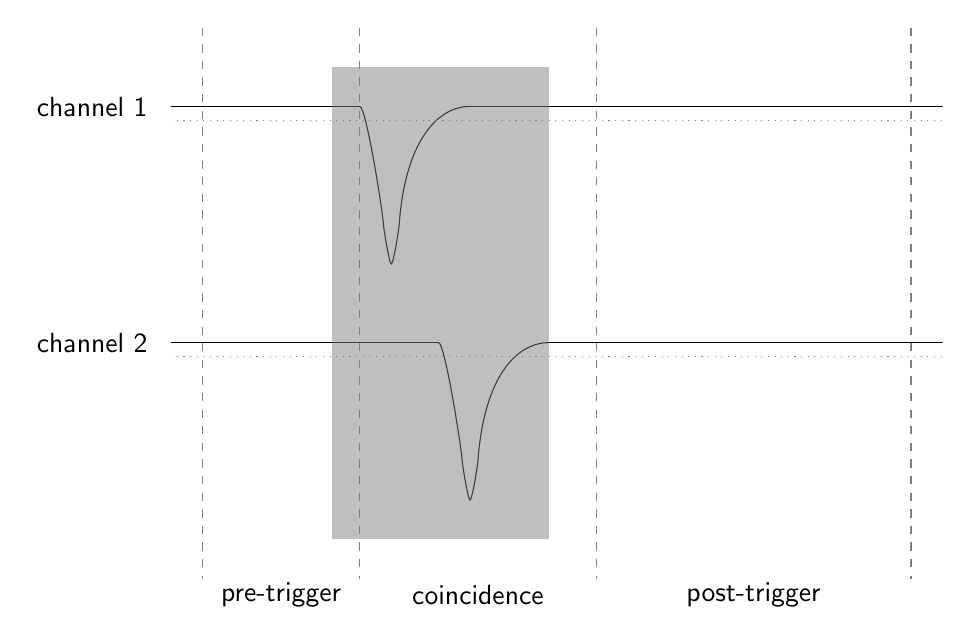
\begin{tikzpicture}[x=2cm,font={\sffamily}]

\node at (-1.7, 0) {channel 1};
\node at (-1.7, -3cm) {channel 2};

\node at (-.5, -6.2) {pre-trigger};
\node at (.75, -6.2) {coincidence};
\node at (2.5, -6.2) {post-trigger};

\clip (-1.2, 1) rectangle (3.7, -6);

\pulse
\begin{scope}[yshift=-3cm,xshift=1cm]
\pulse;
\end{scope}

% Time windows
\draw[gray,dashed] (-1, 1) -- +(0, -7);
\draw[gray,dashed] (0, 1) -- +(0, -7);
\draw[gray,dashed] (1.5, 1) -- +(0, -7);
\draw[gray,dashed] (3.5, 1) -- +(0, -7);

% Reduction Threshold
\draw[gray,dotted] (-1.5, 0 - 5pt) -- +(20, 0);
\draw[gray,dotted,yshift=-3cm] (-1.5, 0 - 5pt) -- +(20, 0);

% Data window
\path[fill,gray,opacity=.5] (0 - 10pt, 0.5) rectangle (2.4cm, -5.5);

\end{tikzpicture}

\caption{\captitle{\daq time windows.} A schematic representation of an
event.  Dashed vertical lines: the pre-trigger (\SI{1}{\micro\second}),
coincidence (\SI{1.5}{\micro\second}) and post-trigger
(\SI{3.5}{\micro\second}) windows.  Dotted horizontal line: the data
reduction threshold (\SI{20}{\adc}).  Shaded area: the data-reduction
window. Data outside this window will not be stored.}
\label{fig:daq-time-windows}
\end{figure}
The buffer size is sufficient to hold
\SI{30}{\micro\second} of data. The default measurement time for \hisparc is
\SI{6}{\micro\second}: the pre-trigger is \SI{1}{\micro\second}, the coincidence
window is \SI{1.5}{\micro\second} and the post-trigger is
\SI{3.5}{\micro\second}. In this configuration, the buffer can hold 5 events.
The buffer is capable of continuously storing event data, eliminating dead time.
Events do not overlap. Particles are either observed within the previous event
(if observed before the end of the post-trigger window) or are part of a new
event. \figref{fig:dead-time} shows the time between triggers for a large set of
events. There are no triggers for intervals shorter than \SI{6}{\micro\second},
since events do not overlap. For intervals longer than \SI{6}{\micro\second},
events are observed. No dead time is observed.

\begin{figure}
\centering
{\pgfkeys{/artist/width/.initial=.45\linewidth}
% \usepackage{tikz}
% \usetikzlibrary{arrows}
% \usepackage{pgfplots}
% \pgfplotsset{compat=1.3}
% \usepackage[detect-family]{siunitx}
% \usepackage[eulergreek]{sansmath}
% \sisetup{text-sf=\sansmath}
% \usepackage{relsize}
%
\pgfkeysifdefined{/artist/width}
    {\pgfkeysgetvalue{/artist/width}{\defaultwidth}}
    {\def\defaultwidth{ .4\linewidth }}
%
%
\begin{sansmath}
\begin{tikzpicture}[
        font=\sffamily,
        every pin/.style={inner sep=2pt, font={\sffamily\smaller}},
        every label/.style={inner sep=2pt, font={\sffamily\smaller}},
        every pin edge/.style={<-, >=stealth', shorten <=2pt},
        pin distance=2.5ex,
    ]
    \begin{axis}[
            width=\defaultwidth,
            %
            title={  },
            %
            xlabel={ Time between triggers [\si{\milli\second}] },
            ylabel={ Number of events },
            %
            xmin={ 0 },
            xmax={ 1000 },
            ymin={  },
            ymax={  },
            %
            xtick={  },
            ytick={  },
            %
            tick align=outside,
            max space between ticks=40,
            every tick/.style={},
        ]

        

        
            
            % Draw series plot
            \addplot[no markers,solid,const plot] coordinates {
                (0.0, 147287)
                (20.0, 146066)
                (40.0, 144154)
                (60.0, 142272)
                (80.0, 142025)
                (100.0, 139574)
                (120.0, 137249)
                (140.0, 136536)
                (160.0, 134312)
                (180.0, 133683)
                (200.0, 131668)
                (220.0, 130560)
                (240.0, 128917)
                (260.0, 127331)
                (280.0, 126711)
                (300.0, 125040)
                (320.0, 123828)
                (340.0, 121961)
                (360.0, 120293)
                (380.0, 119455)
                (400.0, 118819)
                (420.0, 117058)
                (440.0, 115814)
                (460.0, 114589)
                (480.0, 112883)
                (500.0, 112432)
                (520.0, 110374)
                (540.0, 109437)
                (560.0, 108296)
                (580.0, 107056)
                (600.0, 105249)
                (620.0, 104967)
                (640.0, 102935)
                (660.0, 102781)
                (680.0, 101053)
                (700.0, 100435)
                (720.0, 99071)
                (740.0, 98205)
                (760.0, 97291)
                (780.0, 96302)
                (800.0, 94444)
                (820.0, 93854)
                (840.0, 92580)
                (860.0, 92052)
                (880.0, 91245)
                (900.0, 90415)
                (920.0, 88733)
                (940.0, 88287)
                (960.0, 87065)
                (980.0, 86228)
                (1000.0, 86228)
            };
        

        

        

        
    \end{axis}
\end{tikzpicture}
\end{sansmath}
% \usepackage{tikz}
% \usetikzlibrary{arrows}
% \usepackage{pgfplots}
% \pgfplotsset{compat=1.3}
% \usepackage[detect-family]{siunitx}
% \usepackage[eulergreek]{sansmath}
% \sisetup{text-sf=\sansmath}
% \usepackage{relsize}
%
\pgfkeysifdefined{/artist/width}
    {\pgfkeysgetvalue{/artist/width}{\defaultwidth}}
    {\def\defaultwidth{ .4\linewidth }}
%
%
\begin{sansmath}
\begin{tikzpicture}[
        font=\sffamily,
        every pin/.style={inner sep=2pt, font={\sffamily\smaller}},
        every label/.style={inner sep=2pt, font={\sffamily\smaller}},
        every pin edge/.style={<-, >=stealth', shorten <=2pt},
        pin distance=2.5ex,
    ]
    \begin{axis}[
            width=\defaultwidth,
            %
            title={  },
            %
            xlabel={ Time between triggers [\si{\micro\second}] },
            ylabel={ Number of events },
            %
            xmin={ 0 },
            xmax={ 100 },
            ymin={  },
            ymax={  },
            %
            xtick={  },
            ytick={  },
            %
            tick align=outside,
            max space between ticks=40,
            every tick/.style={},
        ]

        

        
            
            % Draw series plot
            \addplot[no markers,solid,const plot] coordinates {
                (0.0, 0)
                (2.0, 0)
                (4.0, 15)
                (6.0, 27)
                (8.0, 20)
                (10.0, 20)
                (12.0, 18)
                (14.0, 15)
                (16.0, 14)
                (18.0, 25)
                (20.0, 17)
                (22.0, 20)
                (24.0, 18)
                (26.0, 22)
                (28.0, 22)
                (30.0, 21)
                (32.0, 20)
                (34.0, 23)
                (36.0, 18)
                (38.0, 29)
                (40.0, 15)
                (42.0, 24)
                (44.0, 17)
                (46.0, 19)
                (48.0, 13)
                (50.0, 21)
                (52.0, 17)
                (54.0, 21)
                (56.0, 15)
                (58.0, 16)
                (60.0, 18)
                (62.0, 19)
                (64.0, 25)
                (66.0, 24)
                (68.0, 14)
                (70.0, 23)
                (72.0, 22)
                (74.0, 24)
                (76.0, 24)
                (78.0, 22)
                (80.0, 23)
                (82.0, 21)
                (84.0, 22)
                (86.0, 28)
                (88.0, 26)
                (90.0, 22)
                (92.0, 29)
                (94.0, 22)
                (96.0, 20)
                (98.0, 23)
                (100.0, 23)
            };
        

        

        

        
    \end{axis}
\end{tikzpicture}
\end{sansmath}
}
\caption{Time between triggers. The recorded length of an event is
\SI{6}{\micro\second}. There are no triggers for intervals shorter than this
value, since events do not overlap. For all intervals longer than
\SI{6}{\micro\second}, events are observed. Since the GPS timestamp is
determined when the trigger condition is fulfilled, and not at the start of
the coincidence window, it is possible to observe events with a time
difference less than \SI{6}{\micro\second}. Indeed, 15 events occur in the
\SIrange{4}{6}{\micro\second} interval. There is no significant dead time.}
\label{fig:dead-time}
\end{figure}


\subsection{GPS Timestamp}
\label{sec:gps-timing}

The \hisparc electronics contains a dedicated high accuracy GPS board, which
provides an accurate timestamp to the data \cite{trimble}.  The GPS provides
several modes of operation. In \emph{self-survey mode}, the antenna's position
is determined by averaging over many \emph{fixes}\footnote{In \SI{24}{\hour},
\num{86400} fixes are collected.}. For each fix, the GPS operates in \emph{full
position mode}. The signals from the satellites are used to calculate both
the current time and the position of the antenna. Once the position is
accurately known, at the end of the self-survey, the GPS switches to
\emph{overdetermined clock mode}. Since the position is static, the
equations can be solved for current time only. Using many satellites, the
system of equations is overdetermined and this results in a more accurate
measurement of the GPS time.

The \hisparc \SI{200}{\mega\hertz} clock is disciplined with the GPS
pulse-per-second (PPS) signal.  The PPS signal and the clock tick counts
are combined into a trigger time which is determined at
\SI{5}{\nano\second} intervals.  By inspecting the PMT signal the trigger time
is adjusted to \SI{2.5}{\nano\second} intervals.  The trigger time is then
corrected by taking the GPS-provided quantization error into account, and
is rounded to the nearest nanosecond.

The GPS can report time either in UTC or GPS time.
Both these times are essentially equal to \emph{international atomic time}
(TAI), up to a difference in \emph{leap seconds}.  Leap seconds are introduced
to better match the UTC clock to \emph{mean solar time}, determined by the
Earth's rotation.  Since the rotation of the Earth is not constant in time, and
is continuously slowing down, leap seconds need to be introduced to synchronize
UTC to mean solar time.  The introduction of leap seconds, however, means that
UTC is periodically adjusted and is not strictly monotonically increasing.  GPS
time, however, is directly based on TAI, and thus maintains the same offset, but
was designed to match UTC in 1980. Since then, GPS time and UTC have diverged.
As of December 31, 2008, the difference between UTC and GPS is \SI{15}{\second},
GPS time being ahead of UTC.  Because the GPS time is both continuous and more
natural for the GPS receiver (UTC has to be calculated, after all necessary
parameters are received from the GPS satellites, which can take several minutes
after startup), all \hisparc stations have their clocks set to GPS
time.

The accuracy of the GPS device is important for the analysis of coincidences
between multiple stations which each have their own GPS device.  To test the
accuracy a pulse generator was used as an external trigger source.  The
trigger was distributed simultaneously to stations 501 and 502, which have a
separation distance of \SI{100}{\meter}.  The two cables used to connect the
triggers had different lengths and the resulting time delay has been measured
and corrected for.
The trigger period has been set to \SI{0.251}{\second}, ensuring a trigger rate
of approximately \SI{4}{\hertz}, while sampling the timing accuracy over the
full subsecond range.  The results of a \SI{24}{\hour} measurement of the time
differences between both stations are shown in
\figref{fig:gps-timing-distribution}.
\begin{figure}
\centering
% \usepackage{tikz}
% \usetikzlibrary{arrows}
% \usepackage{pgfplots}
% \pgfplotsset{compat=1.3}
% \usepackage[detect-family]{siunitx}
% \usepackage[eulergreek]{sansmath}
% \sisetup{text-sf=\sansmath}
% \usepackage{relsize}
%
\pgfkeysifdefined{/artist/width}
    {\pgfkeysgetvalue{/artist/width}{\defaultwidth}}
    {\def\defaultwidth{ .67\linewidth }}
%
%
\begin{sansmath}
\begin{tikzpicture}[
        font=\sffamily,
        every pin/.style={inner sep=2pt, font={\sffamily\smaller}},
        every label/.style={inner sep=2pt, font={\sffamily\smaller}},
        every pin edge/.style={<-, >=stealth', shorten <=2pt},
        pin distance=2.5ex,
    ]
    \begin{axis}[
            width=\defaultwidth,
            %
            title={  },
            %
            xlabel={ Time difference [\si{\nano\second}] },
            ylabel={ Count },
            %
            xmin={ 5 },
            xmax={ 30 },
            ymin={ 0 },
            ymax={  },
            %
            xtick={  },
            ytick={  },
            %
            tick align=outside,
            max space between ticks=40,
            every tick/.style={},
        ]

        

        
            \addplot[no markers,solid,const plot] coordinates {
                (-50.5, 0)
                (-49.5, 0)
                (-48.5, 0)
                (-47.5, 0)
                (-46.5, 0)
                (-45.5, 0)
                (-44.5, 0)
                (-43.5, 0)
                (-42.5, 0)
                (-41.5, 0)
                (-40.5, 0)
                (-39.5, 0)
                (-38.5, 0)
                (-37.5, 0)
                (-36.5, 0)
                (-35.5, 0)
                (-34.5, 0)
                (-33.5, 0)
                (-32.5, 0)
                (-31.5, 0)
                (-30.5, 0)
                (-29.5, 0)
                (-28.5, 0)
                (-27.5, 0)
                (-26.5, 0)
                (-25.5, 0)
                (-24.5, 0)
                (-23.5, 0)
                (-22.5, 0)
                (-21.5, 0)
                (-20.5, 0)
                (-19.5, 0)
                (-18.5, 0)
                (-17.5, 0)
                (-16.5, 0)
                (-15.5, 0)
                (-14.5, 0)
                (-13.5, 0)
                (-12.5, 0)
                (-11.5, 0)
                (-10.5, 0)
                (-9.5, 0)
                (-8.5, 0)
                (-7.5, 0)
                (-6.5, 0)
                (-5.5, 0)
                (-4.5, 0)
                (-3.5, 0)
                (-2.5, 0)
                (-1.5, 0)
                (-0.5, 1)
                (0.5, 0)
                (1.5, 1)
                (2.5, 4)
                (3.5, 7)
                (4.5, 13)
                (5.5, 50)
                (6.5, 117)
                (7.5, 217)
                (8.5, 510)
                (9.5, 1197)
                (10.5, 2747)
                (11.5, 5535)
                (12.5, 10225)
                (13.5, 17511)
                (14.5, 25764)
                (15.5, 34058)
                (16.5, 41268)
                (17.5, 44485)
                (18.5, 43584)
                (19.5, 38311)
                (20.5, 30356)
                (21.5, 21202)
                (22.5, 13175)
                (23.5, 7231)
                (24.5, 3548)
                (25.5, 1538)
                (26.5, 571)
                (27.5, 198)
                (28.5, 59)
                (29.5, 22)
                (30.5, 7)
                (31.5, 4)
                (32.5, 1)
                (33.5, 1)
                (34.5, 0)
                (35.5, 0)
                (36.5, 2)
                (37.5, 1)
                (38.5, 2)
                (39.5, 0)
                (40.5, 0)
                (41.5, 1)
                (42.5, 0)
                (43.5, 0)
                (44.5, 0)
                (45.5, 0)
                (46.5, 0)
                (47.5, 0)
                (48.5, 0)
                (49.5, 0)
            };
        
            \addplot[no markers,gray] coordinates {
                (-50.0, 1.93973901404e-104)
                (-49.8998998999, 4.03094552394e-104)
                (-49.7997997998, 8.36766470632e-104)
                (-49.6996996997, 1.73514320133e-103)
                (-49.5995995996, 3.59418219829e-103)
                (-49.4994994995, 7.43701345743e-103)
                (-49.3993993994, 1.53720135457e-102)
                (-49.2992992993, 3.17392501533e-102)
                (-49.1991991992, 6.5463056462e-102)
                (-49.0990990991, 1.34874425427e-101)
                (-48.998998999, 2.77585418611e-101)
                (-48.8988988989, 5.70686242764e-101)
                (-48.7987987988, 1.17201149216e-100)
                (-48.6986986987, 2.40436307463e-100)
                (-48.5985985986, 4.92721986069e-100)
                (-48.4984984985, 1.00864315663e-99)
                (-48.3983983984, 2.06256129418e-99)
                (-48.2982982983, 4.21317883122e-99)
                (-48.1981981982, 8.5969942434e-99)
                (-48.0980980981, 1.75233482115e-98)
                (-47.997997998, 3.56797053108e-98)
                (-47.8978978979, 7.25703368718e-98)
                (-47.7977977978, 1.47445231619e-97)
                (-47.6976976977, 2.99251294383e-97)
                (-47.5975975976, 6.06701481925e-97)
                (-47.4974974975, 1.22870545541e-96)
                (-47.3973973974, 2.48573158044e-96)
                (-47.2972972973, 5.02336095849e-96)
                (-47.1971971972, 1.01407074652e-95)
                (-47.0970970971, 2.04491770828e-95)
                (-46.996996997, 4.11924031835e-95)
                (-46.8968968969, 8.28880907328e-95)
                (-46.7967967968, 1.66609919736e-94)
                (-46.6966966967, 3.34536328953e-94)
                (-46.5965965966, 6.7099522737e-94)
                (-46.4964964965, 1.34440242775e-93)
                (-46.3963963964, 2.69074695565e-93)
                (-46.2962962963, 5.37960191755e-93)
                (-46.1961961962, 1.07438796408e-92)
                (-46.0960960961, 2.14341290824e-92)
                (-45.995995996, 4.27153787768e-92)
                (-45.8958958959, 8.503474122e-92)
                (-45.7957957958, 1.69099467345e-91)
                (-45.6956956957, 3.35909121719e-91)
                (-45.5955955956, 6.66553583854e-91)
                (-45.4954954955, 1.32124102697e-90)
                (-45.3953953954, 2.61615063481e-90)
                (-45.2952952953, 5.17460441587e-90)
                (-45.1951951952, 1.02241044043e-89)
                (-45.0950950951, 2.01793470336e-89)
                (-44.994994995, 3.97853016554e-89)
                (-44.8948948949, 7.83559380105e-89)
                (-44.7947947948, 1.5415403088e-88)
                (-44.6946946947, 3.02950427207e-88)
                (-44.5945945946, 5.94732902646e-88)
                (-44.4944944945, 1.1662887192e-87)
                (-44.3943943944, 2.28467219764e-87)
                (-44.2942942943, 4.47069900175e-87)
                (-44.1941941942, 8.73897864658e-87)
                (-44.0940940941, 1.70639526675e-86)
                (-43.993993994, 3.32837545008e-86)
                (-43.8938938939, 6.48513012768e-86)
                (-43.7937937938, 1.26223085531e-85)
                (-43.6936936937, 2.45410196055e-85)
                (-43.5935935936, 4.76628629124e-85)
                (-43.4934934935, 9.24701070453e-85)
                (-43.3933933934, 1.79207552387e-84)
                (-43.2932932933, 3.46932486543e-84)
                (-43.1931931932, 6.70914753156e-84)
                (-43.0930930931, 1.29605498761e-83)
                (-42.992992993, 2.50099731831e-83)
                (-42.8928928929, 4.82099562133e-83)
                (-42.7927927928, 9.28311991759e-83)
                (-42.6926926927, 1.7856029585e-82)
                (-42.5925925926, 3.43091173714e-82)
                (-42.4924924925, 6.58518389012e-82)
                (-42.3923923924, 1.2625831268e-81)
                (-42.2922922923, 2.4181640911e-81)
                (-42.1921921922, 4.62642223995e-81)
                (-42.0920920921, 8.84175504517e-81)
                (-41.991991992, 1.6879726417e-80)
                (-41.8918918919, 3.2190375333e-80)
                (-41.7917917918, 6.13225760115e-80)
                (-41.6916916917, 1.16693980073e-79)
                (-41.5915915916, 2.21824865819e-79)
                (-41.4914914915, 4.21216829668e-79)
                (-41.3913913914, 7.98978173135e-79)
                (-41.2912912913, 1.51390222753e-78)
                (-41.1911911912, 2.86546067978e-78)
                (-41.0910910911, 5.41782273611e-78)
                (-40.990990991, 1.02326670197e-77)
                (-40.8908908909, 1.93057467665e-77)
                (-40.7907907908, 3.63846399038e-77)
                (-40.6906906907, 6.84988482967e-77)
                (-40.5905905906, 1.28819666544e-76)
                (-40.4904904905, 2.41999675881e-76)
                (-40.3903903904, 4.54130960038e-76)
                (-40.2902902903, 8.51297091337e-76)
                (-40.1901901902, 1.59409757474e-75)
                (-40.0900900901, 2.98182646641e-75)
                (-39.98998999, 5.57164634164e-75)
                (-39.8898898899, 1.03996430059e-74)
                (-39.7897897898, 1.9390411838e-74)
                (-39.6896896897, 3.61151437521e-74)
                (-39.5895895896, 6.71932078434e-74)
                (-39.4894894895, 1.24880639741e-73)
                (-39.3893893894, 2.31845444702e-73)
                (-39.2892892893, 4.29967601562e-73)
                (-39.1891891892, 7.96538203061e-73)
                (-39.0890890891, 1.47404655548e-72)
                (-38.988988989, 2.72489331303e-72)
                (-38.8888888889, 5.03177854067e-72)
                (-38.7887887888, 9.28169400614e-72)
                (-38.6886886887, 1.71027791414e-71)
                (-38.5885885886, 3.14803709167e-71)
                (-38.4884884885, 5.78824235353e-71)
                (-38.3883883884, 1.06313223202e-70)
                (-38.2882882883, 1.95057016178e-70)
                (-38.1881881882, 3.57494677473e-70)
                (-38.0880880881, 6.54502480203e-70)
                (-37.987987988, 1.19697953606e-69)
                (-37.8878878879, 2.18673354539e-69)
                (-37.7877877878, 3.99060480817e-69)
                (-37.6876876877, 7.27470335174e-69)
                (-37.5875875876, 1.32472449813e-68)
                (-37.4874874875, 2.40973652193e-68)
                (-37.3873873874, 4.37872090443e-68)
                (-37.2872872873, 7.94801506922e-68)
                (-37.1871871872, 1.44113216614e-67)
                (-37.0870870871, 2.61025330477e-67)
                (-36.986986987, 4.72275274829e-67)
                (-36.8868868869, 8.53574588118e-67)
                (-36.7867867868, 1.54106677594e-66)
                (-36.6866866867, 2.77929822787e-66)
                (-36.5865865866, 5.00705723854e-66)
                (-36.4864864865, 9.01080672079e-66)
                (-36.3863863864, 1.61986381869e-65)
                (-36.2862862863, 2.90888832468e-65)
                (-36.1861861862, 5.21806283603e-65)
                (-36.0860860861, 9.3502941439e-65)
                (-35.985985986, 1.67368974254e-64)
                (-35.8858858859, 2.99266668066e-64)
                (-35.7857857858, 5.34534148141e-64)
                (-35.6856856857, 9.53731823154e-64)
                (-35.5855855856, 1.6998508067e-63)
                (-35.4854854855, 3.0264189666e-63)
                (-35.3853853854, 5.38246242835e-63)
                (-35.2852852853, 9.56239493633e-63)
                (-35.1851851852, 1.6970164755e-62)
                (-35.0850850851, 3.00842475384e-62)
                (-34.984984985, 5.32753069807e-62)
                (-34.8848848849, 9.42424311268e-62)
                (-34.7847847848, 1.66533156373e-61)
                (-34.6846846847, 2.93960284299e-61)
                (-34.5845845846, 5.18334739204e-61)
                (-34.4844844845, 9.12989298507e-61)
                (-34.3843843844, 1.60640397497e-60)
                (-34.2842842843, 2.82343351616e-60)
                (-34.1841841842, 4.957172983e-60)
                (-34.0840840841, 8.69409327043e-60)
                (-33.983983984, 1.52316947799e-59)
                (-33.8838838839, 2.66566687145e-59)
                (-33.7837837838, 4.66012143053e-59)
                (-33.6836836837, 8.13808655812e-59)
                (-33.5835835836, 1.41964935269e-58)
                (-33.4834834835, 2.47385126662e-58)
                (-33.3833833834, 4.30625550597e-58)
                (-33.2832832833, 7.48789449195e-58)
                (-33.1831831832, 1.30062875316e-57)
                (-33.0830830831, 2.25673569286e-57)
                (-32.982982983, 3.91148579571e-57)
                (-32.8828828829, 6.77230532463e-57)
                (-32.7827827828, 1.17129156196e-56)
                (-32.6826826827, 2.0236118416e-56)
                (-32.5825825826, 3.49239310573e-56)
                (-32.4824824825, 6.02077981433e-56)
                (-32.3823823824, 1.03685035395e-55)
                (-32.2822822823, 1.78366433367e-55)
                (-32.1821821822, 3.06509464086e-55)
                (-32.0820820821, 5.26148530686e-55)
                (-31.981981982, 9.02207738221e-55)
                (-31.8818818819, 1.54539123992e-54)
                (-31.7817817818, 2.64425940139e-54)
                (-31.6816816817, 4.51963518299e-54)
                (-31.5815815816, 7.71678529463e-54)
                (-31.4814814815, 1.31614326526e-53)
                (-31.3813813814, 2.2423511686e-53)
                (-31.2812812813, 3.81625864704e-53)
                (-31.1811811812, 6.4879230164e-53)
                (-31.0810810811, 1.10181146546e-52)
                (-30.980980981, 1.86914330391e-52)
                (-30.8808808809, 3.16746353458e-52)
                (-30.7807807808, 5.36184630431e-52)
                (-30.6806806807, 9.06673266551e-52)
                (-30.5805805806, 1.53151400652e-51)
                (-30.4804804805, 2.58419241838e-51)
                (-30.3803803804, 4.35574488786e-51)
                (-30.2802802803, 7.33387892277e-51)
                (-30.1801801802, 1.23349884906e-50)
                (-30.0800800801, 2.07241856465e-50)
                (-29.97997998, 3.47816284964e-50)
                (-29.8798798799, 5.83117483144e-50)
                (-29.7797797798, 9.76553241641e-50)
                (-29.6796796797, 1.63368944016e-49)
                (-29.5795795796, 2.73008890714e-49)
                (-29.4794794795, 4.5574067524e-49)
                (-29.3793793794, 7.59963099213e-49)
                (-29.2792792793, 1.26590446451e-48)
                (-29.1791791792, 2.10641078852e-48)
                (-29.0790790791, 3.50121614151e-48)
                (-28.978978979, 5.8133769749e-48)
                (-28.8788788789, 9.64210292269e-48)
                (-28.7787787788, 1.59752900622e-47)
                (-28.6786786787, 2.64398784557e-47)
                (-28.5785785786, 4.37123212094e-47)
                (-28.4784784785, 7.21908235439e-47)
                (-28.3783783784, 1.19095084273e-46)
                (-28.2782782783, 1.96263431807e-46)
                (-28.1781781782, 3.23086382435e-46)
                (-28.0780780781, 5.31289987321e-46)
                (-27.977977978, 8.72726817972e-46)
                (-27.8778778779, 1.43205179008e-45)
                (-27.7777777778, 2.34732292347e-45)
                (-27.6776776777, 3.84344497781e-45)
                (-27.5775775776, 6.28640285789e-45)
                (-27.4774774775, 1.02711119365e-44)
                (-27.3773773774, 1.67635667563e-44)
                (-27.2772772773, 2.73305962737e-44)
                (-27.1771771772, 4.45108100475e-44)
                (-27.0770770771, 7.24128435336e-44)
                (-26.976976977, 1.17679121675e-43)
                (-26.8768768769, 1.91036761529e-43)
                (-26.7767767768, 3.097905666e-43)
                (-26.6766766767, 5.0182598213e-43)
                (-26.5765765766, 8.12029506019e-43)
                (-26.4764764765, 1.3125751856e-42)
                (-26.3763763764, 2.11938707613e-42)
                (-26.2762762763, 3.4184567249e-42)
                (-26.1761761762, 5.50786901747e-42)
                (-26.0760760761, 8.86483861612e-42)
                (-25.975975976, 1.42525238447e-41)
                (-25.8758758759, 2.28900336663e-41)
                (-25.7757757758, 3.67227164411e-41)
                (-25.6756756757, 5.8851410975e-41)
                (-25.5755755756, 9.42133990443e-41)
                (-25.4754754755, 1.5066146227e-40)
                (-25.3753753754, 2.40671905499e-40)
                (-25.2752752753, 3.84045187511e-40)
                (-25.1751751752, 6.12171308123e-40)
                (-25.0750750751, 9.74759164085e-40)
                (-24.974974975, 1.55044153962e-39)
                (-24.8748748749, 2.46346942711e-39)
                (-24.7747747748, 3.9099632076e-39)
                (-24.6746746747, 6.19914617775e-39)
                (-24.5745745746, 9.81803998337e-39)
                (-24.4744744745, 1.5532860009e-38)
                (-24.3743743744, 2.45477545693e-38)
                (-24.2742742743, 3.87530447191e-38)
                (-24.1741741742, 6.11129993792e-38)
                (-24.0740740741, 9.62709109499e-38)
                (-23.973973974, 1.51492201239e-37)
                (-23.8738738739, 2.38132780826e-37)
                (-23.7737737738, 3.73922676391e-37)
                (-23.6736736737, 5.86513666565e-37)
                (-23.5735735736, 9.1898448951e-37)
                (-23.4734734735, 1.43837438154e-36)
                (-23.3733733734, 2.2488961961e-36)
                (-23.2732732733, 3.51237270027e-36)
                (-23.1731731732, 5.47980985002e-36)
                (-23.0730730731, 8.54012243577e-36)
                (-22.972972973, 1.32952472406e-35)
                (-22.8728728729, 2.06758061409e-35)
                (-22.7727727728, 3.21190134812e-35)
                (-22.6726726727, 4.98420224499e-35)
                (-22.5725725726, 7.72614452636e-35)
                (-22.4724724725, 1.19636503507e-34)
                (-22.3723723724, 1.85053928221e-34)
                (-22.2722722723, 2.85934538537e-34)
                (-22.1721721722, 4.41335273467e-34)
                (-22.0720720721, 6.80462778292e-34)
                (-21.971971972, 1.0480302571e-33)
                (-21.8718718719, 1.61241556109e-33)
                (-21.7717717718, 2.47807161487e-33)
                (-21.6716716717, 3.80438480147e-33)
                (-21.5715715716, 5.8342997141e-33)
                (-21.4714714715, 8.93772001351e-33)
                (-21.3713713714, 1.36772400215e-32)
                (-21.2712712713, 2.09075865735e-32)
                (-21.1711711712, 3.19258928516e-32)
                (-21.0710710711, 4.86985367745e-32)
                (-20.970970971, 7.42031745392e-32)
                (-20.8708708709, 1.12943897744e-31)
                (-20.7707707708, 1.7172628301e-31)
                (-20.6706706707, 2.60822156169e-31)
                (-20.5705705706, 3.95718090238e-31)
                (-20.4704704705, 5.99737273208e-31)
                (-20.3703703704, 9.07966634588e-31)
                (-20.2702702703, 1.37313251499e-30)
                (-20.1701701702, 2.07438195194e-30)
                (-20.0700700701, 3.13039190573e-30)
                (-19.96996997, 4.71891778851e-30)
                (-19.8698698699, 7.10591197303e-30)
                (-19.7697697698, 1.06888491446e-29)
                (-19.6696696697, 1.60611184473e-29)
                (-19.5695695696, 2.41076198614e-29)
                (-19.4694694695, 3.61465287475e-29)
                (-19.3693693694, 5.41392920107e-29)
                (-19.2692692693, 8.1001350501e-29)
                (-19.1691691692, 1.21061391088e-28)
                (-19.0690690691, 1.80739373617e-28)
                (-18.968968969, 2.69546438742e-28)
                (-18.8688688689, 4.01557864859e-28)
                (-18.7687687688, 5.97580458342e-28)
                (-18.6686686687, 8.88338225483e-28)
                (-18.5685685686, 1.31914952754e-27)
                (-18.4684684685, 1.95678637071e-27)
                (-18.3683683684, 2.89952271858e-27)
                (-18.2682682683, 4.29183808867e-27)
                (-18.1681681682, 6.34590923353e-27)
                (-18.0680680681, 9.37298873373e-27)
                (-17.967967968, 1.38291678098e-26)
                (-17.8678678679, 2.03820428739e-26)
                (-17.7677677678, 3.00077261373e-26)
                (-17.6676676677, 4.41318544364e-26)
                (-17.5675675676, 6.48343228178e-26)
                (-17.4674674675, 9.51462100453e-26)
                (-17.3673673674, 1.39479930082e-25)
                (-17.2672672673, 2.04251691064e-25)
                (-17.1671671672, 2.98781231769e-25)
                (-17.0670670671, 4.36590899141e-25)
                (-16.966966967, 6.37279218073e-25)
                (-16.8668668669, 9.29219995277e-25)
                (-16.7667667668, 1.35344636328e-24)
                (-16.6666666667, 1.96923372572e-24)
                (-16.5665665666, 2.86211574759e-24)
                (-16.4664664665, 4.15538084972e-24)
                (-16.3663663664, 6.02654199717e-24)
                (-16.2662662663, 8.730904812e-24)
                (-16.1661661662, 1.26352556078e-23)
                (-16.0660660661, 1.82659608821e-23)
                (-15.965965966, 2.63775665295e-23)
                (-15.8658658659, 3.80505241454e-23)
                (-15.7657657658, 5.48302558776e-23)
                (-15.6656656657, 7.89248225833e-23)
                (-15.5655655656, 1.1348557661e-22)
                (-15.4654654655, 1.63005191195e-22)
                (-15.3653653654, 2.33881523974e-22)
                (-15.2652652653, 3.35215511927e-22)
                (-15.1651651652, 4.79938966462e-22)
                (-15.0650650651, 6.86406882221e-22)
                (-14.964964965, 9.80643060193e-22)
                (-14.8648648649, 1.39950354168e-21)
                (-14.7647647648, 1.99512796979e-21)
                (-14.6646646647, 2.84119619822e-21)
                (-14.5645645646, 4.04171238634e-21)
                (-14.4644644645, 5.7433237537e-21)
                (-14.3643643644, 8.1525768995e-21)
                (-14.2642642643, 1.15600635685e-20)
                (-14.1641641642, 1.63741684214e-20)
                (-14.0640640641, 2.31681841585e-20)
                (-13.963963964, 3.27460147222e-20)
                (-13.8638638639, 4.62336968939e-20)
                (-13.7637637638, 6.520674218e-20)
                (-13.6636636637, 9.18671189669e-20)
                (-13.5635635636, 1.29288948475e-19)
                (-13.4634634635, 1.81759208346e-19)
                (-13.3633633634, 2.55249649408e-19)
                (-13.2632632633, 3.58069721638e-19)
                (-13.1631631632, 5.01768918165e-19)
                (-13.0630630631, 7.02382407442e-19)
                (-12.962962963, 9.8214861263e-19)
                (-12.8628628629, 1.371874875e-18)
                (-12.7627627628, 1.91419205714e-18)
                (-12.6626626627, 2.66802705915e-18)
                (-12.5625625626, 3.71474205546e-18)
                (-12.4624624625, 5.16655203642e-18)
                (-12.3623623624, 7.17805308442e-18)
                (-12.2622622623, 9.96199309348e-18)
                (-12.1621621622, 1.38108217304e-17)
                (-12.0620620621, 1.91261040982e-17)
                (-11.961961962, 2.64586221065e-17)
                (-11.8618618619, 3.65629850209e-17)
                (-11.7617617618, 5.04719144331e-17)
                (-11.6616616617, 6.9597177033e-17)
                (-11.5615615616, 9.58665686905e-17)
                (-11.4614614615, 1.31909615543e-16)
                (-11.3613613614, 1.8130903174e-16)
                (-11.2612612613, 2.48940831178e-16)
                (-11.1611611612, 3.414338259e-16)
                (-11.0610610611, 4.67789712191e-16)
                (-10.960960961, 6.40218914786e-16)
                (-10.8608608609, 8.75265978891e-16)
                (-10.7607607608, 1.19532308696e-15)
                (-10.6606606607, 1.63066323638e-15)
                (-10.5605605606, 2.22216838729e-15)
                (-10.4604604605, 3.02498595495e-15)
                (-10.3603603604, 4.11342395336e-15)
                (-10.2602602603, 5.58749690413e-15)
                (-10.1601601602, 7.58166918856e-15)
                (-10.0600600601, 1.02765201685e-14)
                (-9.95995995996, 1.39142896446e-14)
                (-9.85985985986, 1.8819570718e-14)
                (-9.75975975976, 2.54268229271e-14)
                (-9.65965965966, 3.43169116871e-14)
                (-9.55955955956, 4.62655796975e-14)
                (-9.45945945946, 6.23076729776e-14)
                (-9.35935935936, 8.38221446036e-14)
                (-9.25925925926, 1.12644428778e-13)
                (-9.15915915916, 1.5121482757e-13)
                (-9.05905905906, 2.02774226168e-13)
                (-8.95895895896, 2.71621935446e-13)
                (-8.85885885886, 3.6345499252e-13)
                (-8.75875875876, 4.85814139629e-13)
                (-8.65865865866, 6.48669346476e-13)
                (-8.55855855856, 8.65187652108e-13)
                (-8.45845845846, 1.15273893563e-12)
                (-8.35835835836, 1.53421182172e-12)
                (-8.25825825826, 2.03973336472e-12)
                (-8.15815815816, 2.7089138119e-12)
                (-8.05805805806, 3.59377338304e-12)
                (-7.95795795796, 4.76255386554e-12)
                (-7.85785785786, 6.30467677329e-12)
                (-7.75775775776, 8.33718549507e-12)
                (-7.65765765766, 1.10131058913e-11)
                (-7.55755755756, 1.45322840591e-11)
                (-7.45745745746, 1.91554189214e-11)
                (-7.35735735736, 2.52222103208e-11)
                (-7.25725725726, 3.3174802343e-11)
                (-7.15715715716, 4.35880316707e-11)
                (-7.05705705706, 5.72084108746e-11)
                (-6.95695695696, 7.50043105274e-11)
                (-6.85685685686, 9.82304819427e-11)
                (-6.75675675676, 1.28510921882e-10)
                (-6.65665665666, 1.67945169062e-10)
                (-6.55655655656, 2.19244498965e-10)
                (-6.45645645646, 2.85906222447e-10)
                (-6.35635635636, 3.72436487504e-10)
                (-6.25625625626, 4.84634747838e-10)
                (-6.15615615616, 6.29956540472e-10)
                (-6.05605605606, 8.17975586574e-10)
                (-5.95595595596, 1.06097171747e-09)
                (-5.85585585586, 1.37467800743e-09)
                (-5.75575575576, 1.77922910851e-09)
                (-5.65565565566, 2.30036355333e-09)
                (-5.55555555556, 2.9709462431e-09)
                (-5.45545545546, 3.8328941148e-09)
                (-5.35535535536, 4.93960887986e-09)
                (-5.25525525526, 6.35904672507e-09)
                (-5.15515515516, 8.17758716835e-09)
                (-5.05505505506, 1.05049033441e-08)
                (-4.95495495495, 1.34800856635e-08)
                (-4.85485485485, 1.72793322718e-08)
                (-4.75475475475, 2.21255957081e-08)
                (-4.65465465465, 2.83006689745e-08)
                (-4.55455455455, 3.61603098559e-08)
                (-4.45445445445, 4.61531447055e-08)
                (-4.35435435435, 5.88442679702e-08)
                (-4.25425425425, 7.49446686997e-08)
                (-4.15415415415, 9.53478789122e-08)
                (-4.05405405405, 1.21175561565e-07)
                (-3.95395395395, 1.53834150794e-07)
                (-3.85385385385, 1.95085139473e-07)
                (-3.75375375375, 2.47132197582e-07)
                (-3.65365365365, 3.12729021738e-07)
                (-3.55355355355, 3.95312688393e-07)
                (-3.45345345345, 4.9916834278e-07)
                (-3.35335335335, 6.29632341408e-07)
                (-3.25325325325, 7.93342523686e-07)
                (-3.15315315315, 9.98546173313e-07)
                (-3.05305305305, 1.25547850795e-06)
                (-2.95295295295, 1.57682728451e-06)
                (-2.85285285285, 1.97830242001e-06)
                (-2.75275275275, 2.47933351433e-06)
                (-2.65265265265, 3.10392295235e-06)
                (-2.55255255255, 3.88168801212e-06)
                (-2.45245245245, 4.84913229669e-06)
                (-2.35235235235, 6.0511950533e-06)
                (-2.25225225225, 7.54313679892e-06)
                (-2.15215215215, 9.39283143249e-06)
                (-2.05205205205, 1.16835490303e-05)
                (-1.95195195195, 1.45173302004e-05)
                (-1.85185185185, 1.80190726938e-05)
                (-1.75175175175, 2.23414744892e-05)
                (-1.65165165165, 2.76710054388e-05)
                (-1.55155155155, 3.42351125381e-05)
                (-1.45145145145, 4.23109028434e-05)
                (-1.35135135135, 5.22355940242e-05)
                (-1.25125125125, 6.44190766864e-05)
                (-1.15115115115, 7.93589962953e-05)
                (-1.05105105105, 9.76588373364e-05)
                (-0.950950950951, 0.000120049580093)
                (-0.850850850851, 0.000147415603161)
                (-0.750750750751, 0.000180825624951)
                (-0.650650650651, 0.000221569617699)
                (-0.550550550551, 0.000271202790979)
                (-0.45045045045, 0.000331597932013)
                (-0.35035035035, 0.000405007611226)
                (-0.25025025025, 0.000494138018048)
                (-0.15015015015, 0.000602236489209)
                (-0.05005005005, 0.000733195135594)
                (0.0500500500501, 0.000891673370669)
                (0.15015015015, 0.00108324260123)
                (0.25025025025, 0.00131455686805)
                (0.35035035035, 0.00159355382937)
                (0.45045045045, 0.00192969117476)
                (0.550550550551, 0.00233422435234)
                (0.650650650651, 0.00282053240196)
                (0.750750750751, 0.00340449972488)
                (0.850850850851, 0.00410496280402)
                (0.950950950951, 0.0049442322339)
                (1.05105105105, 0.00594870194794)
                (1.15115115115, 0.00714955926238)
                (1.25125125125, 0.00858361131582)
                (1.35135135135, 0.0102942456966)
                (1.45145145145, 0.0123325455444)
                (1.55155155155, 0.0147585822206)
                (1.65165165165, 0.0176429117923)
                (1.75175175175, 0.0210683051098)
                (1.85185185185, 0.0251317452092)
                (1.95195195195, 0.0299467301825)
                (2.05205205205, 0.0356459245759)
                (2.15215215215, 0.0423842078396)
                (2.25225225225, 0.0503421744188)
                (2.35235235235, 0.0597301467852)
                (2.45245245245, 0.0707927701264)
                (2.55255255255, 0.0838142655797)
                (2.65265265265, 0.0991244278846)
                (2.75275275275, 0.117105463185)
                (2.85285285285, 0.138199773498)
                (2.95295295295, 0.16291880614)
                (3.05305305305, 0.19185309922)
                (3.15315315315, 0.225683668224)
                (3.25325325325, 0.265194893797)
                (3.35335335335, 0.311289087087)
                (3.45345345345, 0.365002926529)
                (3.55355355355, 0.427525978774)
                (3.65365365365, 0.500221536534)
                (3.75375375375, 0.58465002757)
                (3.85385385385, 0.682595271828)
                (3.95395395395, 0.796093887769)
                (4.05405405405, 0.927468174393)
                (4.15415415415, 1.07936282202)
                (4.25425425425, 1.25478583281)
                (4.35435435435, 1.45715406072)
                (4.45445445445, 1.69034381084)
                (4.55455455455, 1.95874696827)
                (4.65465465465, 2.26733315849)
                (4.75475475475, 2.62171847256)
                (4.85485485485, 3.02824132266)
                (4.95495495495, 3.49404602494)
                (5.05505505506, 4.02717473805)
                (5.15515515516, 4.63666841585)
                (5.25525525526, 5.33267746182)
                (5.35535535536, 6.12658279953)
                (5.45545545546, 7.03112809818)
                (5.55555555556, 8.06056391354)
                (5.65565565566, 9.23080452235)
                (5.75575575576, 10.5595982412)
                (5.85585585586, 12.0667120292)
                (5.95595595596, 13.7741311737)
                (6.05605605606, 15.7062748558)
                (6.15615615616, 17.8902283751)
                (6.25625625626, 20.3559927928)
                (6.35635635636, 23.1367527195)
                (6.45645645646, 26.2691629263)
                (6.55655655656, 29.7936544079)
                (6.65665665666, 33.7547604477)
                (6.75675675676, 38.2014631586)
                (6.85685685686, 43.1875608655)
                (6.95695695696, 48.7720565839)
                (7.05705705706, 55.0195677095)
                (7.15715715716, 62.0007568813)
                (7.25725725726, 69.792783808)
                (7.35735735736, 78.4797776502)
                (7.45745745746, 88.1533293372)
                (7.55755755756, 98.91300296)
                (7.65765765766, 110.866865122)
                (7.75775775776, 124.132030848)
                (7.85785785786, 138.835224345)
                (7.95795795796, 155.113352597)
                (8.05805805806, 173.114089407)
                (8.15815815816, 192.996467158)
                (8.25825825826, 214.931473161)
                (8.35835835836, 239.102647085)
                (8.45845845846, 265.706675501)
                (8.55855855856, 294.953979206)
                (8.65865865866, 327.06928851)
                (8.75875875876, 362.29220124)
                (8.85885885886, 400.877717792)
                (8.95895895896, 443.096747088)
                (9.05905905906, 489.236576895)
                (9.15915915916, 539.60130151)
                (9.25925925926, 594.512199449)
                (9.35935935936, 654.308053369)
                (9.45945945946, 719.345404115)
                (9.55955955956, 789.998730488)
                (9.65965965966, 866.660546041)
                (9.75975975976, 949.741404019)
                (9.85985985986, 1039.66980138)
                (9.95995995996, 1136.89197275)
                (10.0600600601, 1241.8715652)
                (10.1601601602, 1355.08918472)
                (10.2602602603, 1477.04180538)
                (10.3603603604, 1608.24203268)
                (10.4604604605, 1749.21721255)
                (10.5605605606, 1900.50837818)
                (10.6606606607, 2062.66902741)
                (10.7607607608, 2236.26372398)
                (10.8608608609, 2421.86651679)
                (10.960960961, 2620.05917228)
                (11.0610610611, 2831.42921607)
                (11.1611611612, 3056.56778111)
                (11.2612612613, 3296.06726097)
                (11.3613613614, 3550.51876816)
                (11.4614614615, 3820.5093992)
                (11.5615615616, 4106.61930925)
                (11.6616616617, 4409.41860151)
                (11.7617617618, 4729.46403778)
                (11.8618618619, 5067.29557893)
                (11.961961962, 5423.43276575)
                (12.0620620621, 5798.37095272)
                (12.1621621622, 6192.57740926)
                (12.2622622623, 6606.48730523)
                (12.3623623624, 7040.49959921)
                (12.4624624625, 7494.9728505)
                (12.5625625626, 7970.22097738)
                (12.6626626627, 8466.50898649)
                (12.7627627628, 8984.04869965)
                (12.8628628629, 9522.99450639)
                (12.962962963, 10083.439172)
                (13.0630630631, 10665.4097322)
                (13.1631631632, 11268.8635068)
                (13.2632632633, 11893.6842661)
                (13.3633633634, 12539.6785832)
                (13.4634634635, 13206.5724089)
                (13.5635635636, 13894.007901)
                (13.6636636637, 14601.5405467)
                (13.7637637638, 15328.6366087)
                (13.8638638639, 16074.6709318)
                (13.963963964, 16838.9251413)
                (14.0640640641, 17620.5862645)
                (14.1641641642, 18418.7458061)
                (14.2642642643, 19232.3993036)
                (14.3643643644, 20060.4463895)
                (14.4644644645, 20901.6913811)
                (14.5645645646, 21754.8444192)
                (14.6646646647, 22618.5231705)
                (14.7647647648, 23491.2551062)
                (14.8648648649, 24371.4803663)
                (14.964964965, 25257.5552128)
                (15.0650650651, 26147.7560733)
                (15.1651651652, 27040.284169)
                (15.2652652653, 27933.270719)
                (15.3653653654, 28824.7827075)
                (15.4654654655, 29712.8291943)
                (15.5655655656, 30595.3681456)
                (15.6656656657, 31470.3137579)
                (15.7657657658, 32335.544241)
                (15.8658658659, 33188.9100237)
                (15.965965966, 34028.2423414)
                (16.0660660661, 34851.3621576)
                (16.1661661662, 35656.0893735)
                (16.2662662663, 36440.2522699)
                (16.3663663664, 37201.6971267)
                (16.4664664665, 37938.2979627)
                (16.5665665666, 38647.9663322)
                (16.6666666667, 39328.6611188)
                (16.7667667668, 39978.3982606)
                (16.8668668669, 40595.2603439)
                (16.966966967, 41177.4059991)
                (17.0670670671, 41723.0790364)
                (17.1671671672, 42230.6172573)
                (17.2672672673, 42698.4608788)
                (17.3673673674, 43125.1605137)
                (17.4674674675, 43509.3846463)
                (17.5675675676, 43849.926553)
                (17.6676676677, 44145.7106145)
                (17.7677677678, 44395.7979755)
                (17.8678678679, 44599.3915092)
                (17.967967968, 44755.8400506)
                (18.0680680681, 44864.6418658)
                (18.1681681682, 44925.447333)
                (18.2682682683, 44938.0608143)
                (18.3683683684, 44902.4417046)
                (18.4684684685, 44818.7046491)
                (18.5685685686, 44687.1189285)
                (18.6686686687, 44508.1070166)
                (18.7687687688, 44282.2423199)
                (18.8688688689, 44010.2461182)
                (18.968968969, 43692.9837266)
                (19.0690690691, 43331.4599093)
                (19.1691691692, 42926.8135791)
                (19.2692692693, 42480.3118201)
                (19.3693693694, 41993.3432797)
                (19.4694694695, 41467.4109765)
                (19.5695695696, 40904.1245773)
                (19.6696696697, 40305.1921971)
                (19.7697697698, 39672.411783)
                (19.8698698699, 39007.6621401)
                (19.96996997, 38312.8936639)
                (20.0700700701, 37590.1188416)
                (20.1701701702, 36841.4025877)
                (20.2702702703, 36068.8524786)
                (20.3703703704, 35274.6089487)
                (20.4704704705, 34460.8355138)
                (20.5705705706, 33629.7090814)
                (20.6706706707, 32783.4104081)
                (20.7707707708, 31924.1147622)
                (20.8708708709, 31053.9828452)
                (20.970970971, 30175.1520235)
                (21.0710710711, 29289.7279176)
                (21.1711711712, 28399.7763931)
                (21.2712712713, 27507.3159926)
                (21.3713713714, 26614.310843)
                (21.4714714715, 25722.6640695)
                (21.5715715716, 24834.2117422)
                (21.6716716717, 23950.7173753)
                (21.7717717718, 23073.8669959)
                (21.8718718719, 22205.2647943)
                (21.971971972, 21346.4293619)
                (22.0720720721, 20498.7905189)
                (22.1721721722, 19663.6867304)
                (22.2722722723, 18842.3631042)
                (22.3723723724, 18035.9699586)
                (22.4724724725, 17245.5619483)
                (22.5725725726, 16472.0977286)
                (22.6726726727, 15716.4401382)
                (22.7727727728, 14979.3568757)
                (22.8728728729, 14261.5216451)
                (22.972972973, 13563.5157388)
                (23.0730730731, 12885.8300314)
                (23.1731731732, 12228.8673483)
                (23.2732732733, 11592.9451786)
                (23.3733733734, 10978.2986971)
                (23.4734734735, 10385.0840602)
                (23.5735735736, 9813.38194212)
                (23.6736736737, 9263.20127517)
                (23.7737737738, 8734.4831606)
                (23.8738738739, 8227.10491579)
                (23.973973974, 7740.88422489)
                (24.0740740741, 7275.58336103)
                (24.1741741742, 6830.91344971)
                (24.2742742743, 6406.53874416)
                (24.3743743744, 6002.08088536)
                (24.4744744745, 5617.12312116)
                (24.5745745746, 5251.21446052)
                (24.6746746747, 4903.87374138)
                (24.7747747748, 4574.59359211)
                (24.8748748749, 4262.84426901)
                (24.974974975, 3968.07735404)
                (25.0750750751, 3689.72929931)
                (25.1751751752, 3427.22480659)
                (25.2752752753, 3179.98003244)
                (25.3753753754, 2947.40561112)
                (25.4754754755, 2728.90948962)
                (25.5755755756, 2523.89957071)
                (25.6756756757, 2331.78616164)
                (25.7757757758, 2151.98422786)
                (25.8758758759, 1983.91545225)
                (25.975975976, 1827.01010211)
                (26.0760760761, 1680.70870705)
                (26.1761761762, 1544.46355226)
                (26.2762762763, 1417.73999239)
                (26.3763763764, 1300.01759255)
                (26.4764764765, 1190.79110306)
                (26.5765765766, 1089.57127587)
                (26.6766766767, 995.885530557)
                (26.7767767768, 909.278478541)
                (26.8768768769, 829.312314298)
                (26.976976977, 755.567082583)
                (27.0770770771, 687.640830813)
                (27.1771771772, 625.149655771)
                (27.2772772773, 567.727653719)
                (27.3773773774, 515.026782926)
                (27.4774774775, 466.716647394)
                (27.5775775776, 422.484210346)
                (27.6776776777, 382.033445763)
                (27.7777777778, 345.084935895)
                (27.8778778779, 311.375422339)
                (27.977977978, 280.657317874)
                (28.0780780781, 252.698185831)
                (28.1781781782, 227.280193356)
                (28.2782782783, 204.199544476)
                (28.3783783784, 183.265898447)
                (28.4784784785, 164.301778409)
                (28.5785785786, 147.141974948)
                (28.6786786787, 131.632948721)
                (28.7787787788, 117.632235878)
                (28.8788788789, 105.007859619)
                (28.978978979, 93.6377508139)
                (29.0790790791, 83.4091802638)
                (29.1791791792, 74.2182047863)
                (29.2792792793, 65.9691290154)
                (29.3793793794, 58.573984461)
                (29.4794794795, 51.9520270931)
                (29.5795795796, 46.0292544434)
                (29.6796796797, 40.7379429659)
                (29.7797797798, 36.0162061733)
                (29.8798798799, 31.8075738601)
                (29.97997998, 28.0605925367)
                (30.0800800801, 24.7284470396)
                (30.1801801802, 21.7686031297)
                (30.2802802803, 19.1424707733)
                (30.3803803804, 16.8150876832)
                (30.4804804805, 14.7548226096)
                (30.5805805806, 12.9330977904)
                (30.6806806807, 11.324129908)
                (30.7807807808, 9.90468884882)
                (30.8808808809, 8.65387352209)
                (30.980980981, 7.552903969)
                (31.0810810811, 6.58492897206)
                (31.1811811812, 5.73484836684)
                (31.2812812813, 4.9891492555)
                (31.3813813814, 4.33575532599)
                (31.4814814815, 3.7638884917)
                (31.5815815816, 3.26394208133)
                (31.6816816817, 2.8273648283)
                (31.7817817818, 2.44655493231)
                (31.8818818819, 2.11476349104)
                (31.981981982, 1.82600662816)
                (32.0820820821, 1.57498567347)
                (32.1821821822, 1.35701478157)
                (32.2822822823, 1.16795540711)
                (32.3823823824, 1.00415708647)
                (32.4824824825, 0.86240400751)
                (32.5825825826, 0.739866880737)
                (32.6826826827, 0.634059656086)
                (32.7827827828, 0.542800660099)
                (32.8828828829, 0.464177757512)
                (32.982982983, 0.396517169764)
                (33.0830830831, 0.33835561019)
                (33.1831831832, 0.288415421704)
                (33.2832832833, 0.245582427548)
                (33.3833833834, 0.208886229146)
                (33.4834834835, 0.177482707239)
                (33.5835835836, 0.150638503248)
                (33.6836836837, 0.127717277332)
                (33.7837837838, 0.108167557756)
                (33.8838838839, 0.0915120131189)
                (33.983983984, 0.0773379946801)
                (34.0840840841, 0.0652892105357)
                (34.1841841842, 0.0550584067858)
                (34.2842842843, 0.046380943146)
                (34.3843843844, 0.0390291617503)
                (34.4844844845, 0.03280745823)
                (34.5845845846, 0.0275479735881)
                (34.6846846847, 0.0231068339751)
                (34.7847847848, 0.0193608732825)
                (34.8848848849, 0.0162047805365)
                (34.984984985, 0.013548620477)
                (35.0850850851, 0.0113156814735)
                (35.1851851852, 0.00944061013212)
                (35.2852852853, 0.0078677966132)
                (35.3853853854, 0.00654997886907)
                (35.4854854855, 0.00544703775864)
                (35.5855855856, 0.00452495834161)
                (35.6856856857, 0.00375493563867)
                (35.7857857858, 0.00311260579813)
                (35.8858858859, 0.00257738596609)
                (35.985985986, 0.00213190824597)
                (36.0860860861, 0.00176153498109)
                (36.1861861862, 0.00145394422609)
                (36.2862862863, 0.00119877571102)
                (36.3863863864, 0.000987328867987)
                (36.4864864865, 0.000812305601991)
                (36.5865865866, 0.00066759146231)
                (36.6866866867, 0.000548069724462)
                (36.7867867868, 0.000449463638348)
                (36.8868868869, 0.000368202748886)
                (36.986986987, 0.000301309762103)
                (37.0870870871, 0.000246304922375)
                (37.1871871872, 0.000201125294279)
                (37.2872872873, 0.000164056713219)
                (37.3873873874, 0.000133676489818)
                (37.4874874875, 0.0001088052302)
                (37.5875875876, 8.8466373351e-05)
                (37.6876876877, 7.18522526394e-05)
                (37.7877877878, 5.82956655911e-05)
                (37.8878878879, 4.7246088031e-05)
                (37.987987988, 3.82497989745e-05)
                (38.0880880881, 3.09332941827e-05)
                (38.1881881882, 2.49894615971e-05)
                (38.2882882883, 2.01660732012e-05)
                (38.3883883884, 1.62562171511e-05)
                (38.4884884885, 1.30903529745e-05)
                (38.5885885886, 1.05297227221e-05)
                (38.6886886887, 8.46089344405e-06)
                (38.7887887888, 6.79124234819e-06)
                (38.8888888889, 5.44522643763e-06)
                (38.988988989, 4.36130413065e-06)
                (39.0890890891, 3.48939804743e-06)
                (39.1891891892, 2.78880640545e-06)
                (39.2892892893, 2.22648581946e-06)
                (39.3893893894, 1.77564119539e-06)
                (39.4894894895, 1.41456921906e-06)
                (39.5895895896, 1.12571099423e-06)
                (39.6896896897, 8.94876955099e-07)
                (39.7897897898, 7.10613499479e-07)
                (39.8898898899, 5.63686060686e-07)
                (39.98998999, 4.46657725248e-07)
                (40.0900900901, 3.53546153744e-07)
                (40.1901901902, 2.7954459306e-07)
                (40.2902902903, 2.20795281904e-07)
                (40.3903903904, 1.74205632929e-07)
                (40.4904904905, 1.37299296287e-07)
                (40.5905905906, 1.08095631104e-07)
                (40.6906906907, 8.50122839621e-08)
                (40.7907907908, 6.67865392231e-08)
                (40.8908908909, 5.24119004604e-08)
                (40.990990991, 4.10870147657e-08)
                (41.0910910911, 3.21745870317e-08)
                (41.1911911912, 2.51683698419e-08)
                (41.2912912913, 1.96666733989e-08)
                (41.3913913914, 1.53511330798e-08)
                (41.4914914915, 1.19697114266e-08)
                (41.5915915916, 9.32310631236e-09)
                (41.6916916917, 7.25389567731e-09)
                (41.7917917918, 5.63787817061e-09)
                (41.8918918919, 4.37717369913e-09)
                (41.991991992, 3.39473273113e-09)
                (42.0920920921, 2.62997189277e-09)
                (42.1921921922, 2.03530893445e-09)
                (42.2922922923, 1.57341499072e-09)
                (42.3923923924, 1.2150382243e-09)
                (42.4924924925, 9.37282073031e-10)
                (42.5925925926, 7.22244748853e-10)
                (42.6926926927, 5.55945459929e-10)
                (42.7927927928, 4.27477927902e-10)
                (42.8928928929, 3.28343872389e-10)
                (42.992992993, 2.5192881778e-10)
                (43.0930930931, 1.93090316376e-10)
                (43.1931931932, 1.47834859267e-10)
                (43.2932932933, 1.13064670882e-10)
                (43.3933933934, 8.63795040477e-11)
                (43.4934934935, 6.59216701907e-11)
                (43.5935935936, 5.02550154263e-11)
                (43.6936936937, 3.82705172279e-11)
                (43.7937937938, 2.91127322057e-11)
                (43.8938938939, 2.21225564465e-11)
                (43.993993994, 1.6792732536e-11)
                (44.0940940941, 1.27333050186e-11)
                (44.1941941942, 9.64483109938e-12)
                (44.2942942943, 7.29762971823e-12)
                (44.3943943944, 5.51572662167e-12)
                (44.4944944945, 4.16444715026e-12)
                (44.5945945946, 3.14083910602e-12)
                (44.6946946947, 2.3662887386e-12)
                (44.7947947948, 1.78083423809e-12)
                (44.8948948949, 1.3387915706e-12)
                (44.994994995, 1.00539368805e-12)
                (45.0950950951, 7.54211329752e-13)
                (45.1951951952, 5.65175936248e-13)
                (45.2952952953, 4.23065864608e-13)
                (45.3953953954, 3.16348675823e-13)
                (45.4954954955, 2.36296761241e-13)
                (45.5955955956, 1.76312551307e-13)
                (45.6956956957, 1.31414232589e-13)
                (45.7957957958, 9.78442456449e-14)
                (45.8958958959, 7.27715940055e-14)
                (45.995995996, 5.40657459225e-14)
                (46.0960960961, 4.01251087985e-14)
                (46.1961961962, 2.97470538374e-14)
                (46.2962962963, 2.20295389761e-14)
                (46.3963963964, 1.62967337484e-14)
                (46.4964964965, 1.20428546447e-14)
                (46.5965965966, 8.88980083886e-15)
                (46.6966966967, 6.55523598932e-15)
                (46.7967967968, 4.82856790232e-15)
                (46.8968968969, 3.55289250517e-15)
                (46.996996997, 2.61143671211e-15)
                (47.0970970971, 1.91739087057e-15)
                (47.1971971972, 1.40629203756e-15)
                (47.2972972973, 1.03032465657e-15)
                (47.3973973974, 7.54060828339e-16)
                (47.4974974975, 5.51280183215e-16)
                (47.5975975976, 4.02598446068e-16)
                (47.6976976977, 2.93701064056e-16)
                (47.7977977978, 2.14029017671e-16)
                (47.8978978979, 1.55802172473e-16)
                (47.997997998, 1.13294303171e-16)
                (48.0980980981, 8.22955493603e-17)
                (48.1981981982, 5.97142988663e-17)
                (48.2982982983, 4.32826695294e-17)
                (48.3983983984, 3.13388786472e-17)
                (48.4984984985, 2.26666103655e-17)
                (48.5985985986, 1.63765878184e-17)
                (48.6986986987, 1.18193602558e-17)
                (48.7987987988, 8.52115047551e-18)
                (48.8988988989, 6.13671863539e-18)
                (48.998998999, 4.41476815543e-18)
                (49.0990990991, 3.17258526973e-18)
                (49.1991991992, 2.27746870678e-18)
                (49.2992992993, 1.63314688091e-18)
                (49.3993993994, 1.16985432732e-18)
                (49.4994994995, 8.37089777836e-19)
                (49.5995995996, 5.9833719874e-19)
                (49.6996996997, 4.27222071782e-19)
                (49.7997997998, 3.047158692e-19)
                (49.8998998999, 2.17105174925e-19)
                (50.0, 1.54517969031e-19)
            };
        

        

        

        
    \end{axis}
\end{tikzpicture}
\end{sansmath}
\caption{\captitle{Distribution of GPS time differences.}  The bin size is
\SI{1}{\nano\second}, since the time\-stamp is reported to nanosecond accuracy.
The histogram is fitted with a normal distribution with an offset of
\SI{18}{\nano\second} and a standard deviation of \SI{3}{\nano\second}.}
\label{fig:gps-timing-distribution}
\end{figure}
The histogram is fitted with a normal distribution.  The distribution has an
offset of \SI{18}{\nano\second} and a standard deviation of
\SI{3}{\nano\second}.  The offset is as yet unaccounted for.


\subsection{Data Acquisition Software}

LabVIEW \cite{labview} is used to control and read out the \hisparc electronics.
It provides a graphical user interface for aligning the ADCs, changing settings
like time windows, thresholds and PMT voltages, and a data display of running
measurements.  Upon startup, it initializes the hardware, powers on the PMTs,
initializes the GPS module and starts data acquisition
(\figref{fig:daq-screenshot}).
\begin{figure}
\centering
\includegraphics[width=\linewidth]{figures/Screenshot_daq_501}
\caption{\captitle{Screenshot of the \hisparc \daq software.} The top left part
of the user interface shows the signal of the latest event. The top right shows
the timestamp of the event, the trigger matrix, GPS location and hardware
version information. The bottom part of the UI is dedicated to detector and
trigger settings. Additional tabs (visible at the top of the screen) are
available to inspect expert settings, status and error messages, and several
important statistics (e.g. pulseheight histograms, trigger rates, etc.).}
\label{fig:daq-screenshot}
\end{figure}
The \daq software performs a preliminary analysis. Baseline, pulseheight and
pulse integral are determined. The baseline and noise level are derived from the
pre-trigger window. The post-trigger signal may contain particles if the
shower front is particularly thick.

Finally, the baseline is used to apply a \emph{data reduction} algorithm.  The
algorithm determines the part of the signal containing the PMT pulses and
removes the rest.  The \SI{6}{\micro\second} signal is thus greatly reduced in
length.  The algorithm determines the first instant that any detector had a
signal higher than \SI{20}{\adc}, as well as the last instant.  Only data within
this time window is stored in a local event store
(\figref{fig:daq-time-windows}).


\section{Pulseheight Spectrum}
\label{sec:features-pulseheight-spectrum}

\figref{fig:spectrum-features} shows a histogram of the pulseheights of a large
number of \hisparc events. This \emph{pulseheight spectrum} has several
features.  The left side of the spectrum shows a large number of events with
small pulseheights, which falls steeply. This part of the spectrum is
significantly above the noise level, which is measured to be only a few ADC
counts.
\begin{figure}
\centering
% \usepackage{tikz}
% \usetikzlibrary{arrows}
% \usepackage{pgfplots}
% \pgfplotsset{compat=1.3}
% \usepackage[detect-family]{siunitx}
% \usepackage[eulergreek]{sansmath}
% \sisetup{text-sf=\sansmath}
% \usepackage{relsize}
%
\pgfkeysifdefined{/artist/width}
    {\pgfkeysgetvalue{/artist/width}{\defaultwidth}}
    {\def\defaultwidth{ .67\linewidth }}
%
%
\begin{sansmath}
\begin{tikzpicture}[
        font=\sffamily,
        every pin/.style={inner sep=2pt, font={\sffamily\smaller}},
        every label/.style={inner sep=2pt, font={\sffamily\smaller}},
        every pin edge/.style={<-, >=stealth', shorten <=2pt},
        pin distance=2.5ex,
    ]
    \begin{axis}[
            xmode=normal,
            ymode=normal,
            width=\defaultwidth,
            axis equal=false,
            %
            title={  },
            %
            xlabel={ Pulseheight [\adc{}] },
            ylabel={ Number of events },
            %
            xmin={ 0 },
            xmax={ 1400 },
            ymin={ 0 },
            ymax={ 21000 },
            %
            xtick={  },
            ytick={  },
            %
            tick align=outside,
            max space between ticks=40,
            every tick/.style={},
            axis on top,
        ]

        




    
    % Draw series plot
    \addplot[no markers,gray,const plot] coordinates {
        (0, 100000.0)
        (10, 100000.0)
        (20, 100000.0)
        (30, 38662.0)
        (40, 21330.0)
        (50, 14360.0)
        (60, 10832.0)
        (70, 8562.0)
        (80, 7022.0)
        (90, 6057.0)
        (100, 5052.0)
        (110, 4546.0)
        (120, 3937.0)
        (130, 3480.0)
        (140, 3293.0)
        (150, 2930.0)
        (160, 2694.0)
        (170, 2389.0)
        (180, 2272.0)
        (190, 2260.0)
        (200, 2248.0)
        (210, 2294.0)
        (220, 2225.0)
        (230, 2588.0)
        (240, 2788.0)
        (250, 3022.0)
        (260, 3446.0)
        (270, 3652.0)
        (280, 4047.0)
        (290, 4307.0)
        (300, 4798.0)
        (310, 5052.0)
        (320, 5406.0)
        (330, 5615.0)
        (340, 5685.0)
        (350, 6020.0)
        (360, 6021.0)
        (370, 6082.0)
        (380, 6143.0)
        (390, 6020.0)
        (400, 5848.0)
        (410, 5686.0)
        (420, 5376.0)
        (430, 5459.0)
        (440, 5105.0)
        (450, 4957.0)
        (460, 4632.0)
        (470, 4496.0)
        (480, 4215.0)
        (490, 3990.0)
        (500, 3786.0)
        (510, 3684.0)
        (520, 3569.0)
        (530, 3381.0)
        (540, 3221.0)
        (550, 3081.0)
        (560, 2916.0)
        (570, 2815.0)
        (580, 2769.0)
        (590, 2655.0)
        (600, 2558.0)
        (610, 2370.0)
        (620, 2397.0)
        (630, 2357.0)
        (640, 2315.0)
        (650, 2240.0)
        (660, 2155.0)
        (670, 2138.0)
        (680, 2111.0)
        (690, 2002.0)
        (700, 1997.0)
        (710, 1907.0)
        (720, 1947.0)
        (730, 1861.0)
        (740, 1879.0)
        (750, 1736.0)
        (760, 1748.0)
        (770, 1703.0)
        (780, 1657.0)
        (790, 1598.0)
        (800, 1498.0)
        (810, 1537.0)
        (820, 1476.0)
        (830, 1529.0)
        (840, 1365.0)
        (850, 1410.0)
        (860, 1343.0)
        (870, 1334.0)
        (880, 1282.0)
        (890, 1269.0)
        (900, 1247.0)
        (910, 1216.0)
        (920, 1208.0)
        (930, 1142.0)
        (940, 1129.0)
        (950, 1066.0)
        (960, 1110.0)
        (970, 1036.0)
        (980, 945.0)
        (990, 978.0)
        (1000, 909.0)
        (1010, 945.0)
        (1020, 906.0)
        (1030, 925.0)
        (1040, 818.0)
        (1050, 913.0)
        (1060, 800.0)
        (1070, 819.0)
        (1080, 820.0)
        (1090, 805.0)
        (1100, 729.0)
        (1110, 748.0)
        (1120, 705.0)
        (1130, 691.0)
        (1140, 700.0)
        (1150, 706.0)
        (1160, 672.0)
        (1170, 656.0)
        (1180, 649.0)
        (1190, 615.0)
        (1200, 602.0)
        (1210, 599.0)
        (1220, 602.0)
        (1230, 584.0)
        (1240, 538.0)
        (1250, 537.0)
        (1260, 509.0)
        (1270, 486.0)
        (1280, 475.0)
        (1290, 475.0)
        (1300, 507.0)
        (1310, 457.0)
        (1320, 465.0)
        (1330, 484.0)
        (1340, 463.0)
        (1350, 423.0)
        (1360, 420.0)
        (1370, 437.0)
        (1380, 423.0)
        (1390, 385.0)
        (1400, 342.0)
        (1410, 392.0)
        (1420, 385.0)
        (1430, 349.0)
        (1440, 327.0)
        (1450, 365.0)
        (1460, 333.0)
        (1470, 329.0)
        (1480, 312.0)
        (1490, 341.0)
        (1500, 341.0)
    };

    
    % Draw series plot
    \addplot[no markers,solid] coordinates {
        (0.0, 11.6084762242)
        (1.00066711141, 11.989755304)
        (2.00133422282, 12.3710343838)
        (3.00200133422, 12.7523134635)
        (4.00266844563, 13.1335925433)
        (5.00333555704, 13.5148716231)
        (6.00400266845, 13.8961507029)
        (7.00466977985, 14.2774297826)
        (8.00533689126, 14.6587088624)
        (9.00600400267, 15.0399879422)
        (10.0066711141, 15.4212670219)
        (11.0073382255, 16.1018198825)
        (12.0080053369, 16.8023338668)
        (13.0086724483, 17.5028478512)
        (14.0093395597, 18.2033618355)
        (15.0100066711, 18.9038758198)
        (16.0106737825, 19.6043898041)
        (17.0113408939, 20.3049037884)
        (18.0120080053, 21.0054177727)
        (19.0126751167, 21.705931757)
        (20.0133422282, 22.4064457413)
        (21.0140093396, 23.1069597256)
        (22.014676451, 23.8074737099)
        (23.0153435624, 24.5079876942)
        (24.0160106738, 25.2085016785)
        (25.0166777852, 25.9090156628)
        (26.0173448966, 26.6095296471)
        (27.018012008, 27.3100436314)
        (28.0186791194, 28.0105576157)
        (29.0193462308, 28.7110716)
        (30.0200133422, 29.4115855844)
        (31.0206804536, 30.5462074154)
        (32.021347565, 31.7810632452)
        (33.0220146765, 33.0159190751)
        (34.0226817879, 34.2507749049)
        (35.0233488993, 35.4856307348)
        (36.0240160107, 36.7204865646)
        (37.0246831221, 37.9553423944)
        (38.0253502335, 39.1901982243)
        (39.0260173449, 40.4250540541)
        (40.0266844563, 41.659909884)
        (41.0273515677, 42.8947657138)
        (42.0280186791, 44.1296215436)
        (43.0286857905, 45.3644773735)
        (44.0293529019, 46.5993332033)
        (45.0300200133, 47.8341890332)
        (46.0306871247, 49.069044863)
        (47.0313542362, 50.3039006928)
        (48.0320213476, 51.5387565227)
        (49.032688459, 52.7736123525)
        (50.0333555704, 54.0084681823)
        (51.0340226818, 55.8296671253)
        (52.0346897932, 57.9175594442)
        (53.0353569046, 60.005451763)
        (54.036024016, 62.0933440819)
        (55.0366911274, 64.1812364007)
        (56.0373582388, 66.2691287196)
        (57.0380253502, 68.3570210384)
        (58.0386924616, 70.4449133573)
        (59.039359573, 72.5328056761)
        (60.0400266845, 74.620697995)
        (61.0406937959, 76.7085903138)
        (62.0413609073, 78.7964826327)
        (63.0420280187, 80.8843749515)
        (64.0426951301, 82.9722672704)
        (65.0433622415, 85.0601595892)
        (66.0440293529, 87.1480519081)
        (67.0446964643, 89.2359442269)
        (68.0453635757, 91.3238365458)
        (69.0460306871, 93.4117288646)
        (70.0466977985, 95.4996211835)
        (71.0473649099, 98.3167534448)
        (72.0480320213, 101.7015244)
        (73.0486991328, 105.086295355)
        (74.0493662442, 108.47106631)
        (75.0500333556, 111.855837264)
        (76.050700467, 115.240608219)
        (77.0513675784, 118.625379174)
        (78.0520346898, 122.010150129)
        (79.0527018012, 125.394921084)
        (80.0533689126, 128.779692039)
        (81.054036024, 132.164462994)
        (82.0547031354, 135.549233949)
        (83.0553702468, 138.934004904)
        (84.0560373582, 142.318775859)
        (85.0567044696, 145.703546814)
        (86.0573715811, 149.088317768)
        (87.0580386925, 152.473088723)
        (88.0587058039, 155.857859678)
        (89.0593729153, 159.242630633)
        (90.0600400267, 162.627401588)
        (91.0607071381, 166.831543069)
        (92.0613742495, 172.090240756)
        (93.0620413609, 177.348938443)
        (94.0627084723, 182.60763613)
        (95.0633755837, 187.866333818)
        (96.0640426951, 193.125031505)
        (97.0647098065, 198.383729192)
        (98.0653769179, 203.642426879)
        (99.0660440294, 208.901124566)
        (100.066711141, 214.159822253)
        (101.067378252, 219.41851994)
        (102.068045364, 224.677217627)
        (103.068712475, 229.935915314)
        (104.069379586, 235.194613001)
        (105.070046698, 240.453310688)
        (106.070713809, 245.712008376)
        (107.071380921, 250.970706063)
        (108.072048032, 256.22940375)
        (109.072715143, 261.488101437)
        (110.073382255, 266.746799124)
        (111.074049366, 272.806777928)
        (112.074716478, 280.632105875)
        (113.075383589, 288.457433823)
        (114.0760507, 296.282761771)
        (115.076717812, 304.108089718)
        (116.077384923, 311.933417666)
        (117.078052035, 319.758745614)
        (118.078719146, 327.584073561)
        (119.079386258, 335.409401509)
        (120.080053369, 343.234729457)
        (121.08072048, 351.060057404)
        (122.081387592, 358.885385352)
        (123.082054703, 366.710713299)
        (124.082721815, 374.536041247)
        (125.083388926, 382.361369195)
        (126.084056037, 390.186697142)
        (127.084723149, 398.01202509)
        (128.08539026, 405.837353038)
        (129.086057372, 413.662680985)
        (130.086724483, 421.488008933)
        (131.087391594, 429.934576696)
        (132.088058706, 441.079630941)
        (133.088725817, 452.224685187)
        (134.089392929, 463.369739433)
        (135.09006004, 474.514793679)
        (136.090727151, 485.659847924)
        (137.091394263, 496.80490217)
        (138.092061374, 507.949956416)
        (139.092728486, 519.095010662)
        (140.093395597, 530.240064907)
        (141.094062708, 541.385119153)
        (142.09472982, 552.530173399)
        (143.095396931, 563.675227644)
        (144.096064043, 574.82028189)
        (145.096731154, 585.965336136)
        (146.097398266, 597.110390382)
        (147.098065377, 608.255444627)
        (148.098732488, 619.400498873)
        (149.0993996, 630.545553119)
        (150.100066711, 641.690607364)
        (151.100733823, 653.086004055)
        (152.101400934, 668.263647297)
        (153.102068045, 683.441290539)
        (154.102735157, 698.618933781)
        (155.103402268, 713.796577022)
        (156.10406938, 728.974220264)
        (157.104736491, 744.151863506)
        (158.105403602, 759.329506748)
        (159.106070714, 774.50714999)
        (160.106737825, 789.684793232)
        (161.107404937, 804.862436474)
        (162.108072048, 820.040079716)
        (163.108739159, 835.217722958)
        (164.109406271, 850.3953662)
        (165.110073382, 865.573009442)
        (166.110740494, 880.750652684)
        (167.111407605, 895.928295926)
        (168.112074716, 911.105939168)
        (169.112741828, 926.28358241)
        (170.113408939, 941.461225651)
        (171.114076051, 956.638868893)
        (172.114743162, 976.090670055)
        (173.115410274, 995.829731993)
        (174.116077385, 1015.56879393)
        (175.116744496, 1035.30785587)
        (176.117411608, 1055.04691781)
        (177.118078719, 1074.78597975)
        (178.118745831, 1094.52504168)
        (179.119412942, 1114.26410362)
        (180.120080053, 1134.00316556)
        (181.120747165, 1153.7422275)
        (182.121414276, 1173.48128944)
        (183.122081388, 1193.22035137)
        (184.122748499, 1212.95941331)
        (185.12341561, 1232.69847525)
        (186.124082722, 1252.43753719)
        (187.124749833, 1272.17659912)
        (188.125416945, 1291.91566106)
        (189.126084056, 1311.654723)
        (190.126751167, 1331.39378494)
        (191.127418279, 1351.13284688)
        (192.12808539, 1374.71718094)
        (193.128752502, 1399.19198757)
        (194.129419613, 1423.66679419)
        (195.130086724, 1448.14160082)
        (196.130753836, 1472.61640744)
        (197.131420947, 1497.09121406)
        (198.132088059, 1521.56602069)
        (199.13275517, 1546.04082731)
        (200.133422282, 1570.51563393)
        (201.134089393, 1594.99044056)
        (202.134756504, 1619.46524718)
        (203.135423616, 1643.94005381)
        (204.136090727, 1668.41486043)
        (205.136757839, 1692.88966705)
        (206.13742495, 1717.36447368)
        (207.138092061, 1741.8392803)
        (208.138759173, 1766.31408693)
        (209.139426284, 1790.78889355)
        (210.140093396, 1815.26370017)
        (211.140760507, 1839.7385068)
        (212.141427618, 1867.2291123)
        (213.14209473, 1896.09429194)
        (214.142761841, 1924.95947159)
        (215.143428953, 1953.82465124)
        (216.144096064, 1982.68983088)
        (217.144763175, 2011.55501053)
        (218.145430287, 2040.42019018)
        (219.146097398, 2069.28536982)
        (220.14676451, 2098.15054947)
        (221.147431621, 2127.01572912)
        (222.148098732, 2155.88090876)
        (223.148765844, 2184.74608841)
        (224.149432955, 2213.61126806)
        (225.150100067, 2242.4764477)
        (226.150767178, 2271.34162735)
        (227.15143429, 2300.206807)
        (228.152101401, 2329.07198664)
        (229.152768512, 2357.93716629)
        (230.153435624, 2386.80234594)
        (231.154102735, 2415.66752558)
        (232.154769847, 2446.44780011)
        (233.155436958, 2478.72149682)
        (234.156104069, 2510.99519354)
        (235.156771181, 2543.26889025)
        (236.157438292, 2575.54258696)
        (237.158105404, 2607.81628367)
        (238.158772515, 2640.08998039)
        (239.159439626, 2672.3636771)
        (240.160106738, 2704.63737381)
        (241.160773849, 2736.91107053)
        (242.161440961, 2769.18476724)
        (243.162108072, 2801.45846395)
        (244.162775183, 2833.73216066)
        (245.163442295, 2866.00585738)
        (246.164109406, 2898.27955409)
        (247.164776518, 2930.5532508)
        (248.165443629, 2962.82694751)
        (249.16611074, 2995.10064423)
        (250.166777852, 3027.37434094)
        (251.167444963, 3059.64803765)
        (252.168112075, 3092.69312166)
        (253.168779186, 3126.73281607)
        (254.169446298, 3160.77251049)
        (255.170113409, 3194.8122049)
        (256.17078052, 3228.85189931)
        (257.171447632, 3262.89159372)
        (258.172114743, 3296.93128813)
        (259.172781855, 3330.97098254)
        (260.173448966, 3365.01067696)
        (261.174116077, 3399.05037137)
        (262.174783189, 3433.09006578)
        (263.1754503, 3467.12976019)
        (264.176117412, 3501.1694546)
        (265.176784523, 3535.20914901)
        (266.177451634, 3569.24884343)
        (267.178118746, 3603.28853784)
        (268.178785857, 3637.32823225)
        (269.179452969, 3671.36792666)
        (270.18012008, 3705.40762107)
        (271.180787191, 3739.44731548)
        (272.181454303, 3773.35064262)
        (273.182121414, 3806.9529031)
        (274.182788526, 3840.55516357)
        (275.183455637, 3874.15742404)
        (276.184122748, 3907.75968452)
        (277.18478986, 3941.36194499)
        (278.185456971, 3974.96420546)
        (279.186124083, 4008.56646593)
        (280.186791194, 4042.16872641)
        (281.187458306, 4075.77098688)
        (282.188125417, 4109.37324735)
        (283.188792528, 4142.97550783)
        (284.18945964, 4176.5777683)
        (285.190126751, 4210.18002877)
        (286.190793863, 4243.78228925)
        (287.191460974, 4277.38454972)
        (288.192128085, 4310.98681019)
        (289.192795197, 4344.58907067)
        (290.193462308, 4378.19133114)
        (291.19412942, 4411.79359161)
        (292.194796531, 4444.8408222)
        (293.195463642, 4475.47004289)
        (294.196130754, 4506.09926357)
        (295.196797865, 4536.72848426)
        (296.197464977, 4567.35770495)
        (297.198132088, 4597.98692563)
        (298.198799199, 4628.61614632)
        (299.199466311, 4659.245367)
        (300.200133422, 4689.87458769)
        (301.200800534, 4720.50380838)
        (302.201467645, 4751.13302906)
        (303.202134757, 4781.76224975)
        (304.202801868, 4812.39147043)
        (305.203468979, 4843.02069112)
        (306.204136091, 4873.64991181)
        (307.204803202, 4904.27913249)
        (308.205470314, 4934.90835318)
        (309.206137425, 4965.53757386)
        (310.206804536, 4996.16679455)
        (311.207471648, 5026.79601524)
        (312.208138759, 5057.08553899)
        (313.208805871, 5082.20303111)
        (314.209472982, 5107.32052324)
        (315.210140093, 5132.43801537)
        (316.210807205, 5157.55550749)
        (317.211474316, 5182.67299962)
        (318.212141428, 5207.79049174)
        (319.212808539, 5232.90798387)
        (320.21347565, 5258.02547599)
        (321.214142762, 5283.14296812)
        (322.214809873, 5308.26046025)
        (323.215476985, 5333.37795237)
        (324.216144096, 5358.4954445)
        (325.216811207, 5383.61293662)
        (326.217478319, 5408.73042875)
        (327.21814543, 5433.84792087)
        (328.218812542, 5458.965413)
        (329.219479653, 5484.08290513)
        (330.220146765, 5509.20039725)
        (331.220813876, 5534.31788938)
        (332.221480987, 5559.4353815)
        (333.222148099, 5577.35652344)
        (334.22281521, 5594.79033262)
        (335.223482322, 5612.22414179)
        (336.224149433, 5629.65795097)
        (337.224816544, 5647.09176015)
        (338.225483656, 5664.52556933)
        (339.226150767, 5681.9593785)
        (340.226817879, 5699.39318768)
        (341.22748499, 5716.82699686)
        (342.228152101, 5734.26080603)
        (343.228819213, 5751.69461521)
        (344.229486324, 5769.12842439)
        (345.230153436, 5786.56223357)
        (346.230820547, 5803.99604274)
        (347.231487658, 5821.42985192)
        (348.23215477, 5838.8636611)
        (349.232821881, 5856.29747028)
        (350.233488993, 5873.73127945)
        (351.234156104, 5891.16508863)
        (352.234823215, 5908.59889781)
        (353.235490327, 5918.60290077)
        (354.236157438, 5926.88128579)
        (355.23682455, 5935.15967081)
        (356.237491661, 5943.43805583)
        (357.238158773, 5951.71644085)
        (358.238825884, 5959.99482587)
        (359.239492995, 5968.27321088)
        (360.240160107, 5976.5515959)
        (361.240827218, 5984.82998092)
        (362.24149433, 5993.10836594)
        (363.242161441, 6001.38675096)
        (364.242828552, 6009.66513598)
        (365.243495664, 6017.94352099)
        (366.244162775, 6026.22190601)
        (367.244829887, 6034.50029103)
        (368.245496998, 6042.77867605)
        (369.246164109, 6051.05706107)
        (370.246831221, 6059.33544609)
        (371.247498332, 6067.6138311)
        (372.248165444, 6075.89221612)
        (373.248832555, 6077.50950943)
        (374.249499666, 6076.08440563)
        (375.250166778, 6074.65930183)
        (376.250833889, 6073.23419803)
        (377.251501001, 6071.80909423)
        (378.252168112, 6070.38399042)
        (379.252835223, 6068.95888662)
        (380.253502335, 6067.53378282)
        (381.254169446, 6066.10867902)
        (382.254836558, 6064.68357522)
        (383.255503669, 6063.25847142)
        (384.256170781, 6061.83336762)
        (385.256837892, 6060.40826382)
        (386.257505003, 6058.98316002)
        (387.258172115, 6057.55805622)
        (388.258839226, 6056.13295241)
        (389.259506338, 6054.70784861)
        (390.260173449, 6053.28274481)
        (391.26084056, 6051.85764101)
        (392.261507672, 6050.43253721)
        (393.262174783, 6043.80682672)
        (394.262841895, 6033.11820913)
        (395.263509006, 6022.42959153)
        (396.264176117, 6011.74097394)
        (397.264843229, 6001.05235634)
        (398.26551034, 5990.36373875)
        (399.266177452, 5979.67512115)
        (400.266844563, 5968.98650356)
        (401.267511674, 5958.29788596)
        (402.268178786, 5947.60926837)
        (403.268845897, 5936.92065078)
        (404.269513009, 5926.23203318)
        (405.27018012, 5915.54341559)
        (406.270847231, 5904.85479799)
        (407.271514343, 5894.1661804)
        (408.272181454, 5883.4775628)
        (409.272848566, 5872.78894521)
        (410.273515677, 5862.10032761)
        (411.274182789, 5851.41171002)
        (412.2748499, 5840.72309243)
        (413.275517011, 5826.56956145)
        (414.276184123, 5807.94029722)
        (415.276851234, 5789.31103298)
        (416.277518346, 5770.68176875)
        (417.278185457, 5752.05250451)
        (418.278852568, 5733.42324028)
        (419.27951968, 5714.79397604)
        (420.280186791, 5696.16471181)
        (421.280853903, 5677.53544757)
        (422.281521014, 5658.90618334)
        (423.282188125, 5640.27691911)
        (424.282855237, 5621.64765487)
        (425.283522348, 5603.01839064)
        (426.28418946, 5584.3891264)
        (427.284856571, 5565.75986217)
        (428.285523682, 5547.13059793)
        (429.286190794, 5528.5013337)
        (430.286857905, 5509.87206946)
        (431.287525017, 5491.24280523)
        (432.288192128, 5472.613541)
        (433.288859239, 5452.12294905)
        (434.289526351, 5427.51438987)
        (435.290193462, 5402.90583069)
        (436.290860574, 5378.29727151)
        (437.291527685, 5353.68871233)
        (438.292194797, 5329.08015315)
        (439.292861908, 5304.47159397)
        (440.293529019, 5279.86303479)
        (441.294196131, 5255.25447561)
        (442.294863242, 5230.64591643)
        (443.295530354, 5206.03735725)
        (444.296197465, 5181.42879807)
        (445.296864576, 5156.82023889)
        (446.297531688, 5132.21167971)
        (447.298198799, 5107.60312053)
        (448.298865911, 5082.99456135)
        (449.299533022, 5058.38600217)
        (450.300200133, 5033.77744299)
        (451.300867245, 5009.16888381)
        (452.301534356, 4984.56032463)
        (453.302201468, 4959.2621787)
        (454.302868579, 4930.95093144)
        (455.30353569, 4902.63968419)
        (456.304202802, 4874.32843693)
        (457.304869913, 4846.01718967)
        (458.305537025, 4817.70594242)
        (459.306204136, 4789.39469516)
        (460.306871247, 4761.0834479)
        (461.307538359, 4732.77220065)
        (462.30820547, 4704.46095339)
        (463.308872582, 4676.14970613)
        (464.309539693, 4647.83845888)
        (465.310206805, 4619.52721162)
        (466.310873916, 4591.21596437)
        (467.311541027, 4562.90471711)
        (468.312208139, 4534.59346985)
        (469.31287525, 4506.2822226)
        (470.313542362, 4477.97097534)
        (471.314209473, 4449.65972808)
        (472.314876584, 4421.34848083)
        (473.315543696, 4392.94907278)
        (474.316210807, 4363.19690065)
        (475.316877919, 4333.44472852)
        (476.31754503, 4303.69255638)
        (477.318212141, 4273.94038425)
        (478.318879253, 4244.18821211)
        (479.319546364, 4214.43603998)
        (480.320213476, 4184.68386784)
        (481.320880587, 4154.93169571)
        (482.321547698, 4125.17952358)
        (483.32221481, 4095.42735144)
        (484.322881921, 4065.67517931)
        (485.323549033, 4035.92300717)
        (486.324216144, 4006.17083504)
        (487.324883256, 3976.4186629)
        (488.325550367, 3946.66649077)
        (489.326217478, 3916.91431864)
        (490.32688459, 3887.1621465)
        (491.327551701, 3857.40997437)
        (492.328218813, 3827.65780223)
        (493.328885924, 3797.9056301)
        (494.329553035, 3768.65195851)
        (495.330220147, 3739.43229991)
        (496.330887258, 3710.21264132)
        (497.33155437, 3680.99298272)
        (498.332221481, 3651.77332413)
        (499.332888592, 3622.55366553)
        (500.333555704, 3593.33400694)
        (501.334222815, 3564.11434834)
        (502.334889927, 3534.89468975)
        (503.335557038, 3505.67503115)
        (504.336224149, 3476.45537256)
        (505.336891261, 3447.23571396)
        (506.337558372, 3418.01605537)
        (507.338225484, 3388.79639677)
        (508.338892595, 3359.57673818)
        (509.339559706, 3330.35707958)
        (510.340226818, 3301.13742099)
        (511.340893929, 3271.91776239)
        (512.341561041, 3242.6981038)
        (513.342228152, 3213.4784452)
        (514.342895264, 3185.91424867)
        (515.343562375, 3158.73567056)
        (516.344229486, 3131.55709244)
        (517.344896598, 3104.37851433)
        (518.345563709, 3077.19993622)
        (519.346230821, 3050.02135811)
        (520.346897932, 3022.84278)
        (521.347565043, 2995.66420189)
        (522.348232155, 2968.48562378)
        (523.348899266, 2941.30704567)
        (524.349566378, 2914.12846756)
        (525.350233489, 2886.94988944)
        (526.3509006, 2859.77131133)
        (527.351567712, 2832.59273322)
        (528.352234823, 2805.41415511)
        (529.352901935, 2778.235577)
        (530.353569046, 2751.05699889)
        (531.354236157, 2723.87842078)
        (532.354903269, 2696.69984267)
        (533.35557038, 2669.52126456)
        (534.356237492, 2644.41216452)
        (535.356904603, 2620.25025056)
        (536.357571714, 2596.0883366)
        (537.358238826, 2571.92642264)
        (538.358905937, 2547.76450868)
        (539.359573049, 2523.60259471)
        (540.36024016, 2499.44068075)
        (541.360907272, 2475.27876679)
        (542.361574383, 2451.11685283)
        (543.362241494, 2426.95493887)
        (544.362908606, 2402.79302491)
        (545.363575717, 2378.63111095)
        (546.364242829, 2354.46919698)
        (547.36490994, 2330.30728302)
        (548.365577051, 2306.14536906)
        (549.366244163, 2281.9834551)
        (550.366911274, 2257.82154114)
        (551.367578386, 2233.65962718)
        (552.368245497, 2209.49771322)
        (553.368912608, 2185.33579925)
        (554.36957972, 2163.12922605)
        (555.370246831, 2142.45302035)
        (556.370913943, 2121.77681465)
        (557.371581054, 2101.10060896)
        (558.372248165, 2080.42440326)
        (559.372915277, 2059.74819756)
        (560.373582388, 2039.07199187)
        (561.3742495, 2018.39578617)
        (562.374916611, 1997.71958048)
        (563.375583722, 1977.04337478)
        (564.376250834, 1956.36716908)
        (565.376917945, 1935.69096339)
        (566.377585057, 1915.01475769)
        (567.378252168, 1894.33855199)
        (568.37891928, 1873.6623463)
        (569.379586391, 1852.9861406)
        (570.380253502, 1832.3099349)
        (571.380920614, 1811.63372921)
        (572.381587725, 1790.95752351)
        (573.382254837, 1770.28131782)
        (574.382921948, 1751.14796758)
        (575.383589059, 1734.01120572)
        (576.384256171, 1716.87444387)
        (577.384923282, 1699.73768201)
        (578.385590394, 1682.60092016)
        (579.386257505, 1665.4641583)
        (580.386924616, 1648.32739645)
        (581.387591728, 1631.19063459)
        (582.388258839, 1614.05387274)
        (583.388925951, 1596.91711088)
        (584.389593062, 1579.78034903)
        (585.390260173, 1562.64358717)
        (586.390927285, 1545.50682531)
        (587.391594396, 1528.37006346)
        (588.392261508, 1511.2333016)
        (589.392928619, 1494.09653975)
        (590.39359573, 1476.95977789)
        (591.394262842, 1459.82301604)
        (592.394929953, 1442.68625418)
        (593.395597065, 1425.54949233)
        (594.396264176, 1409.43836114)
        (595.396931288, 1395.60106675)
        (596.397598399, 1381.76377235)
        (597.39826551, 1367.92647795)
        (598.398932622, 1354.08918356)
        (599.399599733, 1340.25188916)
        (600.400266845, 1326.41459476)
        (601.400933956, 1312.57730037)
        (602.401601067, 1298.74000597)
        (603.402268179, 1284.90271157)
        (604.40293529, 1271.06541718)
        (605.403602402, 1257.22812278)
        (606.404269513, 1243.39082838)
        (607.404936624, 1229.55353399)
        (608.405603736, 1215.71623959)
        (609.406270847, 1201.87894519)
        (610.406937959, 1188.04165079)
        (611.40760507, 1174.2043564)
        (612.408272181, 1160.367062)
        (613.408939293, 1146.5297676)
        (614.409606404, 1133.22902003)
        (615.410273516, 1122.27962609)
        (616.410940627, 1111.33023216)
        (617.411607738, 1100.38083823)
        (618.41227485, 1089.43144429)
        (619.412941961, 1078.48205036)
        (620.413609073, 1067.53265642)
        (621.414276184, 1056.58326249)
        (622.414943296, 1045.63386855)
        (623.415610407, 1034.68447462)
        (624.416277518, 1023.73508068)
        (625.41694463, 1012.78568675)
        (626.417611741, 1001.83629281)
        (627.418278853, 990.886898879)
        (628.418945964, 979.937504945)
        (629.419613075, 968.98811101)
        (630.420280187, 958.038717076)
        (631.420947298, 947.089323141)
        (632.42161441, 936.139929206)
        (633.422281521, 925.190535272)
        (634.422948632, 914.387351111)
        (635.423615744, 905.845285273)
        (636.424282855, 897.303219436)
        (637.424949967, 888.761153598)
        (638.425617078, 880.219087761)
        (639.426284189, 871.677021923)
        (640.426951301, 863.134956086)
        (641.427618412, 854.592890248)
        (642.428285524, 846.050824411)
        (643.428952635, 837.508758573)
        (644.429619746, 828.966692736)
        (645.430286858, 820.424626898)
        (646.430953969, 811.882561061)
        (647.431621081, 803.340495223)
        (648.432288192, 794.798429386)
        (649.432955304, 786.256363548)
        (650.433622415, 777.714297711)
        (651.434289526, 769.172231873)
        (652.434956638, 760.630166036)
        (653.435623749, 752.088100198)
        (654.436290861, 743.546034361)
        (655.436957972, 736.81126804)
        (656.437625083, 730.200739617)
        (657.438292195, 723.590211194)
        (658.438959306, 716.979682771)
        (659.439626418, 710.369154348)
        (660.440293529, 703.758625925)
        (661.44096064, 697.148097502)
        (662.441627752, 690.537569079)
        (663.442294863, 683.927040657)
        (664.442961975, 677.316512234)
        (665.443629086, 670.705983811)
        (666.444296197, 664.095455388)
        (667.444963309, 657.484926965)
        (668.44563042, 650.874398542)
        (669.446297532, 644.263870119)
        (670.446964643, 637.653341696)
        (671.447631755, 631.042813274)
        (672.448298866, 624.432284851)
        (673.448965977, 617.821756428)
        (674.449633089, 611.211228005)
        (675.4503002, 605.820743574)
        (676.450967312, 600.715284242)
        (677.451634423, 595.60982491)
        (678.452301534, 590.504365578)
        (679.452968646, 585.398906245)
        (680.453635757, 580.293446913)
        (681.454302869, 575.187987581)
        (682.45496998, 570.082528249)
        (683.455637091, 564.977068916)
        (684.456304203, 559.871609584)
        (685.456971314, 554.766150252)
        (686.457638426, 549.660690919)
        (687.458305537, 544.555231587)
        (688.458972648, 539.449772255)
        (689.45963976, 534.344312923)
        (690.460306871, 529.23885359)
        (691.460973983, 524.133394258)
        (692.461641094, 519.027934926)
        (693.462308205, 513.922475594)
        (694.462975317, 508.817016261)
        (695.463642428, 504.498754923)
        (696.46430954, 500.541538924)
        (697.464976651, 496.584322925)
        (698.465643763, 492.627106926)
        (699.466310874, 488.669890927)
        (700.466977985, 484.712674928)
        (701.467645097, 480.755458928)
        (702.468312208, 476.798242929)
        (703.46897932, 472.84102693)
        (704.469646431, 468.883810931)
        (705.470313542, 464.926594932)
        (706.470980654, 460.969378933)
        (707.471647765, 457.012162934)
        (708.472314877, 453.054946934)
        (709.472981988, 449.097730935)
        (710.473649099, 445.140514936)
        (711.474316211, 441.183298937)
        (712.474983322, 437.226082938)
        (713.475650434, 433.268866939)
        (714.476317545, 429.31165094)
        (715.476984656, 425.838928809)
        (716.477651768, 422.746091375)
        (717.478318879, 419.653253941)
        (718.478985991, 416.560416508)
        (719.479653102, 413.467579074)
        (720.480320213, 410.37474164)
        (721.480987325, 407.281904206)
        (722.481654436, 404.189066773)
        (723.482321548, 401.096229339)
        (724.482988659, 398.003391905)
        (725.483655771, 394.910554471)
        (726.484322882, 391.817717038)
        (727.484989993, 388.724879604)
        (728.485657105, 385.63204217)
        (729.486324216, 382.539204737)
        (730.486991328, 379.446367303)
        (731.487658439, 376.353529869)
        (732.48832555, 373.260692435)
        (733.488992662, 370.167855002)
        (734.489659773, 367.075017568)
        (735.490326885, 364.26383442)
        (736.490993996, 361.817801295)
        (737.491661107, 359.371768169)
        (738.492328219, 356.925735043)
        (739.49299533, 354.479701918)
        (740.493662442, 352.033668792)
        (741.494329553, 349.587635667)
        (742.494996664, 347.141602541)
        (743.495663776, 344.695569415)
        (744.496330887, 342.24953629)
        (745.496997999, 339.803503164)
        (746.49766511, 337.357470039)
        (747.498332221, 334.911436913)
        (748.498999333, 332.465403788)
        (749.499666444, 330.019370662)
        (750.500333556, 327.573337536)
        (751.501000667, 325.127304411)
        (752.501667779, 322.681271285)
        (753.50233489, 320.23523816)
        (754.503002001, 317.789205034)
        (755.503669113, 315.493522133)
        (756.504336224, 313.531866048)
        (757.505003336, 311.570209963)
        (758.505670447, 309.608553878)
        (759.506337558, 307.646897793)
        (760.50700467, 305.685241708)
        (761.507671781, 303.723585623)
        (762.508338893, 301.761929538)
        (763.509006004, 299.800273453)
        (764.509673115, 297.838617368)
        (765.510340227, 295.876961283)
        (766.511007338, 293.915305198)
        (767.51167445, 291.953649113)
        (768.512341561, 289.991993028)
        (769.513008672, 288.030336943)
        (770.513675784, 286.068680858)
        (771.514342895, 284.107024773)
        (772.515010007, 282.145368688)
        (773.515677118, 280.183712603)
        (774.516344229, 278.222056518)
        (775.517011341, 276.328075446)
        (776.517678452, 274.731553004)
        (777.518345564, 273.135030562)
        (778.519012675, 271.53850812)
        (779.519679787, 269.941985678)
        (780.520346898, 268.345463236)
        (781.521014009, 266.748940794)
        (782.521681121, 265.152418352)
        (783.522348232, 263.55589591)
        (784.523015344, 261.959373468)
        (785.523682455, 260.362851026)
        (786.524349566, 258.766328584)
        (787.525016678, 257.169806142)
        (788.525683789, 255.573283699)
        (789.526350901, 253.976761257)
        (790.527018012, 252.380238815)
        (791.527685123, 250.783716373)
        (792.528352235, 249.187193931)
        (793.529019346, 247.590671489)
        (794.529686458, 245.994149047)
        (795.530353569, 244.414404187)
        (796.53102068, 243.096176413)
        (797.531687792, 241.77794864)
        (798.532354903, 240.459720867)
        (799.533022015, 239.141493093)
        (800.533689126, 237.82326532)
        (801.534356237, 236.505037546)
        (802.535023349, 235.186809773)
        (803.53569046, 233.868582)
        (804.536357572, 232.550354226)
        (805.537024683, 231.232126453)
        (806.537691795, 229.913898679)
        (807.538358906, 228.595670906)
        (808.539026017, 227.277443133)
        (809.539693129, 225.959215359)
        (810.54036024, 224.640987586)
        (811.541027352, 223.322759812)
        (812.541694463, 222.004532039)
        (813.542361574, 220.686304266)
        (814.543028686, 219.368076492)
        (815.543695797, 218.049848719)
        (816.544362909, 216.93276455)
        (817.54503002, 215.82961047)
        (818.545697131, 214.726456391)
        (819.546364243, 213.623302311)
        (820.547031354, 212.520148231)
        (821.547698466, 211.416994152)
        (822.548365577, 210.313840072)
        (823.549032688, 209.210685992)
        (824.5496998, 208.107531912)
        (825.550366911, 207.004377833)
        (826.551034023, 205.901223753)
        (827.551701134, 204.798069673)
        (828.552368245, 203.694915594)
        (829.553035357, 202.591761514)
        (830.553702468, 201.488607434)
        (831.55436958, 200.385453354)
        (832.555036691, 199.282299275)
        (833.555703803, 198.179145195)
        (834.556370914, 197.075991115)
        (835.557038025, 195.972837035)
        (836.557705137, 195.00641024)
        (837.558372248, 194.072018802)
        (838.55903936, 193.137627364)
        (839.559706471, 192.203235926)
        (840.560373582, 191.268844488)
        (841.561040694, 190.33445305)
        (842.561707805, 189.400061613)
        (843.562374917, 188.465670175)
        (844.563042028, 187.531278737)
        (845.563709139, 186.596887299)
        (846.564376251, 185.662495861)
        (847.565043362, 184.728104423)
        (848.565710474, 183.793712985)
        (849.566377585, 182.859321547)
        (850.567044696, 181.924930109)
        (851.567711808, 180.990538671)
        (852.568378919, 180.056147233)
        (853.569046031, 179.121755795)
        (854.569713142, 178.187364357)
        (855.570380254, 177.252972919)
        (856.571047365, 176.410703854)
        (857.571714476, 175.610774264)
        (858.572381588, 174.810844673)
        (859.573048699, 174.010915083)
        (860.573715811, 173.210985493)
        (861.574382922, 172.411055903)
        (862.575050033, 171.611126313)
        (863.575717145, 170.811196723)
        (864.576384256, 170.011267133)
        (865.577051368, 169.211337543)
        (866.577718479, 168.411407952)
        (867.57838559, 167.611478362)
        (868.579052702, 166.811548772)
        (869.579719813, 166.011619182)
        (870.580386925, 165.211689592)
        (871.581054036, 164.411760002)
        (872.581721147, 163.611830412)
        (873.582388259, 162.811900822)
        (874.58305537, 162.011971231)
        (875.583722482, 161.212041641)
        (876.584389593, 160.47298765)
        (877.585056704, 159.781752253)
        (878.585723816, 159.090516857)
        (879.586390927, 158.39928146)
        (880.587058039, 157.708046064)
        (881.58772515, 157.016810667)
        (882.588392262, 156.325575271)
        (883.589059373, 155.634339875)
        (884.589726484, 154.943104478)
        (885.590393596, 154.251869082)
        (886.591060707, 153.560633685)
        (887.591727819, 152.869398289)
        (888.59239493, 152.178162892)
        (889.593062041, 151.486927496)
        (890.593729153, 150.7956921)
        (891.594396264, 150.104456703)
        (892.595063376, 149.413221307)
        (893.595730487, 148.72198591)
        (894.596397598, 148.030750514)
        (895.59706471, 147.339515117)
        (896.597731821, 146.687009344)
        (897.598398933, 146.084806131)
        (898.599066044, 145.482602918)
        (899.599733155, 144.880399706)
        (900.600400267, 144.278196493)
        (901.601067378, 143.67599328)
        (902.60173449, 143.073790068)
        (903.602401601, 142.471586855)
        (904.603068712, 141.869383642)
        (905.603735824, 141.267180429)
        (906.604402935, 140.664977217)
        (907.605070047, 140.062774004)
        (908.605737158, 139.460570791)
        (909.60640427, 138.858367578)
        (910.607071381, 138.256164366)
        (911.607738492, 137.653961153)
        (912.608405604, 137.05175794)
        (913.609072715, 136.449554728)
        (914.609739827, 135.847351515)
        (915.610406938, 135.245148302)
        (916.611074049, 134.665816751)
        (917.611741161, 134.137404761)
        (918.612408272, 133.608992771)
        (919.613075384, 133.080580782)
        (920.613742495, 132.552168792)
        (921.614409606, 132.023756802)
        (922.615076718, 131.495344812)
        (923.615743829, 130.966932823)
        (924.616410941, 130.438520833)
        (925.617078052, 129.910108843)
        (926.617745163, 129.381696853)
        (927.618412275, 128.853284864)
        (928.619079386, 128.324872874)
        (929.619746498, 127.796460884)
        (930.620413609, 127.268048894)
        (931.62108072, 126.739636904)
        (932.621747832, 126.211224915)
        (933.622414943, 125.682812925)
        (934.623082055, 125.154400935)
        (935.623749166, 124.625988945)
        (936.624416278, 124.10900334)
        (937.625083389, 123.642390681)
        (938.6257505, 123.175778022)
        (939.626417612, 122.709165363)
        (940.627084723, 122.242552704)
        (941.627751835, 121.775940045)
        (942.628418946, 121.309327386)
        (943.629086057, 120.842714727)
        (944.629753169, 120.376102067)
        (945.63042028, 119.909489408)
        (946.631087392, 119.442876749)
        (947.631754503, 118.97626409)
        (948.632421614, 118.509651431)
        (949.633088726, 118.043038772)
        (950.633755837, 117.576426113)
        (951.634422949, 117.109813454)
        (952.63509006, 116.643200795)
        (953.635757171, 116.176588136)
        (954.636424283, 115.709975477)
        (955.637091394, 115.243362818)
        (956.637758506, 114.779875774)
        (957.638425617, 114.36549692)
        (958.639092728, 113.951118066)
        (959.63975984, 113.536739213)
        (960.640426951, 113.122360359)
        (961.641094063, 112.707981505)
        (962.641761174, 112.293602652)
        (963.642428286, 111.879223798)
        (964.643095397, 111.464844945)
        (965.643762508, 111.050466091)
        (966.64442962, 110.636087237)
        (967.645096731, 110.221708384)
        (968.645763843, 109.80732953)
        (969.646430954, 109.392950676)
        (970.647098065, 108.978571823)
        (971.647765177, 108.564192969)
        (972.648432288, 108.149814115)
        (973.6490994, 107.735435262)
        (974.649766511, 107.321056408)
        (975.650433622, 106.906677555)
        (976.651100734, 106.492298701)
        (977.651767845, 106.119526465)
        (978.652434957, 105.749657003)
        (979.653102068, 105.37978754)
        (980.653769179, 105.009918078)
        (981.654436291, 104.640048615)
        (982.655103402, 104.270179152)
        (983.655770514, 103.90030969)
        (984.656437625, 103.530440227)
        (985.657104736, 103.160570765)
        (986.657771848, 102.790701302)
        (987.658438959, 102.42083184)
        (988.659106071, 102.050962377)
        (989.659773182, 101.681092914)
        (990.660440294, 101.311223452)
        (991.661107405, 100.941353989)
        (992.661774516, 100.571484527)
        (993.662441628, 100.201615064)
        (994.663108739, 99.8317456016)
        (995.663775851, 99.461876139)
        (996.664442962, 99.0920066765)
        (997.665110073, 98.7530713551)
        (998.665777185, 98.4214050716)
        (999.666444296, 98.0897387881)
        (1000.66711141, 97.7580725047)
        (1001.66777852, 97.4264062212)
        (1002.66844563, 97.0947399377)
        (1003.66911274, 96.7630736542)
        (1004.66977985, 96.4314073707)
        (1005.67044696, 96.0997410872)
        (1006.67111408, 95.7680748037)
        (1007.67178119, 95.4364085202)
        (1008.6724483, 95.1047422367)
        (1009.67311541, 94.7730759532)
        (1010.67378252, 94.4414096697)
        (1011.67444963, 94.1097433862)
        (1012.67511674, 93.7780771027)
        (1013.67578386, 93.4464108192)
        (1014.67645097, 93.1147445357)
        (1015.67711808, 92.7830782522)
        (1016.67778519, 92.4514119688)
        (1017.6784523, 92.1423429296)
        (1018.67911941, 91.8436811822)
        (1019.67978652, 91.5450194349)
        (1020.68045364, 91.2463576876)
        (1021.68112075, 90.9476959402)
        (1022.68178786, 90.6490341929)
        (1023.68245497, 90.3503724455)
        (1024.68312208, 90.0517106982)
        (1025.68378919, 89.7530489509)
        (1026.6844563, 89.4543872035)
        (1027.68512342, 89.1557254562)
        (1028.68579053, 88.8570637089)
        (1029.68645764, 88.5584019615)
        (1030.68712475, 88.2597402142)
        (1031.68779186, 87.9610784669)
        (1032.68845897, 87.6624167195)
        (1033.68912608, 87.3637549722)
        (1034.6897932, 87.0650932249)
        (1035.69046031, 86.7664314775)
        (1036.69112742, 86.4677697302)
        (1037.69179453, 86.185158652)
        (1038.69246164, 85.9151785406)
        (1039.69312875, 85.6451984291)
        (1040.69379586, 85.3752183177)
        (1041.69446298, 85.1052382063)
        (1042.69513009, 84.8352580948)
        (1043.6957972, 84.5652779834)
        (1044.69646431, 84.295297872)
        (1045.69713142, 84.0253177605)
        (1046.69779853, 83.7553376491)
        (1047.69846564, 83.4853575377)
        (1048.69913276, 83.2153774262)
        (1049.69979987, 82.9453973148)
        (1050.70046698, 82.6754172034)
        (1051.70113409, 82.405437092)
        (1052.7018012, 82.1354569805)
        (1053.70246831, 81.8654768691)
        (1054.70313542, 81.5954967577)
        (1055.70380254, 81.3255166462)
        (1056.70446965, 81.0555365348)
        (1057.70513676, 80.7964459797)
        (1058.70580387, 80.5515247461)
        (1059.70647098, 80.3066035125)
        (1060.70713809, 80.0616822788)
        (1061.7078052, 79.8167610452)
        (1062.70847231, 79.5718398116)
        (1063.70913943, 79.3269185779)
        (1064.70980654, 79.0819973443)
        (1065.71047365, 78.8370761107)
        (1066.71114076, 78.5921548771)
        (1067.71180787, 78.3472336434)
        (1068.71247498, 78.1023124098)
        (1069.71314209, 77.8573911762)
        (1070.71380921, 77.6124699426)
        (1071.71447632, 77.3675487089)
        (1072.71514343, 77.1226274753)
        (1073.71581054, 76.8777062417)
        (1074.71647765, 76.6327850081)
        (1075.71714476, 76.3878637744)
        (1076.71781187, 76.1429425408)
        (1077.71847899, 75.9048308145)
        (1078.7191461, 75.6819110211)
        (1079.71981321, 75.4589912277)
        (1080.72048032, 75.2360714343)
        (1081.72114743, 75.0131516409)
        (1082.72181454, 74.7902318475)
        (1083.72248165, 74.5673120541)
        (1084.72314877, 74.3443922608)
        (1085.72381588, 74.1214724674)
        (1086.72448299, 73.898552674)
        (1087.7251501, 73.6756328806)
        (1088.72581721, 73.4527130872)
        (1089.72648432, 73.2297932938)
        (1090.72715143, 73.0068735005)
        (1091.72781855, 72.7839537071)
        (1092.72848566, 72.5610339137)
        (1093.72915277, 72.3381141203)
        (1094.72981988, 72.1151943269)
        (1095.73048699, 71.8922745335)
        (1096.7311541, 71.6693547401)
        (1097.73182121, 71.450014052)
        (1098.73248833, 71.2464988012)
        (1099.73315544, 71.0429835504)
        (1100.73382255, 70.8394682996)
        (1101.73448966, 70.6359530488)
        (1102.73515677, 70.432437798)
        (1103.73582388, 70.2289225472)
        (1104.73649099, 70.0254072964)
        (1105.73715811, 69.8218920456)
        (1106.73782522, 69.6183767948)
        (1107.73849233, 69.414861544)
        (1108.73915944, 69.2113462932)
        (1109.73982655, 69.0078310424)
        (1110.74049366, 68.8043157916)
        (1111.74116077, 68.6008005408)
        (1112.74182789, 68.39728529)
        (1113.742495, 68.1937700392)
        (1114.74316211, 67.9902547884)
        (1115.74382922, 67.7867395376)
        (1116.74449633, 67.5832242868)
        (1117.74516344, 67.3807297169)
        (1118.74583055, 67.1944003219)
        (1119.74649767, 67.0080709268)
        (1120.74716478, 66.8217415318)
        (1121.74783189, 66.6354121367)
        (1122.748499, 66.4490827417)
        (1123.74916611, 66.2627533467)
        (1124.74983322, 66.0764239516)
        (1125.75050033, 65.8900945566)
        (1126.75116744, 65.7037651615)
        (1127.75183456, 65.5174357665)
        (1128.75250167, 65.3311063714)
        (1129.75316878, 65.1447769764)
        (1130.75383589, 64.9584475813)
        (1131.754503, 64.7721181863)
        (1132.75517011, 64.5857887912)
        (1133.75583722, 64.3994593962)
        (1134.75650434, 64.2131300012)
        (1135.75717145, 64.0268006061)
        (1136.75783856, 63.8404712111)
        (1137.75850567, 63.654141816)
        (1138.75917278, 63.4820891031)
        (1139.75983989, 63.3110397589)
        (1140.760507, 63.1399904146)
        (1141.76117412, 62.9689410704)
        (1142.76184123, 62.7978917262)
        (1143.76250834, 62.626842382)
        (1144.76317545, 62.4557930377)
        (1145.76384256, 62.2847436935)
        (1146.76450967, 62.1136943493)
        (1147.76517678, 61.942645005)
        (1148.7658439, 61.7715956608)
        (1149.76651101, 61.6005463166)
        (1150.76717812, 61.4294969723)
        (1151.76784523, 61.2584476281)
        (1152.76851234, 61.0873982839)
        (1153.76917945, 60.9163489396)
        (1154.76984656, 60.7452995954)
        (1155.77051368, 60.5742502512)
        (1156.77118079, 60.4032009069)
        (1157.7718479, 60.2321515627)
        (1158.77251501, 60.0721365912)
        (1159.77318212, 59.9147220709)
        (1160.77384923, 59.7573075506)
        (1161.77451634, 59.5998930304)
        (1162.77518346, 59.4424785101)
        (1163.77585057, 59.2850639898)
        (1164.77651768, 59.1276494696)
        (1165.77718479, 58.9702349493)
        (1166.7778519, 58.812820429)
        (1167.77851901, 58.6554059088)
        (1168.77918612, 58.4979913885)
        (1169.77985324, 58.3405768682)
        (1170.78052035, 58.183162348)
        (1171.78118746, 58.0257478277)
        (1172.78185457, 57.8683333074)
        (1173.78252168, 57.7109187872)
        (1174.78318879, 57.5535042669)
        (1175.7838559, 57.3960897466)
        (1176.78452302, 57.2386752263)
        (1177.78519013, 57.0812607061)
        (1178.78585724, 56.9321991475)
        (1179.78652435, 56.7869925851)
        (1180.78719146, 56.6417860227)
        (1181.78785857, 56.4965794603)
        (1182.78852568, 56.3513728979)
        (1183.7891928, 56.2061663355)
        (1184.78985991, 56.0609597731)
        (1185.79052702, 55.9157532107)
        (1186.79119413, 55.7705466483)
        (1187.79186124, 55.6253400859)
        (1188.79252835, 55.4801335235)
        (1189.79319546, 55.3349269611)
        (1190.79386258, 55.1897203987)
        (1191.79452969, 55.0445138363)
        (1192.7951968, 54.8993072739)
        (1193.79586391, 54.7541007115)
        (1194.79653102, 54.6088941491)
        (1195.79719813, 54.4636875867)
        (1196.79786524, 54.3184810243)
        (1197.79853235, 54.1732744619)
        (1198.79919947, 54.0341992301)
        (1199.79986658, 53.8999577895)
        (1200.80053369, 53.765716349)
        (1201.8012008, 53.6314749085)
        (1202.80186791, 53.4972334679)
        (1203.80253502, 53.3629920274)
        (1204.80320213, 53.2287505869)
        (1205.80386925, 53.0945091463)
        (1206.80453636, 52.9602677058)
        (1207.80520347, 52.8260262653)
        (1208.80587058, 52.6917848248)
        (1209.80653769, 52.5575433842)
        (1210.8072048, 52.4233019437)
        (1211.80787191, 52.2890605032)
        (1212.80853903, 52.1548190626)
        (1213.80920614, 52.0205776221)
        (1214.80987325, 51.8863361816)
        (1215.81054036, 51.752094741)
        (1216.81120747, 51.6178533005)
        (1217.81187458, 51.48361186)
        (1218.81254169, 51.353658654)
        (1219.81320881, 51.22929542)
        (1220.81387592, 51.104932186)
        (1221.81454303, 50.980568952)
        (1222.81521014, 50.856205718)
        (1223.81587725, 50.731842484)
        (1224.81654436, 50.60747925)
        (1225.81721147, 50.483116016)
        (1226.81787859, 50.358752782)
        (1227.8185457, 50.234389548)
        (1228.81921281, 50.110026314)
        (1229.81987992, 49.98566308)
        (1230.82054703, 49.861299846)
        (1231.82121414, 49.736936612)
        (1232.82188125, 49.612573378)
        (1233.82254837, 49.488210144)
        (1234.82321548, 49.36384691)
        (1235.82388259, 49.239483676)
        (1236.8245497, 49.115120442)
        (1237.82521681, 48.990757208)
        (1238.82588392, 48.8691519927)
        (1239.82655103, 48.7537128085)
        (1240.82721815, 48.6382736242)
        (1241.82788526, 48.5228344399)
        (1242.82855237, 48.4073952556)
        (1243.82921948, 48.2919560714)
        (1244.82988659, 48.1765168871)
        (1245.8305537, 48.0610777028)
        (1246.83122081, 47.9456385186)
        (1247.83188793, 47.8301993343)
        (1248.83255504, 47.71476015)
        (1249.83322215, 47.5993209657)
        (1250.83388926, 47.4838817815)
        (1251.83455637, 47.3684425972)
        (1252.83522348, 47.2530034129)
        (1253.83589059, 47.1375642286)
        (1254.83655771, 47.0221250444)
        (1255.83722482, 46.9066858601)
        (1256.83789193, 46.7912466758)
        (1257.83855904, 46.6758074916)
        (1258.83922615, 46.5618556513)
        (1259.83989326, 46.4544999201)
        (1260.84056037, 46.3471441888)
        (1261.84122748, 46.2397884576)
        (1262.8418946, 46.1324327264)
        (1263.84256171, 46.0250769952)
        (1264.84322882, 45.9177212639)
        (1265.84389593, 45.8103655327)
        (1266.84456304, 45.7030098015)
        (1267.84523015, 45.5956540703)
        (1268.84589726, 45.488298339)
        (1269.84656438, 45.3809426078)
        (1270.84723149, 45.2735868766)
        (1271.8478986, 45.1662311454)
        (1272.84856571, 45.0588754142)
        (1273.84923282, 44.9515196829)
        (1274.84989993, 44.8441639517)
        (1275.85056704, 44.7368082205)
        (1276.85123416, 44.6294524893)
        (1277.85190127, 44.522096758)
        (1278.85256838, 44.4151736898)
        (1279.85323549, 44.3151583744)
        (1280.8539026, 44.2151430589)
        (1281.85456971, 44.1151277435)
        (1282.85523682, 44.0151124281)
        (1283.85590394, 43.9150971126)
        (1284.85657105, 43.8150817972)
        (1285.85723816, 43.7150664818)
        (1286.85790527, 43.6150511663)
        (1287.85857238, 43.5150358509)
        (1288.85923949, 43.4150205355)
        (1289.8599066, 43.31500522)
        (1290.86057372, 43.2149899046)
        (1291.86124083, 43.1149745891)
        (1292.86190794, 43.0149592737)
        (1293.86257505, 42.9149439583)
        (1294.86324216, 42.8149286428)
        (1295.86390927, 42.7149133274)
        (1296.86457638, 42.614898012)
        (1297.8652435, 42.5148826965)
        (1298.86591061, 42.4148673811)
        (1299.86657772, 42.3210918601)
        (1300.86724483, 42.2277580783)
        (1301.86791194, 42.1344242965)
        (1302.86857905, 42.0410905147)
        (1303.86924616, 41.9477567329)
        (1304.86991328, 41.8544229511)
        (1305.87058039, 41.7610891693)
        (1306.8712475, 41.6677553875)
        (1307.87191461, 41.5744216057)
        (1308.87258172, 41.4810878239)
        (1309.87324883, 41.3877540421)
        (1310.87391594, 41.2944202603)
        (1311.87458306, 41.2010864785)
        (1312.87525017, 41.1077526967)
        (1313.87591728, 41.0144189149)
        (1314.87658439, 40.9210851331)
        (1315.8772515, 40.8277513513)
        (1316.87791861, 40.7344175695)
        (1317.87858572, 40.6410837877)
        (1318.87925284, 40.5477500059)
        (1319.87991995, 40.4593464693)
        (1320.88058706, 40.3721082107)
        (1321.88125417, 40.284869952)
        (1322.88192128, 40.1976316934)
        (1323.88258839, 40.1103934347)
        (1324.8832555, 40.023155176)
        (1325.88392262, 39.9359169174)
        (1326.88458973, 39.8486786587)
        (1327.88525684, 39.7614404001)
        (1328.88592395, 39.6742021414)
        (1329.88659106, 39.5869638828)
        (1330.88725817, 39.4997256241)
        (1331.88792528, 39.4124873655)
        (1332.88859239, 39.3252491068)
        (1333.88925951, 39.2380108482)
        (1334.88992662, 39.1507725895)
        (1335.89059373, 39.0635343309)
        (1336.89126084, 38.9762960722)
        (1337.89192795, 38.8890578135)
        (1338.89259506, 38.8018195549)
        (1339.89326217, 38.7183918642)
        (1340.89392929, 38.6367264486)
        (1341.8945964, 38.555061033)
        (1342.89526351, 38.4733956173)
        (1343.89593062, 38.3917302017)
        (1344.89659773, 38.3100647861)
        (1345.89726484, 38.2283993705)
        (1346.89793195, 38.1467339549)
        (1347.89859907, 38.0650685392)
        (1348.89926618, 37.9834031236)
        (1349.89993329, 37.901737708)
        (1350.9006004, 37.8200722924)
        (1351.90126751, 37.7384068767)
        (1352.90193462, 37.6567414611)
        (1353.90260173, 37.5750760455)
        (1354.90326885, 37.4934106299)
        (1355.90393596, 37.4117452143)
        (1356.90460307, 37.3300797986)
        (1357.90527018, 37.248414383)
        (1358.90593729, 37.1667489674)
        (1359.9066044, 37.0879360279)
        (1360.90727151, 37.011376003)
        (1361.90793863, 36.9348159781)
        (1362.90860574, 36.8582559531)
        (1363.90927285, 36.7816959282)
        (1364.90993996, 36.7051359033)
        (1365.91060707, 36.6285758784)
        (1366.91127418, 36.5520158534)
        (1367.91194129, 36.4754558285)
        (1368.91260841, 36.3988958036)
        (1369.91327552, 36.3223357787)
        (1370.91394263, 36.2457757538)
        (1371.91460974, 36.1692157288)
        (1372.91527685, 36.0926557039)
        (1373.91594396, 36.016095679)
        (1374.91661107, 35.9395356541)
        (1375.91727819, 35.8629756291)
        (1376.9179453, 35.7864156042)
        (1377.91861241, 35.7098555793)
        (1378.91927952, 35.6332955544)
        (1379.91994663, 35.5587677834)
        (1380.92061374, 35.4868940159)
        (1381.92128085, 35.4150202484)
        (1382.92194797, 35.343146481)
        (1383.92261508, 35.2712727135)
        (1384.92328219, 35.199398946)
        (1385.9239493, 35.1275251785)
        (1386.92461641, 35.0556514111)
        (1387.92528352, 34.9837776436)
        (1388.92595063, 34.9119038761)
        (1389.92661775, 34.8400301087)
        (1390.92728486, 34.7681563412)
        (1391.92795197, 34.6962825737)
        (1392.92861908, 34.6244088062)
        (1393.92928619, 34.5525350388)
        (1394.9299533, 34.4806612713)
        (1395.93062041, 34.4087875038)
        (1396.93128753, 34.3369137363)
        (1397.93195464, 34.2650399689)
        (1398.93262175, 34.1931662014)
        (1399.93328886, 34.1226223826)
        (1400.93395597, 34.0550581451)
        (1401.93462308, 33.9874939076)
        (1402.93529019, 33.9199296701)
        (1403.9359573, 33.8523654326)
        (1404.93662442, 33.7848011951)
        (1405.93729153, 33.7172369577)
        (1406.93795864, 33.6496727202)
        (1407.93862575, 33.5821084827)
        (1408.93929286, 33.5145442452)
        (1409.93995997, 33.4469800077)
        (1410.94062708, 33.3794157702)
        (1411.9412942, 33.3118515327)
        (1412.94196131, 33.2442872952)
        (1413.94262842, 33.1767230577)
        (1414.94329553, 33.1091588202)
        (1415.94396264, 33.0415945827)
        (1416.94462975, 32.9740303452)
        (1417.94529686, 32.9064661077)
        (1418.94596398, 32.8389018703)
        (1419.94663109, 32.7720663515)
        (1420.9472982, 32.7084722426)
        (1421.94796531, 32.6448781336)
        (1422.94863242, 32.5812840247)
        (1423.94929953, 32.5176899157)
        (1424.94996664, 32.4540958068)
        (1425.95063376, 32.3905016979)
        (1426.95130087, 32.3269075889)
        (1427.95196798, 32.26331348)
        (1428.95263509, 32.199719371)
        (1429.9533022, 32.1361252621)
        (1430.95396931, 32.0725311532)
        (1431.95463642, 32.0089370442)
        (1432.95530354, 31.9453429353)
        (1433.95597065, 31.8817488263)
        (1434.95663776, 31.8181547174)
        (1435.95730487, 31.7545606084)
        (1436.95797198, 31.6909664995)
        (1437.95863909, 31.6273723906)
        (1438.9593062, 31.5637782816)
        (1439.95997332, 31.5003984771)
        (1440.96064043, 31.4404680425)
        (1441.96130754, 31.3805376079)
        (1442.96197465, 31.3206071733)
        (1443.96264176, 31.2606767387)
        (1444.96330887, 31.2007463041)
        (1445.96397598, 31.1408158694)
        (1446.9646431, 31.0808854348)
        (1447.96531021, 31.0209550002)
        (1448.96597732, 30.9610245656)
        (1449.96664443, 30.901094131)
        (1450.96731154, 30.8411636964)
        (1451.96797865, 30.7812332618)
        (1452.96864576, 30.7213028272)
        (1453.96931288, 30.6613723926)
        (1454.96997999, 30.601441958)
        (1455.9706471, 30.5415115234)
        (1456.97131421, 30.4815810888)
        (1457.97198132, 30.4216506542)
        (1458.97264843, 30.3617202196)
        (1459.97331554, 30.301789785)
        (1460.97398266, 30.2450203276)
        (1461.97464977, 30.1884762733)
        (1462.97531688, 30.1319322189)
        (1463.97598399, 30.0753881645)
        (1464.9766511, 30.0188441102)
        (1465.97731821, 29.9623000558)
        (1466.97798532, 29.9057560015)
        (1467.97865243, 29.8492119471)
        (1468.97931955, 29.7926678927)
        (1469.97998666, 29.7361238384)
        (1470.98065377, 29.679579784)
        (1471.98132088, 29.6230357297)
        (1472.98198799, 29.5664916753)
        (1473.9826551, 29.5099476209)
        (1474.98332221, 29.4534035666)
        (1475.98398933, 29.3968595122)
        (1476.98465644, 29.3403154579)
        (1477.98532355, 29.2837714035)
        (1478.98599066, 29.2272273492)
        (1479.98665777, 29.1706832948)
        (1480.98732488, 29.1166734873)
        (1481.98799199, 29.0632643936)
        (1482.98865911, 29.0098552999)
        (1483.98932622, 28.9564462062)
        (1484.98999333, 28.9030371125)
        (1485.99066044, 28.8496280187)
        (1486.99132755, 28.796218925)
        (1487.99199466, 28.7428098313)
        (1488.99266177, 28.6894007376)
        (1489.99332889, 28.6359916439)
        (1490.993996, 28.5825825502)
        (1491.99466311, 28.5291734565)
        (1492.99533022, 28.4757643628)
        (1493.99599733, 28.4223552691)
        (1494.99666444, 28.3689461754)
        (1495.99733155, 28.3155370817)
        (1496.99799867, 28.262127988)
        (1497.99866578, 28.2087188943)
        (1498.99933289, 28.1553098006)
        (1500.0, 28.1019007068)
    };

    
    % Draw series plot
    \addplot[no markers,black] coordinates {
        (0.0, 8.43203449239e-17)
        (1.00066711141, 8.43203449239e-17)
        (2.00133422282, 8.43203449239e-17)
        (3.00200133422, 8.43203449239e-17)
        (4.00266844563, 8.43203449239e-17)
        (5.00333555704, 8.43203449239e-17)
        (6.00400266845, 8.43203449239e-17)
        (7.00466977985, 8.43203449239e-17)
        (8.00533689126, 8.43203449239e-17)
        (9.00600400267, 8.43203449239e-17)
        (10.0066711141, 8.43203449239e-17)
        (11.0073382255, 8.43203449239e-17)
        (12.0080053369, 8.43203449239e-17)
        (13.0086724483, 8.43203449239e-17)
        (14.0093395597, 8.43203449239e-17)
        (15.0100066711, 8.43203449239e-17)
        (16.0106737825, 8.43203449239e-17)
        (17.0113408939, 8.43203449239e-17)
        (18.0120080053, 8.43203449239e-17)
        (19.0126751167, 8.43203449239e-17)
        (20.0133422282, 8.43203449239e-17)
        (21.0140093396, 8.43203449239e-17)
        (22.014676451, 8.43203449239e-17)
        (23.0153435624, 8.43203449239e-17)
        (24.0160106738, 8.43203449239e-17)
        (25.0166777852, 8.43203449239e-17)
        (26.0173448966, 8.43203449239e-17)
        (27.018012008, 8.43203449239e-17)
        (28.0186791194, 8.43203449239e-17)
        (29.0193462308, 8.43203449239e-17)
        (30.0200133422, 8.43203449239e-17)
        (31.0206804536, 8.43203449239e-17)
        (32.021347565, 8.43203449239e-17)
        (33.0220146765, 8.43203449239e-17)
        (34.0226817879, 8.43203449239e-17)
        (35.0233488993, 8.43203449239e-17)
        (36.0240160107, 8.43203449239e-17)
        (37.0246831221, 8.43203449239e-17)
        (38.0253502335, 8.43203449239e-17)
        (39.0260173449, 8.43203449239e-17)
        (40.0266844563, 8.43203449239e-17)
        (41.0273515677, 8.43203449239e-17)
        (42.0280186791, 8.43203449239e-17)
        (43.0286857905, 8.43203449239e-17)
        (44.0293529019, 8.43203449239e-17)
        (45.0300200133, 8.43203449239e-17)
        (46.0306871247, 8.43203449239e-17)
        (47.0313542362, 8.43203449239e-17)
        (48.0320213476, 8.43203449239e-17)
        (49.032688459, 8.43203449239e-17)
        (50.0333555704, 8.43203449239e-17)
        (51.0340226818, 8.43203449239e-17)
        (52.0346897932, 8.43203449239e-17)
        (53.0353569046, 8.43203449239e-17)
        (54.036024016, 8.43203449239e-17)
        (55.0366911274, 8.43203449239e-17)
        (56.0373582388, 8.43203449239e-17)
        (57.0380253502, 8.43203449239e-17)
        (58.0386924616, 8.43203449239e-17)
        (59.039359573, 8.43203449239e-17)
        (60.0400266845, 8.43203449239e-17)
        (61.0406937959, 8.43203449239e-17)
        (62.0413609073, 8.43203449239e-17)
        (63.0420280187, 8.43203449239e-17)
        (64.0426951301, 8.43203449239e-17)
        (65.0433622415, 8.43203449239e-17)
        (66.0440293529, 8.43203449239e-17)
        (67.0446964643, 8.43203449239e-17)
        (68.0453635757, 8.43203449239e-17)
        (69.0460306871, 8.43203449239e-17)
        (70.0466977985, 8.43203449239e-17)
        (71.0473649099, 8.43203449239e-17)
        (72.0480320213, 8.43203449239e-17)
        (73.0486991328, 8.43203449239e-17)
        (74.0493662442, 8.43203449239e-17)
        (75.0500333556, 8.43203449239e-17)
        (76.050700467, 8.43203449239e-17)
        (77.0513675784, 8.43203449239e-17)
        (78.0520346898, 8.43203449239e-17)
        (79.0527018012, 8.43203449239e-17)
        (80.0533689126, 8.43203449239e-17)
        (81.054036024, 8.43203449239e-17)
        (82.0547031354, 8.43203449239e-17)
        (83.0553702468, 8.43203449239e-17)
        (84.0560373582, 8.43203449239e-17)
        (85.0567044696, 8.43203449239e-17)
        (86.0573715811, 8.43203449239e-17)
        (87.0580386925, 8.43203449239e-17)
        (88.0587058039, 8.43203449239e-17)
        (89.0593729153, 8.43203449239e-17)
        (90.0600400267, 8.43203449239e-17)
        (91.0607071381, 8.43203449239e-17)
        (92.0613742495, 8.43203449239e-17)
        (93.0620413609, 8.43203449239e-17)
        (94.0627084723, 8.43203449239e-17)
        (95.0633755837, 8.43203449239e-17)
        (96.0640426951, 8.43203449239e-17)
        (97.0647098065, 8.43203449239e-17)
        (98.0653769179, 8.43203449239e-17)
        (99.0660440294, 8.43203449239e-17)
        (100.066711141, 8.43203449239e-17)
        (101.067378252, 8.43203449239e-17)
        (102.068045364, 8.43203449239e-17)
        (103.068712475, 8.43203449239e-17)
        (104.069379586, 8.43203449239e-17)
        (105.070046698, 8.43203449239e-17)
        (106.070713809, 8.43203449239e-17)
        (107.071380921, 8.43203449239e-17)
        (108.072048032, 8.43203449239e-17)
        (109.072715143, 8.43203449239e-17)
        (110.073382255, 8.43203449239e-17)
        (111.074049366, 8.43203449239e-17)
        (112.074716478, 8.43203449239e-17)
        (113.075383589, 8.43203449239e-17)
        (114.0760507, 8.43203449239e-17)
        (115.076717812, 8.43203449239e-17)
        (116.077384923, 8.43203449239e-17)
        (117.078052035, 8.43203449239e-17)
        (118.078719146, 8.43203449239e-17)
        (119.079386258, 8.43203449239e-17)
        (120.080053369, 8.43203449239e-17)
        (121.08072048, 8.43203449239e-17)
        (122.081387592, 8.43203449239e-17)
        (123.082054703, 8.43203449239e-17)
        (124.082721815, 8.43203449239e-17)
        (125.083388926, 8.43203449239e-17)
        (126.084056037, 8.43203449239e-17)
        (127.084723149, 8.43203449239e-17)
        (128.08539026, 8.43203449239e-17)
        (129.086057372, 8.43203449239e-17)
        (130.086724483, 8.43203449239e-17)
        (131.087391594, 8.43203449239e-17)
        (132.088058706, 8.43203449239e-17)
        (133.088725817, 8.43203449239e-17)
        (134.089392929, 8.43203449239e-17)
        (135.09006004, 8.43203449239e-17)
        (136.090727151, 8.43203449239e-17)
        (137.091394263, 8.43203449239e-17)
        (138.092061374, 8.43203449239e-17)
        (139.092728486, 8.43203449239e-17)
        (140.093395597, 8.43203449239e-17)
        (141.094062708, 8.43203449239e-17)
        (142.09472982, 8.43203449239e-17)
        (143.095396931, 8.43203449239e-17)
        (144.096064043, 8.43203449239e-17)
        (145.096731154, 8.43203449239e-17)
        (146.097398266, 8.43203449239e-17)
        (147.098065377, 8.43203449239e-17)
        (148.098732488, 8.43203449239e-17)
        (149.0993996, 8.43203449239e-17)
        (150.100066711, 8.43203449239e-17)
        (151.100733823, 8.43203449239e-17)
        (152.101400934, 8.43203449239e-17)
        (153.102068045, 8.43203449239e-17)
        (154.102735157, 8.43203449239e-17)
        (155.103402268, 8.43203449239e-17)
        (156.10406938, 8.43203449239e-17)
        (157.104736491, 8.43203449239e-17)
        (158.105403602, 8.43203449239e-17)
        (159.106070714, 8.43203449239e-17)
        (160.106737825, 8.43203449239e-17)
        (161.107404937, 8.43203449239e-17)
        (162.108072048, 8.43203449239e-17)
        (163.108739159, 8.43203449239e-17)
        (164.109406271, 8.43203449239e-17)
        (165.110073382, 8.43203449239e-17)
        (166.110740494, 8.43203449239e-17)
        (167.111407605, 8.43203449239e-17)
        (168.112074716, 8.43203449239e-17)
        (169.112741828, 8.43203449239e-17)
        (170.113408939, 8.43203449239e-17)
        (171.114076051, 8.43203449239e-17)
        (172.114743162, 8.43203449239e-17)
        (173.115410274, 8.43203449239e-17)
        (174.116077385, 8.43203449239e-17)
        (175.116744496, 8.43203449239e-17)
        (176.117411608, 8.43203449239e-17)
        (177.118078719, 8.43203449239e-17)
        (178.118745831, 8.43203449239e-17)
        (179.119412942, 8.43203449239e-17)
        (180.120080053, 8.43203449239e-17)
        (181.120747165, 8.43203449239e-17)
        (182.121414276, 8.43203449239e-17)
        (183.122081388, 8.43203449239e-17)
        (184.122748499, 8.43203449239e-17)
        (185.12341561, 8.43203449239e-17)
        (186.124082722, 8.43203449239e-17)
        (187.124749833, 8.43203449239e-17)
        (188.125416945, 8.43203449239e-17)
        (189.126084056, 8.43203449239e-17)
        (190.126751167, 8.43203449239e-17)
        (191.127418279, 8.43203449239e-17)
        (192.12808539, 8.43203449239e-17)
        (193.128752502, 8.43203449239e-17)
        (194.129419613, 8.43203449239e-17)
        (195.130086724, 8.43203449239e-17)
        (196.130753836, 8.43203449239e-17)
        (197.131420947, 8.43203449239e-17)
        (198.132088059, 8.43203449239e-17)
        (199.13275517, 8.43203449239e-17)
        (200.133422282, 8.43203449239e-17)
        (201.134089393, 8.43203449239e-17)
        (202.134756504, 8.43203449239e-17)
        (203.135423616, 8.43203449239e-17)
        (204.136090727, 8.43203449239e-17)
        (205.136757839, 8.43203449239e-17)
        (206.13742495, 8.43203449239e-17)
        (207.138092061, 8.43203449239e-17)
        (208.138759173, 8.43203449239e-17)
        (209.139426284, 8.43203449239e-17)
        (210.140093396, 8.43203449239e-17)
        (211.140760507, 8.43203449239e-17)
        (212.141427618, 8.43203449239e-17)
        (213.14209473, 8.43203449239e-17)
        (214.142761841, 8.43203449239e-17)
        (215.143428953, 8.43203449239e-17)
        (216.144096064, 8.43203449239e-17)
        (217.144763175, 8.43203449239e-17)
        (218.145430287, 8.43203449239e-17)
        (219.146097398, 8.43203449239e-17)
        (220.14676451, 8.43203449239e-17)
        (221.147431621, 8.43203449239e-17)
        (222.148098732, 8.43203449239e-17)
        (223.148765844, 8.43203449239e-17)
        (224.149432955, 8.43203449239e-17)
        (225.150100067, 8.43203449239e-17)
        (226.150767178, 8.43203449239e-17)
        (227.15143429, 8.43203449239e-17)
        (228.152101401, 8.43203449239e-17)
        (229.152768512, 8.43203449239e-17)
        (230.153435624, 8.43203449239e-17)
        (231.154102735, 8.43203449239e-17)
        (232.154769847, 8.43203449239e-17)
        (233.155436958, 8.43203449239e-17)
        (234.156104069, 8.43203449239e-17)
        (235.156771181, 8.43203449239e-17)
        (236.157438292, 8.43203449239e-17)
        (237.158105404, 8.43203449239e-17)
        (238.158772515, 8.43203449239e-17)
        (239.159439626, 8.43203449239e-17)
        (240.160106738, 8.43203449239e-17)
        (241.160773849, 8.43203449239e-17)
        (242.161440961, 8.43203449239e-17)
        (243.162108072, 8.43203449239e-17)
        (244.162775183, 8.43203449239e-17)
        (245.163442295, 8.43203449239e-17)
        (246.164109406, 8.43203449239e-17)
        (247.164776518, 8.43203449239e-17)
        (248.165443629, 8.43203449239e-17)
        (249.16611074, 8.43203449239e-17)
        (250.166777852, 8.43203449239e-17)
        (251.167444963, 8.43203449239e-17)
        (252.168112075, 8.43203449239e-17)
        (253.168779186, 8.43203449239e-17)
        (254.169446298, 8.43203449239e-17)
        (255.170113409, 8.43203449239e-17)
        (256.17078052, 8.43203449239e-17)
        (257.171447632, 8.43203449239e-17)
        (258.172114743, 8.43203449239e-17)
        (259.172781855, 7.20662629899e-15)
        (260.173448966, 1.87091728927e-13)
        (261.174116077, 3.66976831555e-13)
        (262.174783189, 5.46861934182e-13)
        (263.1754503, 1.50310482485e-10)
        (264.176117412, 4.09410400801e-10)
        (265.176784523, 6.68510319117e-10)
        (266.177451634, 1.22290157266e-08)
        (267.178118746, 1.10040282751e-07)
        (268.178785857, 2.07851549775e-07)
        (269.179452969, 3.05662816799e-07)
        (270.18012008, 8.39128510257e-06)
        (271.180787191, 2.07032859501e-05)
        (272.181454303, 3.30152867977e-05)
        (273.182121414, 0.000163691107745)
        (274.182788526, 0.000792140882801)
        (275.183455637, 0.00142059065786)
        (276.184122748, 0.00204904043291)
        (277.18478986, 0.0133544145326)
        (278.185456971, 0.0286040971202)
        (279.186124083, 0.0438537797078)
        (280.186791194, 0.108748663659)
        (281.187458306, 0.308991536198)
        (282.188125417, 0.509234408736)
        (283.188792528, 0.709477281275)
        (284.18945964, 2.02417192469)
        (285.190126751, 3.60626847728)
        (286.190793863, 5.18836502986)
        (287.191460974, 9.05375935795)
        (288.192128085, 17.26143602)
        (289.192795197, 25.4691126821)
        (290.193462308, 33.6767893441)
        (291.19412942, 61.166511364)
        (292.194796531, 91.2174260443)
        (293.195463642, 121.268340724)
        (294.196130754, 173.362552146)
        (295.196797865, 255.788420756)
        (296.197464977, 338.214289365)
        (297.198132088, 420.640157975)
        (298.198799199, 594.651193435)
        (299.199466311, 772.577470194)
        (300.200133422, 950.503746953)
        (301.200800534, 1196.45798783)
        (302.201467645, 1511.22538795)
        (303.202134757, 1825.99278806)
        (304.202801868, 2146.29435564)
        (305.203468979, 2618.0188488)
        (306.204136091, 3089.74334196)
        (307.204803202, 3561.46783511)
        (308.205470314, 4115.39702018)
        (309.206137425, 4730.48831425)
        (310.206804536, 5345.57960831)
        (311.207471648, 5971.55696858)
        (312.208138759, 6684.26771599)
        (313.208805871, 7396.9784634)
        (314.209472982, 8109.68921081)
        (315.210140093, 8843.82184136)
        (316.210807205, 9589.50742002)
        (317.211474316, 10335.1929987)
        (318.212141428, 11074.5964753)
        (319.212808539, 11786.8259655)
        (320.21347565, 12499.0554556)
        (321.214142762, 13211.2849458)
        (322.214809873, 13859.6835798)
        (323.215476985, 14483.9796293)
        (324.216144096, 15108.2756788)
        (325.216811207, 15699.9920929)
        (326.217478319, 16200.8934216)
        (327.21814543, 16701.7947503)
        (328.218812542, 17202.696079)
        (329.219479653, 17592.0302188)
        (330.220146765, 17953.8473763)
        (331.220813876, 18315.6645338)
        (332.221480987, 18630.4089713)
        (333.222148099, 18853.8925079)
        (334.22281521, 19077.3760445)
        (335.223482322, 19300.859581)
        (336.224149433, 19413.5231214)
        (337.224816544, 19510.847202)
        (338.225483656, 19608.1712826)
        (339.226150767, 19660.7056921)
        (340.226817879, 19650.5019358)
        (341.22748499, 19640.2981796)
        (342.228152101, 19630.0944233)
        (343.228819213, 19537.361727)
        (344.229486324, 19440.7102117)
        (345.230153436, 19344.0586963)
        (346.230820547, 19215.0290343)
        (347.231487658, 19052.6746402)
        (348.23215477, 18890.3202461)
        (349.232821881, 18726.5138249)
        (350.233488993, 18517.205615)
        (351.234156104, 18307.8974052)
        (352.234823215, 18098.5891954)
        (353.235490327, 17871.6436579)
        (354.236157438, 17631.3412575)
        (355.23682455, 17391.0388571)
        (356.237491661, 17148.8042651)
        (357.238158773, 16890.4744618)
        (358.238825884, 16632.1446585)
        (359.239492995, 16373.8148552)
        (360.240160107, 16110.3865756)
        (361.240827218, 15844.155942)
        (362.24149433, 15577.9253084)
        (363.242161441, 15311.6435985)
        (364.242828552, 15045.1345246)
        (365.243495664, 14778.6254508)
        (366.244162775, 14512.116377)
        (367.244829887, 14249.3915987)
        (368.245496998, 13988.1270903)
        (369.246164109, 13726.8625819)
        (370.246831221, 13467.9542196)
        (371.247498332, 13215.7625157)
        (372.248165444, 12963.5708119)
        (373.248832555, 12711.379108)
        (374.249499666, 12468.4214393)
        (375.250166778, 12227.8037988)
        (376.250833889, 11987.1861583)
        (377.251501001, 11750.9572213)
        (378.252168112, 11523.4031624)
        (379.252835223, 11295.8491034)
        (380.253502335, 11068.2950445)
        (381.254169446, 10852.8039841)
        (382.254836558, 10639.0507577)
        (383.255503669, 10425.2975313)
        (384.256170781, 10217.3123173)
        (385.256837892, 10017.5521343)
        (386.257505003, 9817.79195128)
        (387.258172115, 9618.03176829)
        (388.258839226, 9431.38790282)
        (389.259506338, 9245.42951998)
        (390.260173449, 9059.47113713)
        (391.26084056, 8880.03400421)
        (392.261507672, 8707.42620084)
        (393.262174783, 8534.81839747)
        (394.262841895, 8362.5491395)
        (395.263509006, 8202.67336873)
        (396.264176117, 8042.79759796)
        (397.264843229, 7882.9218272)
        (398.26551034, 7729.83084204)
        (399.266177452, 7581.96953448)
        (400.266844563, 7434.10822693)
        (401.267511674, 7287.40366251)
        (402.268178786, 7150.78965692)
        (403.268845897, 7014.17565134)
        (404.269513009, 6877.56164575)
        (405.27018012, 6747.65580717)
        (406.270847231, 6621.50737883)
        (407.271514343, 6495.35895049)
        (408.272181454, 6370.94664812)
        (409.272848566, 6254.49169661)
        (410.273515677, 6138.03674509)
        (411.274182789, 6021.58179358)
        (412.2748499, 5911.5439999)
        (413.275517011, 5804.03618153)
        (414.276184123, 5696.52836317)
        (415.276851234, 5591.1238758)
        (416.277518346, 5491.85282688)
        (417.278185457, 5392.58177796)
        (418.278852568, 5293.31072904)
        (419.27951968, 5200.04505294)
        (420.280186791, 5108.34233721)
        (421.280853903, 5016.63962148)
        (422.281521014, 4927.23988095)
        (423.282188125, 4842.48189178)
        (424.282855237, 4757.7239026)
        (425.283522348, 4672.96591343)
        (426.28418946, 4593.74533839)
        (427.284856571, 4515.35407329)
        (428.285523682, 4436.9628082)
        (429.286190794, 4360.95092119)
        (430.286857905, 4288.39330698)
        (431.287525017, 4215.83569278)
        (432.288192128, 4143.27807857)
        (433.288859239, 4075.77577022)
        (434.289526351, 4008.5620351)
        (435.290193462, 3941.34829998)
        (436.290860574, 3876.50445911)
        (437.291527685, 3814.18591109)
        (438.292194797, 3751.86736308)
        (439.292861908, 3689.64863145)
        (440.293529019, 3631.81510038)
        (441.294196131, 3573.98156931)
        (442.294863242, 3516.14803824)
        (443.295530354, 3460.61805117)
        (444.296197465, 3406.89517547)
        (445.296864576, 3353.17229977)
        (446.297531688, 3299.82075024)
        (447.298198799, 3249.8672337)
        (448.298865911, 3199.91371717)
        (449.299533022, 3149.96020063)
        (450.300200133, 3102.20846455)
        (451.300867245, 3055.71338753)
        (452.301534356, 3009.21831052)
        (453.302201468, 2963.27817716)
        (454.302868579, 2919.95841681)
        (455.30353569, 2876.63865646)
        (456.304202802, 2833.31889612)
        (457.304869913, 2792.0790481)
        (458.305537025, 2751.67684106)
        (459.306204136, 2711.27463401)
        (460.306871247, 2671.54589294)
        (461.307538359, 2633.82655859)
        (462.30820547, 2596.10722425)
        (463.308872582, 2558.3878899)
        (464.309539693, 2522.61710396)
        (465.310206805, 2487.36693606)
        (466.310873916, 2452.11676815)
        (467.311541027, 2417.61099785)
        (468.312208139, 2384.63532468)
        (469.31287525, 2351.65965151)
        (470.313542362, 2318.68397834)
        (471.314209473, 2287.52313789)
        (472.314876584, 2256.64454677)
        (473.315543696, 2225.76595565)
        (474.316210807, 2195.66833288)
        (475.316877919, 2166.72505132)
        (476.31754503, 2137.78176977)
        (477.318212141, 2108.83848821)
        (478.318879253, 2081.57862623)
        (479.319546364, 2054.42305049)
        (480.320213476, 2027.26747474)
        (481.320880587, 2000.90496619)
        (482.321547698, 1975.402327)
        (483.32221481, 1949.89968782)
        (484.322881921, 1924.42446406)
        (485.323549033, 1900.45161872)
        (486.324216144, 1876.47877337)
        (487.324883256, 1852.50592803)
        (488.325550367, 1829.32110767)
        (489.326217478, 1806.76544827)
        (490.32688459, 1784.20978887)
        (491.327551701, 1761.77789028)
        (492.328218813, 1740.5363576)
        (493.328885924, 1719.29482493)
        (494.329553035, 1698.05329225)
        (495.330220147, 1677.58299897)
        (496.330887258, 1657.56119253)
        (497.33155437, 1637.53938609)
        (498.332221481, 1617.71071168)
        (499.332888592, 1598.82208683)
        (500.333555704, 1579.93346198)
        (501.334222815, 1561.04483713)
        (502.334889927, 1542.90287221)
        (503.335557038, 1525.06801598)
        (504.336224149, 1507.23315975)
        (505.336891261, 1489.64026517)
        (506.337558372, 1472.78624306)
        (507.338225484, 1455.93222096)
        (508.338892595, 1439.07819886)
        (509.339559706, 1422.94133454)
        (510.340226818, 1407.00110133)
        (511.340893929, 1391.06086813)
        (512.341561041, 1375.39581753)
        (513.342228152, 1360.30768558)
        (514.342895264, 1345.21955363)
        (515.343562375, 1330.13142168)
        (516.344229486, 1315.72809442)
        (517.344896598, 1301.43525379)
        (518.345563709, 1287.14241317)
        (519.346230821, 1273.14615008)
        (520.346897932, 1259.59623522)
        (521.347565043, 1246.04632035)
        (522.348232155, 1232.49640548)
        (523.348899266, 1219.5975724)
        (524.349566378, 1206.74227056)
        (525.350233489, 1193.88696872)
        (526.3509006, 1181.34071442)
        (527.351567712, 1169.13541177)
        (528.352234823, 1156.93010913)
        (529.352901935, 1144.73307744)
        (530.353569046, 1133.1365389)
        (531.354236157, 1121.54000037)
        (532.354903269, 1109.94346184)
        (533.35557038, 1098.66174155)
        (534.356237492, 1087.63582099)
        (535.356904603, 1076.60990042)
        (536.357571714, 1065.63207249)
        (537.358238826, 1055.14145018)
        (538.358905937, 1044.65082787)
        (539.359573049, 1034.16020556)
        (540.36024016, 1023.98518067)
        (541.360907272, 1013.99712539)
        (542.361574383, 1004.0090701)
        (543.362241494, 994.099448117)
        (544.362908606, 984.583601233)
        (545.363575717, 975.067754348)
        (546.364242829, 965.551907464)
        (547.36490994, 956.348755981)
        (548.365577051, 947.276935509)
        (549.366244163, 938.205115037)
        (550.366911274, 929.234560962)
        (551.367578386, 920.580583479)
        (552.368245497, 911.926605996)
        (553.368912608, 903.272628513)
        (554.36957972, 894.925768232)
        (555.370246831, 886.665286959)
        (556.370913943, 878.404805686)
        (557.371581054, 870.262477845)
        (558.372248165, 862.37283529)
        (559.372915277, 854.483192736)
        (560.373582388, 846.593550182)
        (561.3742495, 839.003540523)
        (562.374916611, 831.463634267)
        (563.375583722, 823.923728012)
        (564.376250834, 816.514154361)
        (565.376917945, 809.304314708)
        (566.377585057, 802.094475054)
        (567.378252168, 794.884635401)
        (568.37891928, 787.965627312)
        (569.379586391, 781.067505668)
        (570.380253502, 774.169384024)
        (571.380920614, 767.410050088)
        (572.381587725, 760.806517048)
        (573.382254837, 754.202984007)
        (574.382921948, 747.602028419)
        (575.383589059, 741.277080629)
        (576.384256171, 734.952132839)
        (577.384923282, 728.627185048)
        (578.385590394, 722.446539101)
        (579.386257505, 716.385214079)
        (580.386924616, 710.323889057)
        (581.387591728, 704.283908855)
        (582.388258839, 698.472207024)
        (583.388925951, 692.660505193)
        (584.389593062, 686.848803362)
        (585.390260173, 681.184600923)
        (586.390927285, 675.609414185)
        (587.391594396, 670.034227447)
        (588.392261508, 664.495313622)
        (589.392928619, 659.144359876)
        (590.39359573, 653.793406129)
        (591.394262842, 648.442452383)
        (592.394929953, 643.240377529)
        (593.395597065, 638.102140582)
        (594.396264176, 632.963903635)
        (595.396931288, 627.87372575)
        (596.397598399, 622.937400144)
        (597.39826551, 618.001074539)
        (598.398932622, 613.064748934)
        (599.399599733, 608.277262195)
        (600.400266845, 603.5327025)
        (601.400933956, 598.788142805)
        (602.401601067, 594.100854994)
        (603.402268179, 589.538529165)
        (604.40293529, 584.976203337)
        (605.403602402, 580.413877509)
        (606.404269513, 575.999249832)
        (607.404936624, 571.610196287)
        (608.405603736, 567.221142742)
        (609.406270847, 562.896465298)
        (610.406937959, 558.672253369)
        (611.40760507, 554.44804144)
        (612.408272181, 550.22382951)
        (613.408939293, 546.145329545)
        (614.409606404, 542.078023027)
        (615.410273516, 538.010716508)
        (616.410940627, 534.013162332)
        (617.411607738, 530.095285852)
        (618.41227485, 526.177409372)
        (619.412941961, 522.260233054)
        (620.413609073, 518.484741023)
        (621.414276184, 514.709248991)
        (622.414943296, 510.93375696)
        (623.415610407, 507.231977904)
        (624.416277518, 503.592225829)
        (625.41694463, 499.952473755)
        (626.417611741, 496.323231233)
        (627.418278853, 492.812949197)
        (628.418945964, 489.302667161)
        (629.419613075, 485.792385125)
        (630.420280187, 482.358617916)
        (631.420947298, 478.971886035)
        (632.42161441, 475.585154154)
        (633.422281521, 472.216992319)
        (634.422948632, 468.948218024)
        (635.423615744, 465.679443728)
        (636.424282855, 462.410669432)
        (637.424949967, 459.220264541)
        (638.425617078, 456.064161522)
        (639.426284189, 452.908058503)
        (640.426951301, 449.777116864)
        (641.427618412, 446.728685555)
        (642.428285524, 443.680254246)
        (643.428952635, 440.631822936)
        (644.429619746, 437.66284278)
        (645.430286858, 434.717352247)
        (646.430953969, 431.771861715)
        (647.431621081, 428.856888617)
        (648.432288192, 426.009859747)
        (649.432955304, 423.162830877)
        (650.433622415, 420.315802007)
        (651.434289526, 417.548677271)
        (652.434956638, 414.795867149)
        (653.435623749, 412.043057027)
        (654.436290861, 409.325081052)
        (655.436957972, 406.662468441)
        (656.437625083, 403.999855831)
        (657.438292195, 401.337243221)
        (658.438959306, 398.754478056)
        (659.439626418, 396.178249892)
        (660.440293529, 393.602021727)
        (661.44096064, 391.064069546)
        (662.441627752, 388.570608359)
        (663.442294863, 386.077147172)
        (664.442961975, 383.583732226)
        (665.443629086, 381.169604434)
        (666.444296197, 378.755476642)
        (667.444963309, 376.341348849)
        (668.44563042, 373.968202301)
        (669.446297532, 371.630147292)
        (670.446964643, 369.292092284)
        (671.447631755, 366.959644606)
        (672.448298866, 364.694564564)
        (673.448965977, 362.429484522)
        (674.449633089, 360.16440448)
        (675.4503002, 357.942390866)
        (676.450967312, 355.74734127)
        (677.451634423, 353.552291674)
        (678.452301534, 351.367534732)
        (679.452968646, 349.239715492)
        (680.453635757, 347.111896252)
        (681.454302869, 344.984077013)
        (682.45496998, 342.90088759)
        (683.455637091, 340.837634762)
        (684.456304203, 338.774381935)
        (685.456971314, 336.725355984)
        (686.457638426, 334.724134028)
        (687.458305537, 332.722912073)
        (688.458972648, 330.721690117)
        (689.45963976, 328.766222609)
        (690.460306871, 326.824617149)
        (691.460973983, 324.883011688)
        (692.461641094, 322.958922597)
        (693.462308205, 321.074633641)
        (694.462975317, 319.190344684)
        (695.463642428, 317.306055728)
        (696.46430954, 315.468277337)
        (697.464976651, 313.639112936)
        (698.465643763, 311.809948535)
        (699.466310874, 310.001036179)
        (700.466977985, 308.224906483)
        (701.467645097, 306.448776786)
        (702.468312208, 304.67264709)
        (703.46897932, 302.943475064)
        (704.469646431, 301.21838675)
        (705.470313542, 299.493298437)
        (706.470980654, 297.79072186)
        (707.471647765, 296.11477291)
        (708.472314877, 294.43882396)
        (709.472981988, 292.76287501)
        (710.473649099, 291.134072265)
        (711.474316211, 289.505447062)
        (712.474983322, 287.876821859)
        (713.475650434, 286.272558841)
        (714.476317545, 284.689523568)
        (715.476984656, 283.106488295)
        (716.477651768, 281.526638409)
        (717.478318879, 279.987536728)
        (718.478985991, 278.448435048)
        (719.479653102, 276.909333367)
        (720.480320213, 275.396092392)
        (721.480987325, 273.899341383)
        (722.481654436, 272.402590375)
        (723.482321548, 270.911914364)
        (724.482988659, 269.456000707)
        (725.483655771, 268.00008705)
        (726.484322882, 266.544173392)
        (727.484989993, 265.115316316)
        (728.485657105, 263.698792697)
        (729.486324216, 262.282269078)
        (730.486991328, 260.874297311)
        (731.487658439, 259.495779045)
        (732.48832555, 258.11726078)
        (733.488992662, 256.738742514)
        (734.489659773, 255.388216501)
        (735.490326885, 254.04637835)
        (736.490993996, 252.7045402)
        (737.491661107, 251.373370535)
        (738.492328219, 250.066943711)
        (739.49299533, 248.760516887)
        (740.493662442, 247.454090063)
        (741.494329553, 246.176367544)
        (742.494996664, 244.904136882)
        (743.495663776, 243.631906219)
        (744.496330887, 242.372146095)
        (745.496997999, 241.132947392)
        (746.49766511, 239.893748688)
        (747.498332221, 238.654549985)
        (748.498999333, 237.444575599)
        (749.499666444, 236.237293102)
        (750.500333556, 235.030010606)
        (751.501000667, 233.836725825)
        (752.501667779, 232.660289863)
        (753.50233489, 231.483853901)
        (754.503002001, 230.307417938)
        (755.503669113, 229.160561545)
        (756.504336224, 228.013946287)
        (757.505003336, 226.86733103)
        (758.505670447, 225.736000381)
        (759.506337558, 224.618221728)
        (760.50700467, 223.500443075)
        (761.507671781, 222.384565837)
        (762.508338893, 221.294679422)
        (763.509006004, 220.204793006)
        (764.509673115, 219.114906591)
        (765.510340227, 218.041381565)
        (766.511007338, 216.978480866)
        (767.51167445, 215.915580166)
        (768.512341561, 214.856451196)
        (769.513008672, 213.819665753)
        (770.513675784, 212.78288031)
        (771.514342895, 211.746094867)
        (772.515010007, 210.726563832)
        (773.515677118, 209.715057558)
        (774.516344229, 208.703551284)
        (775.517011341, 207.697446404)
        (776.517678452, 206.710415988)
        (777.518345564, 205.723385573)
        (778.519012675, 204.736355157)
        (779.519679787, 203.767311443)
        (780.520346898, 202.803984836)
        (781.521014009, 201.84065823)
        (782.521681121, 200.884149809)
        (783.522348232, 199.943784793)
        (784.523015344, 199.003419777)
        (785.523682455, 198.063054761)
        (786.524349566, 197.141268183)
        (787.525016678, 196.223151012)
        (788.525683789, 195.305033841)
        (789.526350901, 194.394963233)
        (790.527018012, 193.498407348)
        (791.527685123, 192.601851463)
        (792.528352235, 191.705295577)
        (793.529019346, 190.827786975)
        (794.529686458, 189.952131782)
        (795.530353569, 189.076476589)
        (796.53102068, 188.209929483)
        (797.531687792, 187.354539199)
        (798.532354903, 186.499148914)
        (799.533022015, 185.643758629)
        (800.533689126, 184.807777078)
        (801.534356237, 183.972039629)
        (802.535023349, 183.136302179)
        (803.53569046, 182.310586517)
        (804.536357572, 181.493912499)
        (805.537024683, 180.677238481)
        (806.537691795, 179.861745146)
        (807.538358906, 179.063566834)
        (808.539026017, 178.265388521)
        (809.539693129, 177.467210209)
        (810.54036024, 176.679836374)
        (811.541027352, 175.899606781)
        (812.541694463, 175.119377189)
        (813.542361574, 174.341588216)
        (814.543028686, 173.578780203)
        (815.543695797, 172.815972189)
        (816.544362909, 172.053164176)
        (817.54503002, 171.30182719)
        (818.545697131, 170.555932611)
        (819.546364243, 169.810038032)
        (820.547031354, 169.06769664)
        (821.547698466, 168.33822554)
        (822.548365577, 167.60875444)
        (823.549032688, 166.87928334)
        (824.5496998, 166.161846846)
        (825.550366911, 165.448326691)
        (826.551034023, 164.734806535)
        (827.551701134, 164.02582031)
        (828.552368245, 163.327795253)
        (829.553035357, 162.629770196)
        (830.553702468, 161.931745139)
        (831.55436958, 161.246226964)
        (832.555036691, 160.563257155)
        (833.555703803, 159.880287346)
        (834.556370914, 159.202714234)
        (835.557038025, 158.534375155)
        (836.557705137, 157.866036075)
        (837.558372248, 157.197696995)
        (838.55903936, 156.542256119)
        (839.559706471, 155.88813795)
        (840.560373582, 155.234019782)
        (841.561040694, 154.586055437)
        (842.561707805, 153.945762461)
        (843.562374917, 153.305469486)
        (844.563042028, 152.66517651)
        (845.563709139, 152.038101296)
        (846.564376251, 151.411251323)
        (847.565043362, 150.78440135)
        (848.565710474, 150.164367697)
        (849.566377585, 149.550591517)
        (850.567044696, 148.936815336)
        (851.567711808, 148.323795832)
        (852.568378919, 147.722736695)
        (853.569046031, 147.121677557)
        (854.569713142, 146.52061842)
        (855.570380254, 145.926953304)
        (856.571047365, 145.338266424)
        (857.571714476, 144.749579544)
        (858.572381588, 144.16252704)
        (859.573048699, 143.585879122)
        (860.573715811, 143.009231204)
        (861.574382922, 142.432583286)
        (862.575050033, 141.863831083)
        (863.575717145, 141.298899868)
        (864.576384256, 140.733968653)
        (865.577051368, 140.171455463)
        (866.577718479, 139.617929298)
        (867.57838559, 139.064403134)
        (868.579052702, 138.510876969)
        (869.579719813, 137.965680069)
        (870.580386925, 137.423257494)
        (871.581054036, 136.88083492)
        (872.581721147, 136.341529096)
        (873.582388259, 135.809918451)
        (874.58305537, 135.278307805)
        (875.583722482, 134.746697159)
        (876.584389593, 134.223788226)
        (877.585056704, 133.702707271)
        (878.585723816, 133.181626316)
        (879.586390927, 132.664284125)
        (880.587058039, 132.153459684)
        (881.58772515, 131.642635243)
        (882.588392262, 131.131810802)
        (883.589059373, 130.63000573)
        (884.589726484, 130.129173346)
        (885.590393596, 129.628340961)
        (886.591060707, 129.131800026)
        (887.591727819, 128.64070363)
        (888.59239493, 128.149607235)
        (889.593062041, 127.658510839)
        (890.593729153, 127.176702339)
        (891.594396264, 126.695093938)
        (892.595063376, 126.213485538)
        (893.595730487, 125.736658592)
        (894.596397598, 125.264297968)
        (895.59706471, 124.791937344)
        (896.597731821, 124.320074047)
        (897.598398933, 123.856728465)
        (898.599066044, 123.393382882)
        (899.599733155, 122.9300373)
        (900.600400267, 122.47190649)
        (901.601067378, 122.017350425)
        (902.60173449, 121.56279436)
        (903.602401601, 121.10936471)
        (904.603068712, 120.663379583)
        (905.603735824, 120.217394456)
        (906.604402935, 119.771409329)
        (907.605070047, 119.331021011)
        (908.605737158, 118.893394934)
        (909.60640427, 118.455768858)
        (910.607071381, 118.019836115)
        (911.607738492, 117.590363652)
        (912.608405604, 117.16089119)
        (913.609072715, 116.731418727)
        (914.609739827, 116.307878707)
        (915.610406938, 115.886360637)
        (916.611074049, 115.464842568)
        (917.611741161, 115.045528167)
        (918.612408272, 114.631771267)
        (919.613075384, 114.218014366)
        (920.613742495, 113.804257465)
        (921.614409606, 113.396726645)
        (922.615076718, 112.990543468)
        (923.615743829, 112.584360292)
        (924.616410941, 112.180839599)
        (925.617078052, 111.782048279)
        (926.617745163, 111.38325696)
        (927.618412275, 110.98446564)
        (928.619079386, 110.592156027)
        (929.619746498, 110.200580077)
        (930.620413609, 109.809004127)
        (931.62108072, 109.420502546)
        (932.621747832, 109.035970669)
        (933.622414943, 108.651438793)
        (934.623082055, 108.266906916)
        (935.623749166, 107.889077965)
        (936.624416278, 107.511423876)
        (937.625083389, 107.133769788)
        (938.6257505, 106.759559193)
        (939.626417612, 106.388621445)
        (940.627084723, 106.017683697)
        (941.627751835, 105.647079384)
        (942.628418946, 105.282701199)
        (943.629086057, 104.918323015)
        (944.629753169, 104.55394483)
        (945.63042028, 104.193340286)
        (946.631087392, 103.835369398)
        (947.631754503, 103.477398509)
        (948.632421614, 103.120223114)
        (949.633088726, 102.768511611)
        (950.633755837, 102.416800109)
        (951.634422949, 102.065088606)
        (952.63509006, 101.717445357)
        (953.635757171, 101.37184954)
        (954.636424283, 101.026253723)
        (955.637091394, 100.681873102)
        (956.637758506, 100.342253336)
        (957.638425617, 100.00263357)
        (958.639092728, 99.6630138046)
        (959.63975984, 99.3277244968)
        (960.640426951, 98.9939450798)
        (961.641094063, 98.6601656628)
        (962.641761174, 98.3279823306)
        (963.642428286, 97.9999113592)
        (964.643095397, 97.6718403878)
        (965.643762508, 97.3437694165)
        (966.64442962, 97.020261548)
        (967.645096731, 96.6977707927)
        (968.645763843, 96.3752800374)
        (969.646430954, 96.054730673)
        (970.647098065, 95.7376954567)
        (971.647765177, 95.4206602404)
        (972.648432288, 95.1036250242)
        (973.6490994, 94.7913585897)
        (974.649766511, 94.4796576711)
        (975.650433622, 94.1679567525)
        (976.651100734, 93.8585098997)
        (977.651767845, 93.5520253609)
        (978.652434957, 93.2455408222)
        (979.653102068, 92.9390562834)
        (980.653769179, 92.6375216022)
        (981.654436291, 92.336138741)
        (982.655103402, 92.0347558798)
        (983.655770514, 91.7359098255)
        (984.656437625, 91.4395170511)
        (985.657104736, 91.1431242767)
        (986.657771848, 90.8469584798)
        (987.658438959, 90.555447213)
        (988.659106071, 90.2639359463)
        (989.659773182, 89.9724246796)
        (990.660440294, 89.6837054929)
        (991.661107405, 89.3969700698)
        (992.661774516, 89.1102346467)
        (993.662441628, 88.8240728515)
        (994.663108739, 88.5420104303)
        (995.663775851, 88.2599480091)
        (996.664442962, 87.9778855879)
        (997.665110073, 87.6988453083)
        (998.665777185, 87.4213557803)
        (999.666444296, 87.1438662522)
        (1000.66711141, 86.8672673791)
        (1001.66777852, 86.5942532823)
        (1002.66844563, 86.3212391856)
        (1003.66911274, 86.0482250888)
        (1004.66977985, 85.7784400493)
        (1005.67044696, 85.5098064857)
        (1006.67111408, 85.2411729221)
        (1007.67178119, 84.9737197322)
        (1008.6724483, 84.7093742875)
        (1009.67311541, 84.4450288428)
        (1010.67378252, 84.1806833981)
        (1011.67444963, 83.9197526728)
        (1012.67511674, 83.6596053394)
        (1013.67578386, 83.3994580061)
        (1014.67645097, 83.1407555828)
        (1015.67711808, 82.8847186857)
        (1016.67778519, 82.6286817886)
        (1017.6784523, 82.3726448915)
        (1018.67911941, 82.1201888567)
        (1019.67978652, 81.8681769813)
        (1020.68045364, 81.6161651059)
        (1021.68112075, 81.3658394474)
        (1022.68178786, 81.1177693708)
        (1023.68245497, 80.8696992942)
        (1024.68312208, 80.6216292176)
        (1025.68378919, 80.3772882173)
        (1026.6844563, 80.1330788413)
        (1027.68512342, 79.8888694653)
        (1028.68579053, 79.6465661788)
        (1029.68645764, 79.4061384656)
        (1030.68712475, 79.1657107524)
        (1031.68779186, 78.9254392368)
        (1032.68845897, 78.688716147)
        (1033.68912608, 78.4519930573)
        (1034.6897932, 78.2152699675)
        (1035.69046031, 77.9806530569)
        (1036.69112742, 77.7475594895)
        (1037.69179453, 77.5144659221)
        (1038.69246164, 77.2817934887)
        (1039.69312875, 77.0522562231)
        (1040.69379586, 76.8227189574)
        (1041.69446298, 76.5931816918)
        (1042.69513009, 76.3659324313)
        (1043.6957972, 76.1398800715)
        (1044.69646431, 75.9138277116)
        (1045.69713142, 75.6884402225)
        (1046.69779853, 75.4658031431)
        (1047.69846564, 75.2431660636)
        (1048.69913276, 75.0205289842)
        (1049.69979987, 74.8003448715)
        (1050.70046698, 74.5810551656)
        (1051.70113409, 74.3617654596)
        (1052.7018012, 74.1433647166)
        (1053.70246831, 73.9273561455)
        (1054.70313542, 73.7113475744)
        (1055.70380254, 73.4953390033)
        (1056.70446965, 73.2819327852)
        (1057.70513676, 73.0691407297)
        (1058.70580387, 72.8563486742)
        (1059.70647098, 72.6446514645)
        (1060.70713809, 72.4350128779)
        (1061.7078052, 72.2253742913)
        (1062.70847231, 72.0157357046)
        (1063.70913943, 71.8088344698)
        (1064.70980654, 71.6022878324)
        (1065.71047365, 71.395741195)
        (1066.71114076, 71.1904784029)
        (1067.71180787, 70.9869636783)
        (1068.71247498, 70.7834489536)
        (1069.71314209, 70.579934229)
        (1070.71380921, 70.379278563)
        (1071.71447632, 70.1787371552)
        (1072.71514343, 69.9781957475)
        (1073.71581054, 69.7791115259)
        (1074.71647765, 69.5814862389)
        (1075.71714476, 69.3838609519)
        (1076.71781187, 69.1863438647)
        (1077.71847899, 68.9915788622)
        (1078.7191461, 68.7968138597)
        (1079.71981321, 68.6020488571)
        (1080.72048032, 68.4088998558)
        (1081.72114743, 68.216940623)
        (1082.72181454, 68.0249813902)
        (1083.72248165, 67.8333361797)
        (1084.72314877, 67.6441294863)
        (1085.72381588, 67.4549227929)
        (1086.72448299, 67.2657160995)
        (1087.7251501, 67.0782707439)
        (1088.72581721, 66.891764608)
        (1089.72648432, 66.7052584721)
        (1090.72715143, 66.5192566992)
        (1091.72781855, 66.3354003526)
        (1092.72848566, 66.1515440059)
        (1093.72915277, 65.9676876593)
        (1094.72981988, 65.7857254782)
        (1095.73048699, 65.6044693325)
        (1096.7311541, 65.4232131869)
        (1097.73182121, 65.2426373329)
        (1098.73248833, 65.0639329474)
        (1099.73315544, 64.8852285619)
        (1100.73382255, 64.7065241764)
        (1101.73448966, 64.5298351729)
        (1102.73515677, 64.3536352227)
        (1103.73582388, 64.1774352724)
        (1104.73649099, 64.0020781225)
        (1105.73715811, 63.8283363678)
        (1106.73782522, 63.6545946132)
        (1107.73849233, 63.4808528585)
        (1108.73915944, 63.3092369222)
        (1109.73982655, 63.1379081793)
        (1110.74049366, 62.9665794364)
        (1111.74116077, 62.7962435031)
        (1112.74182789, 62.6272836152)
        (1113.742495, 62.4583237273)
        (1114.74316211, 62.2893638394)
        (1115.74382922, 62.1226301968)
        (1116.74449633, 61.9559960066)
        (1117.74516344, 61.7893618163)
        (1118.74583055, 61.6238588)
        (1119.74649767, 61.4595081226)
        (1120.74716478, 61.2951574452)
        (1121.74783189, 61.1308818701)
        (1122.748499, 60.9687734672)
        (1123.74916611, 60.8066650642)
        (1124.74983322, 60.6445566612)
        (1125.75050033, 60.4837069452)
        (1126.75116744, 60.3238004995)
        (1127.75183456, 60.1638940537)
        (1128.75250167, 60.0042249465)
        (1129.75316878, 59.8464810376)
        (1130.75383589, 59.6887371287)
        (1131.754503, 59.5309932198)
        (1132.75517011, 59.3746253972)
        (1133.75583722, 59.2190054778)
        (1134.75650434, 59.0633855583)
        (1135.75717145, 58.9081537023)
        (1136.75783856, 58.7546200751)
        (1137.75850567, 58.6010864478)
        (1138.75917278, 58.4475528206)
        (1139.75983989, 58.2955032507)
        (1140.760507, 58.1440190462)
        (1141.76117412, 57.9925348417)
        (1142.76184123, 57.8415786658)
        (1143.76250834, 57.6921078206)
        (1144.76317545, 57.5426369755)
        (1145.76384256, 57.3931661303)
        (1146.76450967, 57.2452785229)
        (1147.76517678, 57.097785759)
        (1148.7658439, 56.9502929952)
        (1149.76651101, 56.8034581656)
        (1150.76717812, 56.6579089699)
        (1151.76784523, 56.5123597742)
        (1152.76851234, 56.3668105785)
        (1153.76917945, 56.222935603)
        (1154.76984656, 56.0792962075)
        (1155.77051368, 55.9356568119)
        (1156.77118079, 55.7927958487)
        (1157.7718479, 55.6510332113)
        (1158.77251501, 55.509270574)
        (1159.77318212, 55.3675079366)
        (1160.77384923, 55.2275028564)
        (1161.77451634, 55.0875846428)
        (1162.77518346, 54.9476664292)
        (1163.77585057, 54.8086383465)
        (1164.77651768, 54.6705329118)
        (1165.77718479, 54.532427477)
        (1166.7778519, 54.3943739984)
        (1167.77851901, 54.2580503695)
        (1168.77918612, 54.1217267406)
        (1169.77985324, 53.9854031117)
        (1170.78052035, 53.8500730798)
        (1171.78118746, 53.7155009388)
        (1172.78185457, 53.5809287978)
        (1173.78252168, 53.4465381621)
        (1174.78318879, 53.3136878297)
        (1175.7838559, 53.1808374973)
        (1176.78452302, 53.0479871648)
        (1177.78519013, 52.9162261919)
        (1178.78585724, 52.7850686112)
        (1179.78652435, 52.6539110305)
        (1180.78719146, 52.5230558064)
        (1181.78785857, 52.3935625277)
        (1182.78852568, 52.2640692489)
        (1183.7891928, 52.1345759702)
        (1184.78985991, 52.0062606037)
        (1185.79052702, 51.878403769)
        (1186.79119413, 51.7505469344)
        (1187.79186124, 51.6231051481)
        (1188.79252835, 51.4968574771)
        (1189.79319546, 51.3706098061)
        (1190.79386258, 51.244362135)
        (1191.79452969, 51.1193741799)
        (1192.7951968, 50.994708955)
        (1193.79586391, 50.8700437301)
        (1194.79653102, 50.7458985887)
        (1195.79719813, 50.6227896417)
        (1196.79786524, 50.4996806948)
        (1197.79853235, 50.3765717478)
        (1198.79919947, 50.2547980018)
        (1199.79986658, 50.1332197004)
        (1200.80053369, 50.011641399)
        (1201.8012008, 49.8906810303)
        (1202.80186791, 49.7706082648)
        (1203.80253502, 49.6505354993)
        (1204.80320213, 49.5304627337)
        (1205.80386925, 49.4117947378)
        (1206.80453636, 49.2932029086)
        (1207.80520347, 49.1746110794)
        (1208.80587058, 49.0567282867)
        (1209.80653769, 48.9395932921)
        (1210.8072048, 48.8224582974)
        (1211.80787191, 48.7053588821)
        (1212.80853903, 48.5896571059)
        (1213.80920614, 48.4739553298)
        (1214.80987325, 48.3582535536)
        (1215.81054036, 48.2433455842)
        (1216.81120747, 48.1290538846)
        (1217.81187458, 48.0147621851)
        (1218.81254169, 47.9006107251)
        (1219.81320881, 47.787706423)
        (1220.81387592, 47.674802121)
        (1221.81454303, 47.5618978189)
        (1222.81521014, 47.4498661461)
        (1223.81587725, 47.3383270142)
        (1224.81654436, 47.2267878823)
        (1225.81721147, 47.1154869824)
        (1226.81787859, 47.0052912345)
        (1227.8185457, 46.8950954865)
        (1228.81921281, 46.7848997386)
        (1229.81987992, 46.675649856)
        (1230.82054703, 46.5667761364)
        (1231.82121414, 46.4579024168)
        (1232.82188125, 46.3493586459)
        (1233.82254837, 46.2417860195)
        (1234.82321548, 46.1342133932)
        (1235.82388259, 46.0266407668)
        (1236.8245497, 45.9200819944)
        (1237.82521681, 45.813789937)
        (1238.82588392, 45.7074978795)
        (1239.82655103, 45.6016215796)
        (1240.82721815, 45.4965899677)
        (1241.82788526, 45.3915583558)
        (1242.82855237, 45.286526744)
        (1243.82921948, 45.1825720443)
        (1244.82988659, 45.0787811465)
        (1245.8305537, 44.9749902487)
        (1246.83122081, 44.8716953545)
        (1247.83188793, 44.7691258219)
        (1248.83255504, 44.6665562893)
        (1249.83322215, 44.5639867567)
        (1250.83388926, 44.4625525618)
        (1251.83455637, 44.3611854194)
        (1252.83522348, 44.259818277)
        (1253.83589059, 44.1590221454)
        (1254.83655771, 44.0588387835)
        (1255.83722482, 43.9586554216)
        (1256.83789193, 43.8584959415)
        (1257.83855904, 43.7594781072)
        (1258.83922615, 43.6604602728)
        (1259.83989326, 43.5614424385)
        (1260.84056037, 43.4630656876)
        (1261.84122748, 43.3651954767)
        (1262.8418946, 43.2673252658)
        (1263.84256171, 43.1695643842)
        (1264.84322882, 43.0728242335)
        (1265.84389593, 42.9760840827)
        (1266.84456304, 42.879343932)
        (1267.84523015, 42.7833102886)
        (1268.84589726, 42.6876829677)
        (1269.84656438, 42.5920556468)
        (1270.84723149, 42.496617924)
        (1271.8478986, 42.4020865283)
        (1272.84856571, 42.3075551326)
        (1273.84923282, 42.213023737)
        (1274.84989993, 42.1192598924)
        (1275.85056704, 42.0258078355)
        (1276.85123416, 41.9323557786)
        (1277.85190127, 41.8391686997)
        (1278.85256838, 41.7467797063)
        (1279.85323549, 41.6543907128)
        (1280.8539026, 41.5620017194)
        (1281.85456971, 41.4704371928)
        (1282.85523682, 41.3790952916)
        (1283.85590394, 41.2877533905)
        (1284.85657105, 41.1967472316)
        (1285.85723816, 41.1064367489)
        (1286.85790527, 41.0161262663)
        (1287.85857238, 40.9258157836)
        (1288.85923949, 40.8363827931)
        (1289.8599066, 40.7470883459)
        (1290.86057372, 40.6577938988)
        (1291.86124083, 40.5689015994)
        (1292.86190794, 40.4806080891)
        (1293.86257505, 40.3923145789)
        (1294.86324216, 40.3040210686)
        (1295.86390927, 40.2166544086)
        (1296.86457638, 40.1293470148)
        (1297.8652435, 40.0420396209)
        (1298.86591061, 39.9551966634)
        (1299.86657772, 39.8688608375)
        (1300.86724483, 39.7825250116)
        (1301.86791194, 39.6962046513)
        (1302.86857905, 39.6108261109)
        (1303.86924616, 39.5254475705)
        (1304.86991328, 39.4400690302)
        (1305.87058039, 39.3552133255)
        (1306.8712475, 39.2707780485)
        (1307.87191461, 39.1863427716)
        (1308.87258172, 39.1019933911)
        (1309.87324883, 39.0184876101)
        (1310.87391594, 38.934981829)
        (1311.87458306, 38.851476048)
        (1312.87525017, 38.7685478275)
        (1313.87591728, 38.6859580239)
        (1314.87658439, 38.6033682204)
        (1315.8772515, 38.5209306742)
        (1316.87791861, 38.4392435735)
        (1317.87858572, 38.3575564729)
        (1318.87925284, 38.2758693723)
        (1319.87991995, 38.1948110849)
        (1320.88058706, 38.1140136511)
        (1321.88125417, 38.0332162172)
        (1322.88192128, 37.9526335488)
        (1323.88258839, 37.8727129791)
        (1324.8832555, 37.7927924094)
        (1325.88392262, 37.7128718397)
        (1326.88458973, 37.6336280542)
        (1327.88525684, 37.5545717744)
        (1328.88592395, 37.4755154945)
        (1329.88659106, 37.3967328409)
        (1330.88725817, 37.3185285002)
        (1331.88792528, 37.2403241594)
        (1332.88859239, 37.1621198187)
        (1333.88925951, 37.0846371317)
        (1334.88992662, 37.0072725983)
        (1335.89059373, 36.9299080649)
        (1336.89126084, 36.8528725653)
        (1337.89192795, 36.7763359216)
        (1338.89259506, 36.6997992779)
        (1339.89326217, 36.6232626342)
        (1340.89392929, 36.5474895816)
        (1341.8945964, 36.4717691198)
        (1342.89526351, 36.3960486579)
        (1343.89593062, 36.320709367)
        (1344.89659773, 36.2457935844)
        (1345.89726484, 36.1708778018)
        (1346.89793195, 36.0959713978)
        (1347.89859907, 36.0218489929)
        (1348.89926618, 35.9477265881)
        (1349.89993329, 35.8736041832)
        (1350.9006004, 35.7999119888)
        (1351.90126751, 35.726571857)
        (1352.90193462, 35.6532317252)
        (1353.90260173, 35.5799595328)
        (1354.90326885, 35.5073907622)
        (1355.90393596, 35.4348219915)
        (1356.90460307, 35.3622532208)
        (1357.90527018, 35.2901607659)
        (1358.90593729, 35.2183526332)
        (1359.9066044, 35.1465445005)
        (1360.90727151, 35.0748596345)
        (1361.90793863, 35.0038016016)
        (1362.90860574, 34.9327435687)
        (1363.90927285, 34.8616855358)
        (1364.90993996, 34.7911471437)
        (1365.91060707, 34.7208288534)
        (1366.91127418, 34.6505105632)
        (1367.91194129, 34.5803677983)
        (1368.91260841, 34.5107790708)
        (1369.91327552, 34.4411903433)
        (1370.91394263, 34.3716016159)
        (1371.91460974, 34.3025732202)
        (1372.91527685, 34.2337040495)
        (1373.91594396, 34.1648348789)
        (1374.91661107, 34.0961905805)
        (1375.91727819, 34.0280311309)
        (1376.9179453, 33.9598716813)
        (1377.91861241, 33.8917122316)
        (1378.91927952, 33.8241513084)
        (1379.91994663, 33.7566919108)
        (1380.92061374, 33.6892325131)
        (1381.92128085, 33.6220445709)
        (1382.92194797, 33.5552757197)
        (1383.92261508, 33.4885068685)
        (1384.92328219, 33.4217380173)
        (1385.9239493, 33.3556035211)
        (1386.92461641, 33.2895158708)
        (1387.92528352, 33.2234282205)
        (1388.92595063, 33.157655985)
        (1389.92661775, 33.092240347)
        (1390.92728486, 33.0268247091)
        (1391.92795197, 32.9614140346)
        (1392.92861908, 32.8966613742)
        (1393.92928619, 32.8319087138)
        (1394.9299533, 32.7671560534)
        (1395.93062041, 32.702760276)
        (1396.93128753, 32.638661709)
        (1397.93195464, 32.574563142)
        (1398.93262175, 32.5105186191)
        (1399.93328886, 32.4470654091)
        (1400.93395597, 32.383612199)
        (1401.93462308, 32.320158989)
        (1402.93529019, 32.2571017649)
        (1403.9359573, 32.1942853202)
        (1404.93662442, 32.1314688756)
        (1405.93729153, 32.0687529608)
        (1406.93795864, 32.0065648318)
        (1407.93862575, 31.9443767027)
        (1408.93929286, 31.8821885737)
        (1409.93995997, 31.820433287)
        (1410.94062708, 31.7588651629)
        (1411.9412942, 31.6972970389)
        (1412.94196131, 31.6358734631)
        (1413.94262842, 31.5749171699)
        (1414.94329553, 31.5139608766)
        (1415.94396264, 31.4530045834)
        (1416.94462975, 31.3925158554)
        (1417.94529686, 31.3321633524)
        (1418.94596398, 31.2718108495)
        (1419.94663109, 31.2116445663)
        (1420.9472982, 31.1518879443)
        (1421.94796531, 31.0921313223)
        (1422.94863242, 31.0323747003)
        (1423.94929953, 30.9731183396)
        (1424.94996664, 30.9139498178)
        (1425.95063376, 30.8547812959)
        (1426.95130087, 30.7958384325)
        (1427.95196798, 30.7372503561)
        (1428.95263509, 30.6786622796)
        (1429.9533022, 30.6200742032)
        (1430.95396931, 30.5620171587)
        (1431.95463642, 30.5040019966)
        (1432.95530354, 30.4459868345)
        (1433.95597065, 30.3882346455)
        (1434.95663776, 30.3307849879)
        (1435.95730487, 30.2733353303)
        (1436.95797198, 30.2158874323)
        (1437.95863909, 30.1589959883)
        (1438.9593062, 30.1021045443)
        (1439.95997332, 30.0452131003)
        (1440.96064043, 29.9886199231)
        (1441.96130754, 29.9322795185)
        (1442.96197465, 29.8759391139)
        (1443.96264176, 29.8196419058)
        (1444.96330887, 29.7638454808)
        (1445.96397598, 29.7080490559)
        (1446.9646431, 29.6522526309)
        (1447.96531021, 29.5967878427)
        (1448.96597732, 29.5415284498)
        (1449.96664443, 29.4862690569)
        (1450.96731154, 29.4310921965)
        (1451.96797865, 29.3763629982)
        (1452.96864576, 29.3216337999)
        (1453.96931288, 29.2669046016)
        (1454.96997999, 29.2125385797)
        (1455.9706471, 29.1583328467)
        (1456.97131421, 29.1041271137)
        (1457.97198132, 29.0500412471)
        (1458.97264843, 28.9963523561)
        (1459.97331554, 28.942663465)
        (1460.97398266, 28.888974574)
        (1461.97464977, 28.8356786563)
        (1462.97531688, 28.7825000879)
        (1463.97598399, 28.7293215194)
        (1464.9766511, 28.676298243)
        (1465.97731821, 28.62362358)
        (1466.97798532, 28.5709489169)
        (1467.97865243, 28.5182742538)
        (1468.97931955, 28.4660207023)
        (1469.97998666, 28.4138436275)
        (1470.98065377, 28.3616665527)
        (1471.98132088, 28.3096783767)
        (1472.98198799, 28.2579926714)
        (1473.9826551, 28.2063069661)
        (1474.98332221, 28.1546212608)
        (1475.98398933, 28.1033832258)
        (1476.98465644, 28.0521827677)
        (1477.98532355, 28.0009823096)
        (1478.98599066, 27.9500026229)
        (1479.98665777, 27.8992813844)
        (1480.98732488, 27.8485601459)
        (1481.98799199, 27.7978389074)
        (1482.98865911, 27.7475903942)
        (1483.98932622, 27.6973424406)
        (1484.98999333, 27.6470944871)
        (1485.99066044, 27.5970975242)
        (1486.99132755, 27.5473170122)
        (1487.99199466, 27.4975365001)
        (1488.99266177, 27.4477906487)
        (1489.99332889, 27.3984718243)
        (1490.993996, 27.3491529999)
        (1491.99466311, 27.2998341756)
        (1492.99533022, 27.2507949846)
        (1493.99599733, 27.2019321819)
        (1494.99666444, 27.1530693793)
        (1495.99733155, 27.1042747421)
        (1496.99799867, 27.0558623816)
        (1497.99866578, 27.0074500211)
        (1498.99933289, 26.9590376607)
        (1500.0, 26.9109320727)
    };







    \node[coordinate,,
          pin={ above right:{ data }}]
        at (axis cs:800, 1498.0) {};

    \node[coordinate,,
          pin={ above right:{ $\gamma$ }}]
        at (axis cs:90, 6057.0) {};

    \node[coordinate,,
          pin={ above right:{ convolved Landau }}]
        at (axis cs:450, 5041.16001075) {};

    \node[coordinate,,
          pin={ above right:{ Landau }}]
        at (axis cs:380, 11125.9420727) {};




    \end{axis}
\end{tikzpicture}
\end{sansmath}
\caption{\captitle{Features of the pulseheight spectrum.}  The data in this
figure are produced by using an external trigger to trigger the detector on
showers.  The data contains no artifacts resulting from triggering on
the discriminator levels.  The left flank in the data is due to the detection
of photons, while the bump and the tail are due to the detection of
charged particles.  The energy loss of charged particles is described by
the Landau distribution, but can only be observed as a convolution with a
normal distribution describing the resolution of the detector.}
\label{fig:spectrum-features}
\end{figure}
The events strongly correlate with showers, as discussed in
\cite{Pennink:2010}.  In fact, by calculating the spectrum that would be
generated by high-energy photons, \cite{Pennink:2010} shows that this fits the
measured spectrum well.

Photons lose energy in matter by the photo-electric effect, Compton scattering
and pair production.  These processes have very small cross sections, so it is
hard to detect photons using their energy loss in a scintillator.  The
photo-electric effect dominates for photon energies below
\SI{50}{\kilo\electronvolt}.  The resulting signal is very small
because so little energy is available.  In fact, the signal level is below the
noise level.
For photons with energies in the range of \SI{50}{\kilo\electronvolt} to
\SI{10}{\mega\electronvolt} the dominant interaction process is the Compton
effect, in which a photon scatters off an electron and loses energy to the electron.
The electron is ejected from the atom and travels through the scintillator,
losing energy resulting in scintillation light, which can be detected.  The
amount of energy that is lost to the scintillator depends on the energy of the
electron (\figref{fig:stoppingpower}), but also on the position in the
scintillator where the interaction occurred and the path the electron travels.
Photons with an energy of approximately \SIrange{1}{10}{\mega\electronvolt}
produce a signal corresponding to about \SIrange{0.15}{1}{\mip}.

Photons with energies above \SI{100}{\mega\electronvolt} primarily produce
electron-positron pairs when interacting with matter in the scintillator.  The
resulting minimum-ionizing particles travel through the scintillator.  The
observed signal is thus in the range of \SIrange{0}{2}{\mip} depending on where
in the scintillator the interaction occurred.

In \cite{Pennink:2010} a Monte Carlo simulation is performed of photons hitting
a \hisparc scintillator.  The resulting spectrum can be described by
\begin{equation}
N(A) = N(0) \, \exp(-A / A_0),
\end{equation}
with $N(A)$ the number of events with pulse height $A$ and $A_0$ a constant
which depends on the gain of the detector.  The nominal value of $A_0
\approx \SI{80}{\adc}$.

The part of the spectrum from \SIrange{200}{2000}{\adc} is due to charged
particles (electrons and muons).  As discussed in \secref{sec:energy-loss} on
\pgref{pg:landau} the fluctuations in the energy loss are described by the
Landau distribution.  This is a relatively narrow asymmetric distribution with a
long tail.  Due to the resolution of the detector this distribution is only
observed as a convolution with a normal distribution describing this resolution
(\figref{fig:spectrum-features}).  The sum of the photon and charged particle
spectra closely matches the observed spectrum up to approximately
\SI{600}{\adc}.  Above that, the spectrum is dominated by events in which more
than one charged particle hit the detector. Most charged particle events contain
only one particle.

Further evidence corroborating the photon interpretation of the spectrum is
given in \cite{Pennink:2010} by showing a comparison between signals in
different detectors of one station measuring the same event (see
\figref{fig:photon-time}). By comparing low pulseheight signals (mainly
photons) with high pulseheight signals (mainly charged particles), it is
obvious that in general, the distribution of arrival times shows a
longer tail for photons than for charged particles. This observation is as
yet unexplained.
\begin{figure}
\centering
{\pgfkeys{/artist/width/.initial=.5\linewidth}
% \usepackage{tikz}
% \usetikzlibrary{arrows,pgfplots.groupplots}
% \usepackage{pgfplots}
% \pgfplotsset{compat=1.3}
% \usepackage[detect-family]{siunitx}
% \usepackage[eulergreek]{sansmath}
% \sisetup{text-sf=\sansmath}
% \usepackage{relsize}
%
\pgfkeysifdefined{/artist/width}
    {\pgfkeysgetvalue{/artist/width}{\defaultwidth}}
    {\def\defaultwidth{ .45\linewidth }}
%
%
\begin{sansmath}
\begin{tikzpicture}[font=\sffamily]
\node[inner sep=0pt] (plot) {
    \begin{tikzpicture}[
            inner sep=.3333em,
            font=\sffamily,
            every pin/.style={inner sep=2pt, font={\sffamily\smaller}},
            every label/.style={inner sep=2pt, font={\sffamily\smaller}},
            every pin edge/.style={<-, >=stealth', shorten <=2pt},
            pin distance=2.5ex,
        ]
        \begin{groupplot}[
                xmode=normal,
                ymode=normal,
                width=\defaultwidth,
                %
                xmin={  },
                xmax={  },
                ymin={ 0 },
                ymax={  },
                %
                group style={rows=2,columns=2,
                             horizontal sep=4pt, vertical sep=4pt},
                %
                tick align=outside,
                max space between ticks=40,
                every tick/.style={},
                axis on top,
                %
                xtick=\empty, ytick=\empty,
                scaled ticks=false,
            ]
            
                
                \nextgroupplot[
                    % Default: empty ticks all round the border of the
                    % multiplot
                            xtick={  },
                            % 'right' means 'top'
                            xtick pos=right,
                            xticklabel=\empty,
                    title={  },
                    xlabel={  },
                    ylabel={  },
                ]

                

                

                
                    \addplot[no markers,solid,const plot] coordinates {
                        (-51.25, 16)
                        (-48.75, 16)
                        (-46.25, 18)
                        (-43.75, 26)
                        (-41.25, 8)
                        (-38.75, 23)
                        (-36.25, 20)
                        (-33.75, 28)
                        (-31.25, 37)
                        (-28.75, 36)
                        (-26.25, 47)
                        (-23.75, 37)
                        (-21.25, 46)
                        (-18.75, 70)
                        (-16.25, 53)
                        (-13.75, 76)
                        (-11.25, 115)
                        (-8.75, 117)
                        (-6.25, 96)
                        (-3.75, 111)
                        (-1.25, 133)
                        (1.25, 115)
                        (3.75, 99)
                        (6.25, 105)
                        (8.75, 104)
                        (11.25, 81)
                        (13.75, 67)
                        (16.25, 57)
                        (18.75, 62)
                        (21.25, 56)
                        (23.75, 53)
                        (26.25, 34)
                        (28.75, 36)
                        (31.25, 38)
                        (33.75, 24)
                        (36.25, 22)
                        (38.75, 19)
                        (41.25, 17)
                        (43.75, 22)
                        (46.25, 13)
                        (48.75, 20)
                        (51.25, 20)
                    };
                

                

                

                

                
                    \node[below left=2pt]
                        at (rel axis cs:1,
                            1)
                        { $\gamma - \gamma$ };
                

            
                
                \nextgroupplot[
                    % Default: empty ticks all round the border of the
                    % multiplot
                            xtick={  },
                            % 'right' means 'top'
                            xtick pos=right,
                            xticklabel=\empty,
                        xticklabel={},
                    title={  },
                    xlabel={  },
                    ylabel={  },
                ]

                

                

                
                    \addplot[no markers,solid,const plot] coordinates {
                        (-51.25, 170)
                        (-48.75, 199)
                        (-46.25, 220)
                        (-43.75, 216)
                        (-41.25, 267)
                        (-38.75, 285)
                        (-36.25, 329)
                        (-33.75, 377)
                        (-31.25, 422)
                        (-28.75, 501)
                        (-26.25, 609)
                        (-23.75, 744)
                        (-21.25, 832)
                        (-18.75, 1027)
                        (-16.25, 1139)
                        (-13.75, 1266)
                        (-11.25, 1357)
                        (-8.75, 1379)
                        (-6.25, 1367)
                        (-3.75, 1428)
                        (-1.25, 1271)
                        (1.25, 1142)
                        (3.75, 1031)
                        (6.25, 906)
                        (8.75, 751)
                        (11.25, 493)
                        (13.75, 321)
                        (16.25, 235)
                        (18.75, 160)
                        (21.25, 93)
                        (23.75, 78)
                        (26.25, 60)
                        (28.75, 50)
                        (31.25, 40)
                        (33.75, 55)
                        (36.25, 13)
                        (38.75, 19)
                        (41.25, 13)
                        (43.75, 33)
                        (46.25, 11)
                        (48.75, 12)
                        (51.25, 12)
                    };
                

                

                

                

                
                    \node[below left=2pt]
                        at (rel axis cs:1,
                            1)
                        { $\mathrm{e}/\mu - \gamma$ };
                

            
                
                \nextgroupplot[
                    % Default: empty ticks all round the border of the
                    % multiplot
                            xtick={  },
                            % 'left' means 'bottom'
                            xtick pos=left,
                            xticklabel=\empty,
                        xticklabel={},
                    title={  },
                    xlabel={  },
                    ylabel={  },
                ]

                

                

                
                    \addplot[no markers,solid,const plot] coordinates {
                        (-51.25, 23)
                        (-48.75, 16)
                        (-46.25, 23)
                        (-43.75, 24)
                        (-41.25, 18)
                        (-38.75, 29)
                        (-36.25, 32)
                        (-33.75, 23)
                        (-31.25, 41)
                        (-28.75, 70)
                        (-26.25, 82)
                        (-23.75, 98)
                        (-21.25, 142)
                        (-18.75, 170)
                        (-16.25, 268)
                        (-13.75, 407)
                        (-11.25, 589)
                        (-8.75, 895)
                        (-6.25, 1126)
                        (-3.75, 1389)
                        (-1.25, 1536)
                        (1.25, 1638)
                        (3.75, 1571)
                        (6.25, 1442)
                        (8.75, 1371)
                        (11.25, 1215)
                        (13.75, 993)
                        (16.25, 859)
                        (18.75, 730)
                        (21.25, 602)
                        (23.75, 491)
                        (26.25, 402)
                        (28.75, 395)
                        (31.25, 336)
                        (33.75, 288)
                        (36.25, 256)
                        (38.75, 245)
                        (41.25, 230)
                        (43.75, 176)
                        (46.25, 170)
                        (48.75, 172)
                        (51.25, 172)
                    };
                

                

                

                

                
                    \node[below left=2pt]
                        at (rel axis cs:1,
                            1)
                        { $\gamma - \mathrm{e}/\mu$ };
                

            
                
                \nextgroupplot[
                    % Default: empty ticks all round the border of the
                    % multiplot
                            xtick={  },
                            % 'left' means 'bottom'
                            xtick pos=left,
                            xticklabel=\empty,
                    title={  },
                    xlabel={  },
                    ylabel={  },
                ]

                

                

                
                    \addplot[no markers,solid,const plot] coordinates {
                        (-51.25, 269)
                        (-48.75, 256)
                        (-46.25, 329)
                        (-43.75, 338)
                        (-41.25, 416)
                        (-38.75, 464)
                        (-36.25, 526)
                        (-33.75, 702)
                        (-31.25, 826)
                        (-28.75, 1104)
                        (-26.25, 1603)
                        (-23.75, 2351)
                        (-21.25, 3724)
                        (-18.75, 5761)
                        (-16.25, 8674)
                        (-13.75, 13137)
                        (-11.25, 18025)
                        (-8.75, 23763)
                        (-6.25, 28320)
                        (-3.75, 31514)
                        (-1.25, 31710)
                        (1.25, 29161)
                        (3.75, 24625)
                        (6.25, 18361)
                        (8.75, 13232)
                        (11.25, 8682)
                        (13.75, 5537)
                        (16.25, 3538)
                        (18.75, 2193)
                        (21.25, 1371)
                        (23.75, 962)
                        (26.25, 766)
                        (28.75, 705)
                        (31.25, 562)
                        (33.75, 476)
                        (36.25, 406)
                        (38.75, 368)
                        (41.25, 311)
                        (43.75, 281)
                        (46.25, 256)
                        (48.75, 206)
                        (51.25, 206)
                    };
                

                

                

                

                
                    \node[below left=2pt]
                        at (rel axis cs:1,
                            1)
                        { $\mathrm{e}/\mu - \mathrm{e}/\mu$ };
                

            
        \end{groupplot}
        \end{tikzpicture}
    };
    \node[below] at (plot.south) { $t_1 - t_2$ [\si{\nano\second}] };
    \node[above, rotate=90] at (plot.west) {  };
    \end{tikzpicture}
\end{sansmath}
}
\caption{Time spectra of coincidence events in two detectors.  The time
differences are given by $t_1 - t_2$ with $t_1$ the arrival time in
detector 1 and $t_2$ the arrival time in detector 2.  Shown are the
distribution of low signals ($\gamma - \gamma$) and high signals
($\mathrm{e}/\mu - \mathrm{e}/\mu$) as well as the asymmetrical
distributions resulting from low signals only in detector 1 or detector 2.
Redrawn from \cite{Pennink:2010}.}
\label{fig:photon-time}
\end{figure}


\section{Timing Between Stations}
\label{sec:features-time-spectrum}

\hisparc \emph{stations} consist of two or
four \emph{scintillator detectors} and a \emph{\textsmaller{GPS} antenna}. A
collection of stations in the vicinity of a major city is called a
\emph{cluster}. Each cluster is centered around a scientific institute
and managed by a \emph{cluster coordinator}.

A subcluster is located at the \emph{Amsterdam Science Park}
(\figref{fig:hisparc-locations-sciencepark}).  This subcluster has eight
stations and is detecting EAS with a lower energy threshold.

\begin{figure}
\centering
\begin{tikzpicture}[
    station/.style={red,very thick}
]
    \pgfmathsetlengthmacro{\ssize}{5pt};

    \node[anchor=south west, inner sep=0, opacity=.5] (image) at (0,0) {
        \includegraphics[width=.67\linewidth]{figures/map-sciencepark}
    };

    \begin{scope}[x=(image.south east), y=(image.north west),
                  shift={(-0.005, 0)}]
        \draw[station] (0.3748, 0.5825) circle (\ssize);
        \draw[station] (0.3100, 0.4594) circle (\ssize);
        \draw[station] (0.5950, 0.6533) circle (\ssize);
        \draw[station] (0.7389, 0.8363) circle (\ssize);
        \draw[station] (0.1422, 0.8537) circle (\ssize);
        \draw[station] (0.4986, 0.8358) circle (\ssize);
        \draw[station] (0.8697, 0.3117) circle (\ssize);
    \end{scope}
\end{tikzpicture}

\caption{Locations of \hisparc stations in the Amsterdam Science Park
Array.  The station located inside the Nikhef lobby is not shown.}
\label{fig:hisparc-locations-sciencepark}
\end{figure}

An analysis of the time differences of coincidences between stations has been
performed.  The data contains EAS events from stations 501 and 502 during the
full month of September, 2011.  The time differences ($\Delta t = t_{502} -
t_{501}$) are shown in \figref{fig:station-timing-distribution}.
\begin{figure}
\centering
% \usepackage{tikz}
% \usetikzlibrary{arrows}
% \usepackage{pgfplots}
% \pgfplotsset{compat=1.3}
% \usepackage[detect-family]{siunitx}
% \usepackage[eulergreek]{sansmath}
% \sisetup{text-sf=\sansmath}
% \usepackage{relsize}
%
\pgfkeysifdefined{/artist/width}
    {\pgfkeysgetvalue{/artist/width}{\defaultwidth}}
    {\def\defaultwidth{ .67\linewidth }}
%
%
\begin{sansmath}
\begin{tikzpicture}[
        font=\sffamily,
        every pin/.style={inner sep=2pt, font={\sffamily\smaller}},
        every label/.style={inner sep=2pt, font={\sffamily\smaller}},
        every pin edge/.style={<-, >=stealth', shorten <=2pt},
        pin distance=2.5ex,
    ]
    \begin{axis}[
            width=\defaultwidth,
            %
            title={  },
            %
            xlabel={ Time difference [\si{\nano\second}] },
            ylabel={ Count },
            %
            xmin={ -400 },
            xmax={ 400 },
            ymin={ 0 },
            ymax={  },
            %
            xtick={  },
            ytick={  },
            %
            tick align=outside,
            max space between ticks=40,
            every tick/.style={},
        ]

        

        
            \addplot[no markers,solid,const plot] coordinates {
                (-405, 4)
                (-395, 10)
                (-385, 5)
                (-375, 9)
                (-365, 9)
                (-355, 8)
                (-345, 17)
                (-335, 11)
                (-325, 22)
                (-315, 24)
                (-305, 24)
                (-295, 27)
                (-285, 28)
                (-275, 53)
                (-265, 68)
                (-255, 91)
                (-245, 107)
                (-235, 157)
                (-225, 230)
                (-215, 266)
                (-205, 338)
                (-195, 447)
                (-185, 556)
                (-175, 689)
                (-165, 748)
                (-155, 949)
                (-145, 1095)
                (-135, 1213)
                (-125, 1276)
                (-115, 1333)
                (-105, 1569)
                (-95, 1691)
                (-85, 1695)
                (-75, 1842)
                (-65, 1879)
                (-55, 1898)
                (-45, 2026)
                (-35, 2088)
                (-25, 2077)
                (-15, 2084)
                (-5, 1974)
                (5, 2016)
                (15, 1943)
                (25, 1820)
                (35, 1886)
                (45, 1686)
                (55, 1635)
                (65, 1576)
                (75, 1390)
                (85, 1276)
                (95, 1213)
                (105, 1026)
                (115, 940)
                (125, 771)
                (135, 662)
                (145, 584)
                (155, 426)
                (165, 372)
                (175, 257)
                (185, 235)
                (195, 160)
                (205, 123)
                (215, 86)
                (225, 67)
                (235, 49)
                (245, 24)
                (255, 25)
                (265, 30)
                (275, 26)
                (285, 14)
                (295, 12)
                (305, 12)
                (315, 8)
                (325, 11)
                (335, 8)
                (345, 16)
                (355, 9)
                (365, 7)
                (375, 9)
                (385, 5)
                (395, 5)
            };
        
            \addplot[no markers,gray] coordinates {
                (-400.0, 1.65786523215)
                (-399.199199199, 1.70786355481)
                (-398.398398398, 1.75926084552)
                (-397.597597598, 1.81209274743)
                (-396.796796797, 1.86639570484)
                (-395.995995996, 1.92220697808)
                (-395.195195195, 1.97956465865)
                (-394.394394394, 2.03850768444)
                (-393.593593594, 2.09907585526)
                (-392.792792793, 2.16130984846)
                (-391.991991992, 2.22525123481)
                (-391.191191191, 2.29094249454)
                (-390.39039039, 2.35842703357)
                (-389.58958959, 2.42774919992)
                (-388.788788789, 2.49895430035)
                (-387.987987988, 2.57208861714)
                (-387.187187187, 2.64719942506)
                (-386.386386386, 2.72433500859)
                (-385.585585586, 2.80354467923)
                (-384.784784785, 2.88487879305)
                (-383.983983984, 2.96838876844)
                (-383.183183183, 3.05412710398)
                (-382.382382382, 3.14214739656)
                (-381.581581582, 3.23250435959)
                (-380.780780781, 3.3252538415)
                (-379.97997998, 3.42045284431)
                (-379.179179179, 3.51815954242)
                (-378.378378378, 3.61843330161)
                (-377.577577578, 3.7213346981)
                (-376.776776777, 3.82692553788)
                (-375.975975976, 3.93526887615)
                (-375.175175175, 4.04642903694)
                (-374.374374374, 4.16047163288)
                (-373.573573574, 4.27746358514)
                (-372.772772773, 4.39747314347)
                (-371.971971972, 4.52056990646)
                (-371.171171171, 4.64682484191)
                (-370.37037037, 4.77631030731)
                (-369.56956957, 4.90910007055)
                (-368.768768769, 5.04526933063)
                (-367.967967968, 5.18489473862)
                (-367.167167167, 5.32805441871)
                (-366.366366366, 5.47482798932)
                (-365.565565566, 5.6252965844)
                (-364.764764765, 5.77954287484)
                (-363.963963964, 5.93765108992)
                (-363.163163163, 6.09970703893)
                (-362.362362362, 6.26579813285)
                (-361.561561562, 6.43601340613)
                (-360.760760761, 6.61044353856)
                (-359.95995996, 6.78918087721)
                (-359.159159159, 6.97231945843)
                (-358.358358358, 7.15995502996)
                (-357.557557558, 7.35218507306)
                (-356.756756757, 7.54910882467)
                (-355.955955956, 7.75082729971)
                (-355.155155155, 7.9574433133)
                (-354.354354354, 8.16906150313)
                (-353.553553554, 8.38578835172)
                (-352.752752753, 8.60773220886)
                (-351.951951952, 8.83500331386)
                (-351.151151151, 9.06771381802)
                (-350.35035035, 9.30597780689)
                (-349.54954955, 9.54991132266)
                (-348.748748749, 9.79963238645)
                (-347.947947948, 10.0552610205)
                (-347.147147147, 10.3169192707)
                (-346.346346346, 10.5847312282)
                (-345.545545546, 10.8588230521)
                (-344.744744745, 11.1393229913)
                (-343.943943944, 11.4263614061)
                (-343.143143143, 11.7200707906)
                (-342.342342342, 12.0205857942)
                (-341.541541542, 12.3280432431)
                (-340.740740741, 12.6425821622)
                (-339.93993994, 12.9643437959)
                (-339.139139139, 13.29347163)
                (-338.338338338, 13.6301114123)
                (-337.537537538, 13.9744111734)
                (-336.736736737, 14.3265212478)
                (-335.935935936, 14.6865942943)
                (-335.135135135, 15.0547853161)
                (-334.334334334, 15.4312516809)
                (-333.533533534, 15.816153141)
                (-332.732732733, 16.2096518524)
                (-331.931931932, 16.6119123947)
                (-331.131131131, 17.0231017898)
                (-330.33033033, 17.4433895204)
                (-329.52952953, 17.8729475493)
                (-328.728728729, 18.3119503363)
                (-327.927927928, 18.7605748572)
                (-327.127127127, 19.2190006203)
                (-326.326326326, 19.6874096841)
                (-325.525525526, 20.1659866735)
                (-324.724724725, 20.6549187964)
                (-323.923923924, 21.1543958598)
                (-323.123123123, 21.6646102844)
                (-322.322322322, 22.1857571206)
                (-321.521521522, 22.7180340623)
                (-320.720720721, 23.2616414616)
                (-319.91991992, 23.8167823416)
                (-319.119119119, 24.3836624104)
                (-318.318318318, 24.9624900726)
                (-317.517517518, 25.5534764422)
                (-316.716716717, 26.1568353535)
                (-315.915915916, 26.7727833721)
                (-315.115115115, 27.401539805)
                (-314.314314314, 28.0433267106)
                (-313.513513514, 28.6983689071)
                (-312.712712713, 29.3668939816)
                (-311.911911912, 30.0491322968)
                (-311.111111111, 30.7453169991)
                (-310.31031031, 31.4556840237)
                (-309.50950951, 32.1804721013)
                (-308.708708709, 32.9199227618)
                (-307.907907908, 33.6742803391)
                (-307.107107107, 34.4437919742)
                (-306.306306306, 35.2287076171)
                (-305.505505506, 36.0292800292)
                (-304.704704705, 36.8457647837)
                (-303.903903904, 37.6784202652)
                (-303.103103103, 38.5275076693)
                (-302.302302302, 39.3932910003)
                (-301.501501502, 40.2760370688)
                (-300.700700701, 41.1760154875)
                (-299.8998999, 42.0934986667)
                (-299.099099099, 43.0287618088)
                (-298.298298298, 43.9820829015)
                (-297.497497497, 44.9537427097)
                (-296.696696697, 45.9440247677)
                (-295.895895896, 46.9532153682)
                (-295.095095095, 47.9816035526)
                (-294.294294294, 49.0294810981)
                (-293.493493493, 50.0971425051)
                (-292.692692693, 51.184884983)
                (-291.891891892, 52.2930084342)
                (-291.091091091, 53.4218154385)
                (-290.29029029, 54.5716112345)
                (-289.489489489, 55.742703701)
                (-288.688688689, 56.9354033366)
                (-287.887887888, 58.1500232386)
                (-287.087087087, 59.3868790797)
                (-286.286286286, 60.6462890844)
                (-285.485485485, 61.9285740037)
                (-284.684684685, 63.2340570878)
                (-283.883883884, 64.5630640589)
                (-283.083083083, 65.9159230813)
                (-282.282282282, 67.2929647308)
                (-281.481481481, 68.6945219624)
                (-280.680680681, 70.1209300769)
                (-279.87987988, 71.5725266859)
                (-279.079079079, 73.049651675)
                (-278.278278278, 74.5526471663)
                (-277.477477477, 76.0818574786)
                (-276.676676677, 77.6376290869)
                (-275.875875876, 79.2203105795)
                (-275.075075075, 80.8302526144)
                (-274.274274274, 82.4678078736)
                (-273.473473473, 84.1333310161)
                (-272.672672673, 85.8271786294)
                (-271.871871872, 87.5497091788)
                (-271.071071071, 89.3012829562)
                (-270.27027027, 91.0822620263)
                (-269.469469469, 92.8930101716)
                (-268.668668669, 94.7338928356)
                (-267.867867868, 96.6052770647)
                (-267.067067067, 98.5075314481)
                (-266.266266266, 100.441026056)
                (-265.465465465, 102.406132376)
                (-264.664664665, 104.403223249)
                (-263.863863864, 106.432672801)
                (-263.063063063, 108.494856377)
                (-262.262262262, 110.590150468)
                (-261.461461461, 112.718932641)
                (-260.660660661, 114.881581464)
                (-259.85985986, 117.078476432)
                (-259.059059059, 119.309997891)
                (-258.258258258, 121.576526955)
                (-257.457457457, 123.87844543)
                (-256.656656657, 126.216135729)
                (-255.855855856, 128.589980788)
                (-255.055055055, 131.000363983)
                (-254.254254254, 133.447669038)
                (-253.453453453, 135.93227994)
                (-252.652652653, 138.454580843)
                (-251.851851852, 141.014955982)
                (-251.051051051, 143.613789571)
                (-250.25025025, 146.251465712)
                (-249.449449449, 148.928368295)
                (-248.648648649, 151.644880898)
                (-247.847847848, 154.401386687)
                (-247.047047047, 157.198268309)
                (-246.246246246, 160.035907791)
                (-245.445445445, 162.914686433)
                (-244.644644645, 165.834984697)
                (-243.843843844, 168.797182098)
                (-243.043043043, 171.801657095)
                (-242.242242242, 174.848786972)
                (-241.441441441, 177.938947728)
                (-240.640640641, 181.072513959)
                (-239.83983984, 184.249858737)
                (-239.039039039, 187.471353493)
                (-238.238238238, 190.737367896)
                (-237.437437437, 194.048269726)
                (-236.636636637, 197.404424752)
                (-235.835835836, 200.806196606)
                (-235.035035035, 204.253946655)
                (-234.234234234, 207.74803387)
                (-233.433433433, 211.288814698)
                (-232.632632633, 214.876642927)
                (-231.831831832, 218.511869554)
                (-231.031031031, 222.194842651)
                (-230.23023023, 225.925907226)
                (-229.429429429, 229.705405086)
                (-228.628628629, 233.533674701)
                (-227.827827828, 237.411051058)
                (-227.027027027, 241.337865525)
                (-226.226226226, 245.314445704)
                (-225.425425425, 249.34111529)
                (-224.624624625, 253.418193922)
                (-223.823823824, 257.545997042)
                (-223.023023023, 261.724835743)
                (-222.222222222, 265.955016624)
                (-221.421421421, 270.236841635)
                (-220.620620621, 274.570607935)
                (-219.81981982, 278.956607734)
                (-219.019019019, 283.395128141)
                (-218.218218218, 287.886451015)
                (-217.417417417, 292.430852807)
                (-216.616616617, 297.02860441)
                (-215.815815816, 301.679970997)
                (-215.015015015, 306.385211871)
                (-214.214214214, 311.144580305)
                (-213.413413413, 315.958323386)
                (-212.612612613, 320.826681859)
                (-211.811811812, 325.749889962)
                (-211.011011011, 330.728175277)
                (-210.21021021, 335.761758565)
                (-209.409409409, 340.850853606)
                (-208.608608609, 345.995667043)
                (-207.807807808, 351.196398221)
                (-207.007007007, 356.453239026)
                (-206.206206206, 361.766373726)
                (-205.405405405, 367.135978811)
                (-204.604604605, 372.562222832)
                (-203.803803804, 378.045266243)
                (-203.003003003, 383.58526124)
                (-202.202202202, 389.182351602)
                (-201.401401401, 394.83667253)
                (-200.600600601, 400.548350494)
                (-199.7997998, 406.317503064)
                (-198.998998999, 412.144238764)
                (-198.198198198, 418.028656907)
                (-197.397397397, 423.970847438)
                (-196.596596597, 429.970890782)
                (-195.795795796, 436.028857688)
                (-194.994994995, 442.14480907)
                (-194.194194194, 448.318795857)
                (-193.393393393, 454.55085884)
                (-192.592592593, 460.841028521)
                (-191.791791792, 467.189324958)
                (-190.990990991, 473.595757622)
                (-190.19019019, 480.060325242)
                (-189.389389389, 486.583015665)
                (-188.588588589, 493.163805703)
                (-187.787787788, 499.802660997)
                (-186.986986987, 506.499535866)
                (-186.186186186, 513.254373174)
                (-185.385385385, 520.067104184)
                (-184.584584585, 526.937648425)
                (-183.783783784, 533.865913554)
                (-182.982982983, 540.851795224)
                (-182.182182182, 547.895176949)
                (-181.381381381, 554.995929979)
                (-180.580580581, 562.153913166)
                (-179.77977978, 569.368972846)
                (-178.978978979, 576.640942708)
                (-178.178178178, 583.969643682)
                (-177.377377377, 591.354883811)
                (-176.576576577, 598.796458141)
                (-175.775775776, 606.294148609)
                (-174.974974975, 613.847723928)
                (-174.174174174, 621.456939479)
                (-173.373373373, 629.121537212)
                (-172.572572573, 636.841245535)
                (-171.771771772, 644.615779223)
                (-170.970970971, 652.444839316)
                (-170.17017017, 660.328113027)
                (-169.369369369, 668.265273655)
                (-168.568568569, 676.255980494)
                (-167.767767768, 684.299878752)
                (-166.966966967, 692.396599471)
                (-166.166166166, 700.545759449)
                (-165.365365365, 708.746961168)
                (-164.564564565, 716.999792724)
                (-163.763763764, 725.303827763)
                (-162.962962963, 733.658625414)
                (-162.162162162, 742.063730236)
                (-161.361361361, 750.518672163)
                (-160.560560561, 759.022966448)
                (-159.75975976, 767.576113624)
                (-158.958958959, 776.177599455)
                (-158.158158158, 784.826894904)
                (-157.357357357, 793.523456093)
                (-156.556556557, 802.266724275)
                (-155.755755756, 811.056125812)
                (-154.954954955, 819.891072145)
                (-154.154154154, 828.770959789)
                (-153.353353353, 837.695170309)
                (-152.552552553, 846.66307032)
                (-151.751751752, 855.67401148)
                (-150.950950951, 864.727330492)
                (-150.15015015, 873.82234911)
                (-149.349349349, 882.95837415)
                (-148.548548549, 892.134697505)
                (-147.747747748, 901.350596166)
                (-146.946946947, 910.605332244)
                (-146.146146146, 919.898153005)
                (-145.345345345, 929.228290901)
                (-144.544544545, 938.594963611)
                (-143.743743744, 947.997374085)
                (-142.942942943, 957.434710596)
                (-142.142142142, 966.906146793)
                (-141.341341341, 976.410841761)
                (-140.540540541, 985.947940088)
                (-139.73973974, 995.516571932)
                (-138.938938939, 1005.1158531)
                (-138.138138138, 1014.74488513)
                (-137.337337337, 1024.40275537)
                (-136.536536537, 1034.08853707)
                (-135.735735736, 1043.80128949)
                (-134.934934935, 1053.54005799)
                (-134.134134134, 1063.30387414)
                (-133.333333333, 1073.09175583)
                (-132.532532533, 1082.90270739)
                (-131.731731732, 1092.73571971)
                (-130.930930931, 1102.58977039)
                (-130.13013013, 1112.46382383)
                (-129.329329329, 1122.3568314)
                (-128.528528529, 1132.26773158)
                (-127.727727728, 1142.19545011)
                (-126.926926927, 1152.13890013)
                (-126.126126126, 1162.09698237)
                (-125.325325325, 1172.06858527)
                (-124.524524525, 1182.0525852)
                (-123.723723724, 1192.04784659)
                (-122.922922923, 1202.05322216)
                (-122.122122122, 1212.06755305)
                (-121.321321321, 1222.08966905)
                (-120.520520521, 1232.1183888)
                (-119.71971972, 1242.15251996)
                (-118.918918919, 1252.19085944)
                (-118.118118118, 1262.23219361)
                (-117.317317317, 1272.27529851)
                (-116.516516517, 1282.31894006)
                (-115.715715716, 1292.36187431)
                (-114.914914915, 1302.40284768)
                (-114.114114114, 1312.44059713)
                (-113.313313313, 1322.4738505)
                (-112.512512513, 1332.50132667)
                (-111.711711712, 1342.52173584)
                (-110.910910911, 1352.53377982)
                (-110.11011011, 1362.53615222)
                (-109.309309309, 1372.52753878)
                (-108.508508509, 1382.50661758)
                (-107.707707708, 1392.47205938)
                (-106.906906907, 1402.42252781)
                (-106.106106106, 1412.35667975)
                (-105.305305305, 1422.27316553)
                (-104.504504505, 1432.17062926)
                (-103.703703704, 1442.04770913)
                (-102.902902903, 1451.90303768)
                (-102.102102102, 1461.73524212)
                (-101.301301301, 1471.54294462)
                (-100.500500501, 1481.32476265)
                (-99.6996996997, 1491.07930924)
                (-98.8988988989, 1500.80519335)
                (-98.0980980981, 1510.50102015)
                (-97.2972972973, 1520.16539135)
                (-96.4964964965, 1529.79690554)
                (-95.6956956957, 1539.39415851)
                (-94.8948948949, 1548.95574357)
                (-94.0940940941, 1558.48025189)
                (-93.2932932933, 1567.96627285)
                (-92.4924924925, 1577.41239436)
                (-91.6916916917, 1586.81720321)
                (-90.8908908909, 1596.17928542)
                (-90.0900900901, 1605.49722658)
                (-89.2892892893, 1614.76961219)
                (-88.4884884885, 1623.99502803)
                (-87.6876876877, 1633.1720605)
                (-86.8868868869, 1642.29929699)
                (-86.0860860861, 1651.37532619)
                (-85.2852852853, 1660.39873852)
                (-84.4844844845, 1669.36812642)
                (-83.6836836837, 1678.28208476)
                (-82.8828828829, 1687.13921118)
                (-82.0820820821, 1695.93810645)
                (-81.2812812813, 1704.67737485)
                (-80.4804804805, 1713.35562451)
                (-79.6796796797, 1721.9714678)
                (-78.8788788789, 1730.52352169)
                (-78.0780780781, 1739.0104081)
                (-77.2772772773, 1747.43075429)
                (-76.4764764765, 1755.78319321)
                (-75.6756756757, 1764.06636388)
                (-74.8748748749, 1772.27891174)
                (-74.0740740741, 1780.41948902)
                (-73.2732732733, 1788.48675514)
                (-72.4724724725, 1796.47937701)
                (-71.6716716717, 1804.39602947)
                (-70.8708708709, 1812.23539558)
                (-70.0700700701, 1819.99616705)
                (-69.2692692693, 1827.67704455)
                (-68.4684684685, 1835.27673812)
                (-67.6676676677, 1842.79396746)
                (-66.8668668669, 1850.22746237)
                (-66.0660660661, 1857.57596304)
                (-65.2652652653, 1864.83822045)
                (-64.4644644645, 1872.01299668)
                (-63.6636636637, 1879.09906531)
                (-62.8628628629, 1886.09521173)
                (-62.0620620621, 1893.00023349)
                (-61.2612612613, 1899.81294067)
                (-60.4604604605, 1906.53215618)
                (-59.6596596597, 1913.15671615)
                (-58.8588588589, 1919.68547021)
                (-58.0580580581, 1926.11728186)
                (-57.2572572573, 1932.45102879)
                (-56.4564564565, 1938.6856032)
                (-55.6556556557, 1944.81991212)
                (-54.8548548549, 1950.85287775)
                (-54.0540540541, 1956.78343774)
                (-53.2532532533, 1962.61054555)
                (-52.4524524525, 1968.33317069)
                (-51.6516516517, 1973.9502991)
                (-50.8508508509, 1979.46093339)
                (-50.0500500501, 1984.86409316)
                (-49.2492492492, 1990.15881529)
                (-48.4484484484, 1995.34415423)
                (-47.6476476476, 2000.41918225)
                (-46.8468468468, 2005.38298977)
                (-46.046046046, 2010.23468558)
                (-45.2452452452, 2014.97339715)
                (-44.4444444444, 2019.59827085)
                (-43.6436436436, 2024.10847223)
                (-42.8428428428, 2028.50318627)
                (-42.042042042, 2032.78161764)
                (-41.2412412412, 2036.94299089)
                (-40.4404404404, 2040.98655073)
                (-39.6396396396, 2044.91156227)
                (-38.8388388388, 2048.71731117)
                (-38.038038038, 2052.40310394)
                (-37.2372372372, 2055.9682681)
                (-36.4364364364, 2059.41215242)
                (-35.6356356356, 2062.73412706)
                (-34.8348348348, 2065.93358383)
                (-34.034034034, 2069.00993633)
                (-33.2332332332, 2071.96262015)
                (-32.4324324324, 2074.79109304)
                (-31.6316316316, 2077.49483507)
                (-30.8308308308, 2080.07334878)
                (-30.03003003, 2082.52615937)
                (-29.2292292292, 2084.85281479)
                (-28.4284284284, 2087.05288593)
                (-27.6276276276, 2089.12596673)
                (-26.8268268268, 2091.0716743)
                (-26.026026026, 2092.88964903)
                (-25.2252252252, 2094.57955474)
                (-24.4244244244, 2096.14107875)
                (-23.6236236236, 2097.57393197)
                (-22.8228228228, 2098.87784903)
                (-22.022022022, 2100.0525883)
                (-21.2212212212, 2101.09793204)
                (-20.4204204204, 2102.0136864)
                (-19.6196196196, 2102.79968151)
                (-18.8188188188, 2103.45577154)
                (-18.018018018, 2103.98183473)
                (-17.2172172172, 2104.37777344)
                (-16.4164164164, 2104.64351415)
                (-15.6156156156, 2104.77900753)
                (-14.8148148148, 2104.78422843)
                (-14.014014014, 2104.65917586)
                (-13.2132132132, 2104.40387306)
                (-12.4124124124, 2104.01836742)
                (-11.6116116116, 2103.50273051)
                (-10.8108108108, 2102.85705804)
                (-10.01001001, 2102.08146985)
                (-9.20920920921, 2101.17610984)
                (-8.40840840841, 2100.14114594)
                (-7.60760760761, 2098.97677009)
                (-6.80680680681, 2097.68319813)
                (-6.00600600601, 2096.26066976)
                (-5.20520520521, 2094.70944845)
                (-4.4044044044, 2093.0298214)
                (-3.6036036036, 2091.2220994)
                (-2.8028028028, 2089.28661676)
                (-2.002002002, 2087.2237312)
                (-1.2012012012, 2085.03382376)
                (-0.4004004004, 2082.71729863)
                (0.4004004004, 2080.2745831)
                (1.2012012012, 2077.70612737)
                (2.002002002, 2075.01240444)
                (2.8028028028, 2072.19390994)
                (3.6036036036, 2069.25116201)
                (4.4044044044, 2066.18470112)
                (5.20520520521, 2062.99508991)
                (6.00600600601, 2059.68291302)
                (6.80680680681, 2056.24877692)
                (7.60760760761, 2052.69330969)
                (8.40840840841, 2049.01716087)
                (9.20920920921, 2045.22100124)
                (10.01001001, 2041.30552263)
                (10.8108108108, 2037.27143768)
                (11.6116116116, 2033.11947968)
                (12.4124124124, 2028.85040228)
                (13.2132132132, 2024.46497931)
                (14.014014014, 2019.96400453)
                (14.8148148148, 2015.34829139)
                (15.6156156156, 2010.61867279)
                (16.4164164164, 2005.77600082)
                (17.2172172172, 2000.82114652)
                (18.018018018, 1995.7549996)
                (18.8188188188, 1990.5784682)
                (19.6196196196, 1985.29247858)
                (20.4204204204, 1979.89797488)
                (21.2212212212, 1974.39591883)
                (22.022022022, 1968.78728945)
                (22.8228228228, 1963.07308278)
                (23.6236236236, 1957.25431155)
                (24.4244244244, 1951.33200495)
                (25.2252252252, 1945.30720825)
                (26.026026026, 1939.18098253)
                (26.8268268268, 1932.95440437)
                (27.6276276276, 1926.62856554)
                (28.4284284284, 1920.20457266)
                (29.2292292292, 1913.68354689)
                (30.03003003, 1907.0666236)
                (30.8308308308, 1900.35495206)
                (31.6316316316, 1893.54969508)
                (32.4324324324, 1886.6520287)
                (33.2332332332, 1879.66314182)
                (34.034034034, 1872.5842359)
                (34.8348348348, 1865.41652458)
                (35.6356356356, 1858.16123336)
                (36.4364364364, 1850.81959924)
                (37.2372372372, 1843.39287038)
                (38.038038038, 1835.88230572)
                (38.8388388388, 1828.28917465)
                (39.6396396396, 1820.61475666)
                (40.4404404404, 1812.86034097)
                (41.2412412412, 1805.02722616)
                (42.042042042, 1797.11671982)
                (42.8428428428, 1789.1301382)
                (43.6436436436, 1781.06880583)
                (44.4444444444, 1772.93405516)
                (45.2452452452, 1764.7272262)
                (46.046046046, 1756.44966615)
                (46.8468468468, 1748.10272904)
                (47.6476476476, 1739.68777534)
                (48.4484484484, 1731.20617164)
                (49.2492492492, 1722.65929024)
                (50.0500500501, 1714.04850879)
                (50.8508508509, 1705.37520994)
                (51.6516516517, 1696.64078098)
                (52.4524524525, 1687.84661344)
                (53.2532532533, 1678.99410275)
                (54.0540540541, 1670.08464787)
                (54.8548548549, 1661.11965092)
                (55.6556556557, 1652.10051683)
                (56.4564564565, 1643.02865296)
                (57.2572572573, 1633.90546877)
                (58.0580580581, 1624.73237542)
                (58.8588588589, 1615.51078544)
                (59.6596596597, 1606.24211236)
                (60.4604604605, 1596.92777036)
                (61.2612612613, 1587.56917394)
                (62.0620620621, 1578.16773753)
                (62.8628628629, 1568.72487515)
                (63.6636636637, 1559.24200009)
                (64.4644644645, 1549.72052453)
                (65.2652652653, 1540.16185924)
                (66.0660660661, 1530.56741319)
                (66.8668668669, 1520.93859326)
                (67.6676676677, 1511.27680386)
                (68.4684684685, 1501.58344666)
                (69.2692692693, 1491.8599202)
                (70.0700700701, 1482.10761959)
                (70.8708708709, 1472.32793621)
                (71.6716716717, 1462.52225733)
                (72.4724724725, 1452.69196589)
                (73.2732732733, 1442.83844008)
                (74.0740740741, 1432.96305311)
                (74.8748748749, 1423.06717288)
                (75.6756756757, 1413.15216167)
                (76.4764764765, 1403.21937584)
                (77.2772772773, 1393.27016558)
                (78.0780780781, 1383.30587456)
                (78.8788788789, 1373.32783967)
                (79.6796796797, 1363.33739076)
                (80.4804804805, 1353.33585033)
                (81.2812812813, 1343.32453328)
                (82.0820820821, 1333.30474661)
                (82.8828828829, 1323.27778921)
                (83.6836836837, 1313.24495154)
                (84.4844844845, 1303.20751543)
                (85.2852852853, 1293.16675379)
                (86.0860860861, 1283.12393036)
                (86.8868868869, 1273.08029952)
                (87.6876876877, 1263.03710598)
                (88.4884884885, 1252.99558463)
                (89.2892892893, 1242.95696025)
                (90.0900900901, 1232.9224473)
                (90.8908908909, 1222.89324972)
                (91.6916916917, 1212.87056073)
                (92.4924924925, 1202.85556257)
                (93.2932932933, 1192.84942636)
                (94.0940940941, 1182.85331186)
                (94.8948948949, 1172.8683673)
                (95.6956956957, 1162.89572919)
                (96.4964964965, 1152.93652213)
                (97.2972972973, 1142.99185863)
                (98.0980980981, 1133.06283898)
                (98.8988988989, 1123.15055103)
                (99.6996996997, 1113.25607005)
                (100.500500501, 1103.3804586)
                (101.301301301, 1093.52476634)
                (102.102102102, 1083.69002992)
                (102.902902903, 1073.8772728)
                (103.703703704, 1064.08750516)
                (104.504504505, 1054.32172376)
                (105.305305305, 1044.58091179)
                (106.106106106, 1034.86603879)
                (106.906906907, 1025.1780605)
                (107.707707708, 1015.51791879)
                (108.508508509, 1005.88654153)
                (109.309309309, 996.284842504)
                (110.11011011, 986.713721312)
                (110.910910911, 977.174063297)
                (111.711711712, 967.666739454)
                (112.512512513, 958.192606353)
                (113.313313313, 948.752506075)
                (114.114114114, 939.347266139)
                (114.914914915, 929.977699447)
                (115.715715716, 920.644604228)
                (116.516516517, 911.348763983)
                (117.317317317, 902.090947448)
                (118.118118118, 892.871908545)
                (118.918918919, 883.692386354)
                (119.71971972, 874.553105076)
                (120.520520521, 865.454774016)
                (121.321321321, 856.398087553)
                (122.122122122, 847.383725132)
                (122.922922923, 838.412351246)
                (123.723723724, 829.484615438)
                (124.524524525, 820.601152292)
                (125.325325325, 811.762581438)
                (126.126126126, 802.969507563)
                (126.926926927, 794.222520418)
                (127.727727728, 785.522194839)
                (128.528528529, 776.869090764)
                (129.329329329, 768.263753262)
                (130.13013013, 759.706712559)
                (130.930930931, 751.198484076)
                (131.731731732, 742.739568462)
                (132.532532533, 734.330451641)
                (133.333333333, 725.971604854)
                (134.134134134, 717.663484715)
                (134.934934935, 709.406533257)
                (135.735735736, 701.201177998)
                (136.536536537, 693.047831997)
                (137.337337337, 684.946893922)
                (138.138138138, 676.89874812)
                (138.938938939, 668.903764688)
                (139.73973974, 660.962299551)
                (140.540540541, 653.07469454)
                (141.341341341, 645.241277476)
                (142.142142142, 637.462362258)
                (142.942942943, 629.73824895)
                (143.743743744, 622.069223877)
                (144.544544545, 614.455559716)
                (145.345345345, 606.897515602)
                (146.146146146, 599.395337225)
                (146.946946947, 591.949256936)
                (147.747747748, 584.559493856)
                (148.548548549, 577.226253985)
                (149.349349349, 569.949730316)
                (150.15015015, 562.730102949)
                (150.950950951, 555.567539213)
                (151.751751752, 548.462193781)
                (152.552552553, 541.414208798)
                (153.353353353, 534.423714006)
                (154.154154154, 527.490826867)
                (154.954954955, 520.615652697)
                (155.755755756, 513.798284797)
                (156.556556557, 507.038804583)
                (157.357357357, 500.337281727)
                (158.158158158, 493.693774292)
                (158.958958959, 487.10832887)
                (159.75975976, 480.580980724)
                (160.560560561, 474.11175393)
                (161.361361361, 467.700661522)
                (162.162162162, 461.347705636)
                (162.962962963, 455.052877658)
                (163.763763764, 448.816158372)
                (164.564564565, 442.637518108)
                (165.365365365, 436.516916895)
                (166.166166166, 430.454304611)
                (166.966966967, 424.449621134)
                (167.767767768, 418.502796499)
                (168.568568569, 412.613751053)
                (169.369369369, 406.782395606)
                (170.17017017, 401.00863159)
                (170.970970971, 395.292351215)
                (171.771771772, 389.633437628)
                (172.572572573, 384.031765068)
                (173.373373373, 378.487199028)
                (174.174174174, 372.999596411)
                (174.974974975, 367.568805688)
                (175.775775776, 362.194667063)
                (176.576576577, 356.877012627)
                (177.377377377, 351.615666521)
                (178.178178178, 346.410445093)
                (178.978978979, 341.261157063)
                (179.77977978, 336.167603679)
                (180.580580581, 331.129578875)
                (181.381381381, 326.146869438)
                (182.182182182, 321.219255161)
                (182.982982983, 316.346509003)
                (183.783783784, 311.528397252)
                (184.584584585, 306.76467968)
                (185.385385385, 302.055109702)
                (186.186186186, 297.399434536)
                (186.986986987, 292.797395356)
                (187.787787788, 288.248727453)
                (188.588588589, 283.753160388)
                (189.389389389, 279.310418149)
                (190.19019019, 274.920219305)
                (190.990990991, 270.582277161)
                (191.791791792, 266.296299911)
                (192.592592593, 262.061990789)
                (193.393393393, 257.87904822)
                (194.194194194, 253.747165975)
                (194.994994995, 249.666033313)
                (195.795795796, 245.635335139)
                (196.596596597, 241.654752141)
                (197.397397397, 237.723960946)
                (198.198198198, 233.842634258)
                (198.998998999, 230.010441008)
                (199.7997998, 226.227046492)
                (200.600600601, 222.492112515)
                (201.401401401, 218.805297531)
                (202.202202202, 215.166256785)
                (203.003003003, 211.574642445)
                (203.803803804, 208.030103743)
                (204.604604605, 204.53228711)
                (205.405405405, 201.080836308)
                (206.206206206, 197.675392562)
                (207.007007007, 194.315594693)
                (207.807807808, 191.001079246)
                (208.608608609, 187.731480619)
                (209.409409409, 184.506431187)
                (210.21021021, 181.325561429)
                (211.011011011, 178.188500052)
                (211.811811812, 175.094874108)
                (212.612612613, 172.044309121)
                (213.413413413, 169.0364292)
                (214.214214214, 166.070857158)
                (215.015015015, 163.147214629)
                (215.815815816, 160.265122175)
                (216.616616617, 157.424199408)
                (217.417417417, 154.624065091)
                (218.218218218, 151.864337252)
                (219.019019019, 149.144633288)
                (219.81981982, 146.464570071)
                (220.620620621, 143.823764053)
                (221.421421421, 141.221831365)
                (222.222222222, 138.65838792)
                (223.023023023, 136.133049506)
                (223.823823824, 133.64543189)
                (224.624624625, 131.195150905)
                (225.425425425, 128.781822549)
                (226.226226226, 126.405063072)
                (227.027027027, 124.064489068)
                (227.827827828, 121.759717563)
                (228.628628629, 119.490366098)
                (229.429429429, 117.256052816)
                (230.23023023, 115.056396543)
                (231.031031031, 112.891016871)
                (231.831831832, 110.759534233)
                (232.632632633, 108.661569983)
                (233.433433433, 106.596746471)
                (234.234234234, 104.564687118)
                (235.035035035, 102.565016484)
                (235.835835836, 100.597360343)
                (236.636636637, 98.6613457485)
                (237.437437437, 96.7566011022)
                (238.238238238, 94.8827562178)
                (239.039039039, 93.0394423851)
                (239.83983984, 91.2262924318)
                (240.640640641, 89.4429407838)
                (241.441441441, 87.6890235232)
                (242.242242242, 85.9641784458)
                (243.043043043, 84.2680451155)
                (243.843843844, 82.6002649186)
                (244.644644645, 80.9604811154)
                (245.445445445, 79.3483388903)
                (246.246246246, 77.7634854012)
                (247.047047047, 76.2055698262)
                (247.847847848, 74.6742434094)
                (248.648648649, 73.1691595049)
                (249.449449449, 71.6899736195)
                (250.25025025, 70.2363434537)
                (251.051051051, 68.807928941)
                (251.851851852, 67.4043922863)
                (252.652652653, 66.0253980023)
                (253.453453453, 64.6706129446)
                (254.254254254, 63.3397063456)
                (255.055055055, 62.0323498466)
                (255.855855856, 60.7482175285)
                (256.656656657, 59.4869859419)
                (257.457457457, 58.2483341345)
                (258.258258258, 57.0319436785)
                (259.059059059, 55.8374986955)
                (259.85985986, 54.6646858811)
                (260.660660661, 53.5131945276)
                (261.461461461, 52.3827165454)
                (262.262262262, 51.2729464835)
                (263.063063063, 50.1835815485)
                (263.863863864, 49.1143216227)
                (264.664664665, 48.0648692802)
                (265.465465465, 47.0349298031)
                (266.266266266, 46.0242111952)
                (267.067067067, 45.0324241956)
                (267.867867868, 44.0592822907)
                (268.668668669, 43.104501725)
                (269.469469469, 42.1678015109)
                (270.27027027, 41.2489034381)
                (271.071071071, 40.3475320806)
                (271.871871872, 39.4634148041)
                (272.672672673, 38.5962817714)
                (273.473473473, 37.7458659473)
                (274.274274274, 36.9119031025)
                (275.075075075, 36.0941318161)
                (275.875875876, 35.292293478)
                (276.676676677, 34.5061322899)
                (277.477477477, 33.735395265)
                (278.278278278, 32.9798322278)
                (279.079079079, 32.2391958125)
                (279.87987988, 31.5132414603)
                (280.680680681, 30.8017274164)
                (281.481481481, 30.1044147263)
                (282.282282282, 29.4210672307)
                (283.083083083, 28.75145156)
                (283.883883884, 28.0953371285)
                (284.684684685, 27.452496127)
                (285.485485485, 26.8227035157)
                (286.286286286, 26.2057370153)
                (287.087087087, 25.6013770985)
                (287.887887888, 25.0094069805)
                (288.688688689, 24.4296126085)
                (289.489489489, 23.8617826508)
                (290.29029029, 23.305708486)
                (291.091091091, 22.7611841904)
                (291.891891892, 22.2280065262)
                (292.692692693, 21.7059749277)
                (293.493493493, 21.1948914885)
                (294.294294294, 20.6945609468)
                (295.095095095, 20.2047906715)
                (295.895895896, 19.725390647)
                (296.696696697, 19.2561734575)
                (297.497497497, 18.7969542716)
                (298.298298298, 18.3475508259)
                (299.099099099, 17.9077834081)
                (299.8998999, 17.4774748403)
                (300.700700701, 17.0564504613)
                (301.501501502, 16.6445381093)
                (302.302302302, 16.2415681032)
                (303.103103103, 15.8473732246)
                (303.903903904, 15.461788699)
                (304.704704705, 15.0846521766)
                (305.505505506, 14.7158037134)
                (306.306306306, 14.3550857511)
                (307.107107107, 14.0023430978)
                (307.907907908, 13.6574229076)
                (308.708708709, 13.3201746604)
                (309.50950951, 12.9904501418)
                (310.31031031, 12.6681034215)
                (311.111111111, 12.3529908336)
                (311.911911912, 12.0449709545)
                (312.712712713, 11.7439045823)
                (313.513513514, 11.4496547154)
                (314.314314314, 11.1620865307)
                (315.115115115, 10.8810673623)
                (315.915915916, 10.6064666793)
                (316.716716717, 10.3381560647)
                (317.517517518, 10.0760091927)
                (318.318318318, 9.81990180697)
                (319.119119119, 9.56971169875)
                (319.91991992, 9.32531868433)
                (320.720720721, 9.08660458304)
                (321.521521522, 8.8534531949)
                (322.322322322, 8.62575027834)
                (323.123123123, 8.40338352788)
                (323.923923924, 8.18624255174)
                (324.724724725, 7.97421884956)
                (325.525525526, 7.76720578995)
                (326.326326326, 7.56509858819)
                (327.127127127, 7.36779428389)
                (327.927927928, 7.17519171869)
                (328.728728729, 6.98719151394)
                (329.52952953, 6.80369604849)
                (330.33033033, 6.62460943647)
                (331.131131131, 6.44983750518)
                (331.931931932, 6.27928777297)
                (332.732732733, 6.11286942721)
                (333.533533534, 5.9504933024)
                (334.334334334, 5.79207185824)
                (335.135135135, 5.63751915785)
                (335.935935936, 5.48675084611)
                (336.736736737, 5.33968412804)
                (337.537537538, 5.19623774727)
                (338.338338338, 5.0563319647)
                (339.139139139, 4.91988853716)
                (339.93993994, 4.7868306963)
                (340.740740741, 4.65708312748)
                (341.541541542, 4.53057194889)
                (342.342342342, 4.40722469076)
                (343.143143143, 4.28697027466)
                (343.943943944, 4.16973899302)
                (344.744744745, 4.0554624887)
                (345.545545546, 3.94407373481)
                (346.346346346, 3.83550701457)
                (347.147147147, 3.7296979014)
                (347.947947948, 3.62658323913)
                (348.748748749, 3.52610112235)
                (349.54954955, 3.42819087699)
                (350.35035035, 3.33279304098)
                (351.151151151, 3.23984934512)
                (351.951951952, 3.1493026941)
                (352.752752753, 3.06109714775)
                (353.553553554, 2.97517790233)
                (354.354354354, 2.89149127217)
                (355.155155155, 2.80998467132)
                (355.955955956, 2.73060659546)
                (356.756756757, 2.65330660405)
                (357.557557558, 2.5780353025)
                (358.358358358, 2.50474432467)
                (359.159159159, 2.43338631549)
                (359.95995996, 2.36391491375)
                (360.760760761, 2.29628473514)
                (361.561561562, 2.2304513554)
                (362.362362362, 2.16637129371)
                (363.163163163, 2.10400199625)
                (363.963963964, 2.04330181995)
                (364.764764765, 1.98423001644)
                (365.565565566, 1.92674671615)
                (366.366366366, 1.87081291267)
                (367.167167167, 1.81639044725)
                (367.967967968, 1.76344199349)
                (368.768768769, 1.71193104223)
                (369.56956957, 1.66182188665)
                (370.37037037, 1.61307960755)
                (371.171171171, 1.56567005878)
                (371.971971972, 1.51955985293)
                (372.772772773, 1.47471634717)
                (373.573573574, 1.43110762926)
                (374.374374374, 1.38870250379)
                (375.175175175, 1.34747047859)
                (375.975975976, 1.30738175135)
                (376.776776777, 1.26840719635)
                (377.577577578, 1.2305183515)
                (378.378378378, 1.19368740546)
                (379.179179179, 1.15788718497)
                (379.97997998, 1.12309114243)
                (380.780780781, 1.08927334356)
                (381.581581582, 1.05640845531)
                (382.382382382, 1.02447173394)
                (383.183183183, 0.993439013274)
                (383.983983984, 0.96328669311)
                (384.784784785, 0.933991727855)
                (385.585585586, 0.905531615299)
                (386.386386386, 0.877884385578)
                (387.187187187, 0.851028590307)
                (387.987987988, 0.82494329189)
                (388.788788789, 0.799608052997)
                (389.58958959, 0.775002926213)
                (390.39039039, 0.751108443854)
                (391.191191191, 0.727905607948)
                (391.991991992, 0.705375880388)
                (392.792792793, 0.683501173243)
                (393.593593594, 0.662263839233)
                (394.394394394, 0.641646662362)
                (395.195195195, 0.62163284872)
                (395.995995996, 0.602206017429)
                (396.796796797, 0.583350191756)
                (397.597597598, 0.565049790376)
                (398.398398398, 0.547289618785)
                (399.199199199, 0.530054860874)
                (400.0, 0.51333107064)
            };
        

        

        

        
    \end{axis}
\end{tikzpicture}
\end{sansmath}
\caption{\captitle{Distribution of time differences between two stations.}
$\Delta t$ = $t_{502} - t_{501}$.  The histogram is fitted with a normal
distribution with an offset of
\SI{-15}{\nano\second} and a standard deviation of \SI{102}{\nano\second}.}
\label{fig:station-timing-distribution}
\end{figure}
A normal distribution has again been fitted to the data.  The offset is
\SI{-15}{\nano\second} and the standard deviation is \SI{102}{\nano\second}.
The width of the distribution is much larger than the distribution of GPS timing
differences.  This is the result of the difference in arrival time of EAS at the
two stations.

The arrival time difference distributions of \hisparc stations at the
Science Park, Amsterdam have been studied \cite{Bosboom:2011}.  In
particular the relationship between station separation distance and the
width of the arrival time difference distributions have been studied.  The
width of the distributions are expected to increase with increasing
distance between stations.  This results from the expectation that any
pair of stations measures approximately the same distribution of shower
angles.  For inclined showers, the difference of arrival time of the
shower front at two stations is, in the plane front approximation,
linearly dependent on the distance between the stations.  See also
\figref{fig:front-at-stations}.  The experimental results, as well as a
fit to the data, shown in
\figref{fig:station-timing-distribution-vs-distance} have been taken from
\cite{Bosboom:2011}.
%
\begin{figure}
\centering
% \usepackage{tikz}
% \usetikzlibrary{arrows}
% \usepackage{pgfplots}
% \pgfplotsset{compat=1.3}
% \usepackage[detect-family]{siunitx}
% \usepackage[eulergreek]{sansmath}
% \sisetup{text-sf=\sansmath}
% \usepackage{relsize}
%
\pgfkeysifdefined{/artist/width}
    {\pgfkeysgetvalue{/artist/width}{\defaultwidth}}
    {\def\defaultwidth{ .67\linewidth }}
%
%
\begin{sansmath}
\begin{tikzpicture}[
        font=\sffamily,
        every pin/.style={inner sep=2pt, font={\sffamily\smaller}},
        every label/.style={inner sep=2pt, font={\sffamily\smaller}},
        every pin edge/.style={<-, >=stealth', shorten <=2pt},
        pin distance=2.5ex,
    ]
    \begin{axis}[
            xmode=normal,
            ymode=normal,
            width=\defaultwidth,
            axis equal=false,
            %
            title={  },
            %
            xlabel={ Distance [\si{\meter}] },
            ylabel={ $\sigma_{\Delta t} [\si{\nano\second}]$ },
            %
            xmin={ 0 },
            xmax={ 500 },
            ymin={ 0 },
            ymax={ 500 },
            %
            xtick={  },
            ytick={  },
            %
            tick align=outside,
            max space between ticks=40,
            every tick/.style={},
            axis on top,
        ]

        




    
    % Draw series plot
    \addplot[mark=*,mark options=white,only marks] coordinates {
        (99.055, 99)
        (128.918, 126)
        (262.198, 252)
        (238.742, 233)
        (221.901, 219)
        (359.731, 354)
        (247.498, 241)
        (141.597, 136)
        (327.994, 318)
        (406.894, 393)
    };

    
    % Draw series plot
    \addplot[mark=o,only marks] coordinates {
        (99.055, 99)
        (128.918, 126)
        (262.198, 252)
        (238.742, 233)
        (221.901, 219)
        (359.731, 354)
        (247.498, 241)
        (141.597, 136)
        (327.994, 318)
        (406.894, 393)
    };

    
    % Draw series plot
    \addplot[no markers,solid] coordinates {
        (50, 49.9113719162)
        (51, 50.8789910361)
        (52, 51.846610156)
        (53, 52.814229276)
        (54, 53.7818483959)
        (55, 54.7494675158)
        (56, 55.7170866357)
        (57, 56.6847057557)
        (58, 57.6523248756)
        (59, 58.6199439955)
        (60, 59.5875631154)
        (61, 60.5551822354)
        (62, 61.5228013553)
        (63, 62.4904204752)
        (64, 63.4580395952)
        (65, 64.4256587151)
        (66, 65.393277835)
        (67, 66.3608969549)
        (68, 67.3285160749)
        (69, 68.2961351948)
        (70, 69.2637543147)
        (71, 70.2313734346)
        (72, 71.1989925546)
        (73, 72.1666116745)
        (74, 73.1342307944)
        (75, 74.1018499144)
        (76, 75.0694690343)
        (77, 76.0370881542)
        (78, 77.0047072741)
        (79, 77.9723263941)
        (80, 78.939945514)
        (81, 79.9075646339)
        (82, 80.8751837538)
        (83, 81.8428028738)
        (84, 82.8104219937)
        (85, 83.7780411136)
        (86, 84.7456602336)
        (87, 85.7132793535)
        (88, 86.6808984734)
        (89, 87.6485175933)
        (90, 88.6161367133)
        (91, 89.5837558332)
        (92, 90.5513749531)
        (93, 91.518994073)
        (94, 92.486613193)
        (95, 93.4542323129)
        (96, 94.4218514328)
        (97, 95.3894705527)
        (98, 96.3570896727)
        (99, 97.3247087926)
        (100, 98.2923279125)
        (101, 99.2599470325)
        (102, 100.227566152)
        (103, 101.195185272)
        (104, 102.162804392)
        (105, 103.130423512)
        (106, 104.098042632)
        (107, 105.065661752)
        (108, 106.033280872)
        (109, 107.000899992)
        (110, 107.968519112)
        (111, 108.936138232)
        (112, 109.903757352)
        (113, 110.871376472)
        (114, 111.838995592)
        (115, 112.806614711)
        (116, 113.774233831)
        (117, 114.741852951)
        (118, 115.709472071)
        (119, 116.677091191)
        (120, 117.644710311)
        (121, 118.612329431)
        (122, 119.579948551)
        (123, 120.547567671)
        (124, 121.515186791)
        (125, 122.482805911)
        (126, 123.450425031)
        (127, 124.418044151)
        (128, 125.38566327)
        (129, 126.35328239)
        (130, 127.32090151)
        (131, 128.28852063)
        (132, 129.25613975)
        (133, 130.22375887)
        (134, 131.19137799)
        (135, 132.15899711)
        (136, 133.12661623)
        (137, 134.09423535)
        (138, 135.06185447)
        (139, 136.02947359)
        (140, 136.99709271)
        (141, 137.96471183)
        (142, 138.932330949)
        (143, 139.899950069)
        (144, 140.867569189)
        (145, 141.835188309)
        (146, 142.802807429)
        (147, 143.770426549)
        (148, 144.738045669)
        (149, 145.705664789)
        (150, 146.673283909)
        (151, 147.640903029)
        (152, 148.608522149)
        (153, 149.576141269)
        (154, 150.543760389)
        (155, 151.511379509)
        (156, 152.478998628)
        (157, 153.446617748)
        (158, 154.414236868)
        (159, 155.381855988)
        (160, 156.349475108)
        (161, 157.317094228)
        (162, 158.284713348)
        (163, 159.252332468)
        (164, 160.219951588)
        (165, 161.187570708)
        (166, 162.155189828)
        (167, 163.122808948)
        (168, 164.090428068)
        (169, 165.058047187)
        (170, 166.025666307)
        (171, 166.993285427)
        (172, 167.960904547)
        (173, 168.928523667)
        (174, 169.896142787)
        (175, 170.863761907)
        (176, 171.831381027)
        (177, 172.799000147)
        (178, 173.766619267)
        (179, 174.734238387)
        (180, 175.701857507)
        (181, 176.669476627)
        (182, 177.637095747)
        (183, 178.604714866)
        (184, 179.572333986)
        (185, 180.539953106)
        (186, 181.507572226)
        (187, 182.475191346)
        (188, 183.442810466)
        (189, 184.410429586)
        (190, 185.378048706)
        (191, 186.345667826)
        (192, 187.313286946)
        (193, 188.280906066)
        (194, 189.248525186)
        (195, 190.216144306)
        (196, 191.183763426)
        (197, 192.151382545)
        (198, 193.119001665)
        (199, 194.086620785)
        (200, 195.054239905)
        (201, 196.021859025)
        (202, 196.989478145)
        (203, 197.957097265)
        (204, 198.924716385)
        (205, 199.892335505)
        (206, 200.859954625)
        (207, 201.827573745)
        (208, 202.795192865)
        (209, 203.762811985)
        (210, 204.730431104)
        (211, 205.698050224)
        (212, 206.665669344)
        (213, 207.633288464)
        (214, 208.600907584)
        (215, 209.568526704)
        (216, 210.536145824)
        (217, 211.503764944)
        (218, 212.471384064)
        (219, 213.439003184)
        (220, 214.406622304)
        (221, 215.374241424)
        (222, 216.341860544)
        (223, 217.309479664)
        (224, 218.277098783)
        (225, 219.244717903)
        (226, 220.212337023)
        (227, 221.179956143)
        (228, 222.147575263)
        (229, 223.115194383)
        (230, 224.082813503)
        (231, 225.050432623)
        (232, 226.018051743)
        (233, 226.985670863)
        (234, 227.953289983)
        (235, 228.920909103)
        (236, 229.888528223)
        (237, 230.856147343)
        (238, 231.823766462)
        (239, 232.791385582)
        (240, 233.759004702)
        (241, 234.726623822)
        (242, 235.694242942)
        (243, 236.661862062)
        (244, 237.629481182)
        (245, 238.597100302)
        (246, 239.564719422)
        (247, 240.532338542)
        (248, 241.499957662)
        (249, 242.467576782)
        (250, 243.435195902)
        (251, 244.402815022)
        (252, 245.370434141)
        (253, 246.338053261)
        (254, 247.305672381)
        (255, 248.273291501)
        (256, 249.240910621)
        (257, 250.208529741)
        (258, 251.176148861)
        (259, 252.143767981)
        (260, 253.111387101)
        (261, 254.079006221)
        (262, 255.046625341)
        (263, 256.014244461)
        (264, 256.981863581)
        (265, 257.9494827)
        (266, 258.91710182)
        (267, 259.88472094)
        (268, 260.85234006)
        (269, 261.81995918)
        (270, 262.7875783)
        (271, 263.75519742)
        (272, 264.72281654)
        (273, 265.69043566)
        (274, 266.65805478)
        (275, 267.6256739)
        (276, 268.59329302)
        (277, 269.56091214)
        (278, 270.52853126)
        (279, 271.496150379)
        (280, 272.463769499)
        (281, 273.431388619)
        (282, 274.399007739)
        (283, 275.366626859)
        (284, 276.334245979)
        (285, 277.301865099)
        (286, 278.269484219)
        (287, 279.237103339)
        (288, 280.204722459)
        (289, 281.172341579)
        (290, 282.139960699)
        (291, 283.107579819)
        (292, 284.075198939)
        (293, 285.042818058)
        (294, 286.010437178)
        (295, 286.978056298)
        (296, 287.945675418)
        (297, 288.913294538)
        (298, 289.880913658)
        (299, 290.848532778)
        (300, 291.816151898)
        (301, 292.783771018)
        (302, 293.751390138)
        (303, 294.719009258)
        (304, 295.686628378)
        (305, 296.654247498)
        (306, 297.621866617)
        (307, 298.589485737)
        (308, 299.557104857)
        (309, 300.524723977)
        (310, 301.492343097)
        (311, 302.459962217)
        (312, 303.427581337)
        (313, 304.395200457)
        (314, 305.362819577)
        (315, 306.330438697)
        (316, 307.298057817)
        (317, 308.265676937)
        (318, 309.233296057)
        (319, 310.200915177)
        (320, 311.168534296)
        (321, 312.136153416)
        (322, 313.103772536)
        (323, 314.071391656)
        (324, 315.039010776)
        (325, 316.006629896)
        (326, 316.974249016)
        (327, 317.941868136)
        (328, 318.909487256)
        (329, 319.877106376)
        (330, 320.844725496)
        (331, 321.812344616)
        (332, 322.779963736)
        (333, 323.747582856)
        (334, 324.715201975)
        (335, 325.682821095)
        (336, 326.650440215)
        (337, 327.618059335)
        (338, 328.585678455)
        (339, 329.553297575)
        (340, 330.520916695)
        (341, 331.488535815)
        (342, 332.456154935)
        (343, 333.423774055)
        (344, 334.391393175)
        (345, 335.359012295)
        (346, 336.326631415)
        (347, 337.294250534)
        (348, 338.261869654)
        (349, 339.229488774)
        (350, 340.197107894)
        (351, 341.164727014)
        (352, 342.132346134)
        (353, 343.099965254)
        (354, 344.067584374)
        (355, 345.035203494)
        (356, 346.002822614)
        (357, 346.970441734)
        (358, 347.938060854)
        (359, 348.905679974)
        (360, 349.873299094)
        (361, 350.840918213)
        (362, 351.808537333)
        (363, 352.776156453)
        (364, 353.743775573)
        (365, 354.711394693)
        (366, 355.679013813)
        (367, 356.646632933)
        (368, 357.614252053)
        (369, 358.581871173)
        (370, 359.549490293)
        (371, 360.517109413)
        (372, 361.484728533)
        (373, 362.452347653)
        (374, 363.419966773)
        (375, 364.387585892)
        (376, 365.355205012)
        (377, 366.322824132)
        (378, 367.290443252)
        (379, 368.258062372)
        (380, 369.225681492)
        (381, 370.193300612)
        (382, 371.160919732)
        (383, 372.128538852)
        (384, 373.096157972)
        (385, 374.063777092)
        (386, 375.031396212)
        (387, 375.999015332)
        (388, 376.966634451)
        (389, 377.934253571)
        (390, 378.901872691)
        (391, 379.869491811)
        (392, 380.837110931)
        (393, 381.804730051)
        (394, 382.772349171)
        (395, 383.739968291)
        (396, 384.707587411)
        (397, 385.675206531)
        (398, 386.642825651)
        (399, 387.610444771)
        (400, 388.578063891)
        (401, 389.545683011)
        (402, 390.51330213)
        (403, 391.48092125)
        (404, 392.44854037)
        (405, 393.41615949)
        (406, 394.38377861)
        (407, 395.35139773)
        (408, 396.31901685)
        (409, 397.28663597)
        (410, 398.25425509)
        (411, 399.22187421)
        (412, 400.18949333)
        (413, 401.15711245)
        (414, 402.12473157)
        (415, 403.09235069)
        (416, 404.059969809)
        (417, 405.027588929)
        (418, 405.995208049)
        (419, 406.962827169)
        (420, 407.930446289)
        (421, 408.898065409)
        (422, 409.865684529)
        (423, 410.833303649)
        (424, 411.800922769)
        (425, 412.768541889)
        (426, 413.736161009)
        (427, 414.703780129)
        (428, 415.671399249)
        (429, 416.639018369)
        (430, 417.606637488)
        (431, 418.574256608)
        (432, 419.541875728)
        (433, 420.509494848)
        (434, 421.477113968)
        (435, 422.444733088)
        (436, 423.412352208)
        (437, 424.379971328)
        (438, 425.347590448)
        (439, 426.315209568)
        (440, 427.282828688)
        (441, 428.250447808)
        (442, 429.218066928)
        (443, 430.185686047)
        (444, 431.153305167)
        (445, 432.120924287)
        (446, 433.088543407)
        (447, 434.056162527)
        (448, 435.023781647)
        (449, 435.991400767)
    };







    \node[coordinate,pin distance=1.5ex,
          pin={ below right:{ $501-502$ }}]
        at (axis cs:99.055, 99) {};

    \node[coordinate,pin distance=1.5ex,
          pin={ above left:{ $501-503$ }}]
        at (axis cs:128.918, 126) {};

    \node[coordinate,pin distance=1.5ex,
          pin={ above left:{ $501-504$ }}]
        at (axis cs:262.198, 252) {};

    \node[coordinate,pin distance=1.5ex,
          pin={ above left:{ $501-505$ }}]
        at (axis cs:238.742, 233) {};

    \node[coordinate,pin distance=1.5ex,
          pin={ below right:{ $502-503$ }}]
        at (axis cs:221.901, 219) {};

    \node[coordinate,pin distance=1.5ex,
          pin={ below right:{ $502-504$ }}]
        at (axis cs:359.731, 354) {};

    \node[coordinate,pin distance=1.5ex,
          pin={ below right:{ $502-505$ }}]
        at (axis cs:247.498, 241) {};

    \node[coordinate,pin distance=1.5ex,
          pin={ below right:{ $503-504$ }}]
        at (axis cs:141.597, 136) {};

    \node[coordinate,pin distance=1.5ex,
          pin={ below right:{ $503-505$ }}]
        at (axis cs:327.994, 318) {};

    \node[coordinate,pin distance=1.5ex,
          pin={ above left:{ $504-505$ }}]
        at (axis cs:406.894, 393) {};




    \end{axis}
\end{tikzpicture}
\end{sansmath}
\caption{\captitle{Standard deviation of time difference distributions vs
the distance between stations.}  The slope of the fit is
\SI{1}{\nano\second\per\meter}.  Figure redrawn from \cite{Bosboom:2011}.}
\label{fig:station-timing-distribution-vs-distance}
\end{figure}
%
The linear function which is fitted to the data has a slope of
\SI{1}{\nano\second\per\meter}, which illustrates the effect.


\section{HiSPARC Clusters}
\label{sec:hisparc-locations}

\figref{fig:hisparc-locations} shows the locations of \hisparc stations in the
Netherlands. Clusters cover fairly large areas.  For example, the Eindhoven
cluster includes Tilburg, which is \SI{30}{\kilo\meter} from Eindhoven.  When
analyzing EAS, stations within Tilburg are usually analyzed separately from the
stations within the city of Eindhoven: the cluster is divided into
\emph{subclusters}.

\begin{figure}
\centering
\begin{tikzpicture}[
    station/.style={red,very thick}
]
    \pgfmathsetlengthmacro{\ssize}{5pt};

    \node[anchor=south west, inner sep=0, opacity=.5] (image) at (0,0) {
        \includegraphics[width=.67\linewidth]{figures/map-NL}
    };

    \begin{scope}[x=(image.south east), y=(image.north west)]
        \draw[station] (0.4374, 0.5442) circle (\ssize);
        \draw[station] (0.4336, 0.5472) circle (\ssize);
        \draw[station] (0.4343, 0.5384) circle (\ssize);
        \draw[station] (0.4481, 0.5610) circle (\ssize);
        \draw[station] (0.4365, 0.5475) circle (\ssize);
        \draw[station] (0.4342, 0.5415) circle (\ssize);
        \draw[station] (0.4315, 0.5274) circle (\ssize);
        \draw[station] (0.4244, 0.5508) circle (\ssize);
        \draw[station] (0.4723, 0.5343) circle (\ssize);
        \draw[station] (0.4387, 0.5419) circle (\ssize);
        \draw[station] (0.4538, 0.5487) circle (\ssize);
        \draw[station] (0.4538, 0.5487) circle (\ssize);
        \draw[station] (0.4536, 0.5487) circle (\ssize);
        \draw[station] (0.4531, 0.5491) circle (\ssize);
        \draw[station] (0.4536, 0.5489) circle (\ssize);
        \draw[station] (0.4246, 0.5858) circle (\ssize);
        \draw[station] (0.4216, 0.5779) circle (\ssize);
        \draw[station] (0.4184, 0.5859) circle (\ssize);
        \draw[station] (0.3751, 0.5508) circle (\ssize);
        \draw[station] (0.3911, 0.5344) circle (\ssize);
        \draw[station] (0.3864, 0.5920) circle (\ssize);
        \draw[station] (0.3879, 0.6068) circle (\ssize);
        \draw[station] (0.4006, 0.6372) circle (\ssize);
        \draw[station] (0.4537, 0.5487) circle (\ssize);
        \draw[station] (0.4535, 0.5485) circle (\ssize);
        \draw[station] (0.4542, 0.5488) circle (\ssize);
        \draw[station] (0.4545, 0.5491) circle (\ssize);
        \draw[station] (0.4531, 0.5491) circle (\ssize);
        \draw[station] (0.4540, 0.5491) circle (\ssize);
        \draw[station] (0.4548, 0.5483) circle (\ssize);
        \draw[station] (0.4812, 0.6398) circle (\ssize);
        \draw[station] (0.5037, 0.4648) circle (\ssize);
        \draw[station] (0.4935, 0.4633) circle (\ssize);
        \draw[station] (0.4952, 0.4642) circle (\ssize);
        \draw[station] (0.4997, 0.4632) circle (\ssize);
        \draw[station] (0.5000, 0.4637) circle (\ssize);
        \draw[station] (0.5036, 0.4647) circle (\ssize);
        \draw[station] (0.6686, 0.3829) circle (\ssize);
        \draw[station] (0.6641, 0.3898) circle (\ssize);
        \draw[station] (0.6553, 0.3866) circle (\ssize);
        \draw[station] (0.6681, 0.3801) circle (\ssize);
        \draw[station] (0.6923, 0.2874) circle (\ssize);
        \draw[station] (0.3392, 0.4903) circle (\ssize);
        \draw[station] (0.3455, 0.4916) circle (\ssize);
        \draw[station] (0.3849, 0.3820) circle (\ssize);
        \draw[station] (0.3824, 0.3858) circle (\ssize);
        \draw[station] (0.3563, 0.3887) circle (\ssize);
        \draw[station] (0.2695, 0.3606) circle (\ssize);
        \draw[station] (0.2698, 0.3612) circle (\ssize);
        \draw[station] (0.2701, 0.3610) circle (\ssize);
        \draw[station] (0.3905, 0.4821) circle (\ssize);
        \draw[station] (0.3858, 0.4798) circle (\ssize);
        \draw[station] (0.3845, 0.4833) circle (\ssize);
        \draw[station] (0.1951, 0.2261) circle (\ssize);
        \draw[station] (0.8202, 0.8281) circle (\ssize);
        \draw[station] (0.8307, 0.8192) circle (\ssize);
        \draw[station] (0.8322, 0.8242) circle (\ssize);
        \draw[station] (0.8202, 0.8281) circle (\ssize);
        \draw[station] (0.8973, 0.5121) circle (\ssize);
        \draw[station] (0.8972, 0.5119) circle (\ssize);
        \draw[station] (0.8971, 0.5120) circle (\ssize);
        \draw[station] (0.8832, 0.5230) circle (\ssize);
        \draw[station] (0.8512, 0.5528) circle (\ssize);
        \draw[station] (0.7313, 0.5233) circle (\ssize);
        \draw[station] (0.8699, 0.4870) circle (\ssize);
        \draw[station] (0.5786, 0.2654) circle (\ssize);
        \draw[station] (0.5691, 0.2744) circle (\ssize);
        \draw[station] (0.5787, 0.2535) circle (\ssize);
        \draw[station] (0.5798, 0.2646) circle (\ssize);
        \draw[station] (0.5190, 0.2411) circle (\ssize);
        \draw[station] (0.5785, 0.2758) circle (\ssize);
        \draw[station] (0.5991, 0.2586) circle (\ssize);
        \draw[station] (0.5779, 0.2645) circle (\ssize);
        \draw[station] (0.4847, 0.2943) circle (\ssize);
        \draw[station] (0.4831, 0.2991) circle (\ssize);
        \draw[station] (0.4795, 0.3005) circle (\ssize);
        \draw[station] (0.4324, 0.3234) circle (\ssize);
        \draw[station] (0.4790, 0.2912) circle (\ssize);
        \draw[station] (0.6926, 0.2252) circle (\ssize);
        \draw[station] (0.6320, 0.2050) circle (\ssize);
        \draw[station] (0.6301, 0.2073) circle (\ssize);
        \draw[station] (0.6244, 0.2074) circle (\ssize);
    \end{scope}
\end{tikzpicture}

\caption{Locations of \hisparc stations in the Netherlands.}
\label{fig:hisparc-locations}
\end{figure}

The number of active stations per cluster has increased over the years. For the
period 2003 -- 2011 the numbers are given in \tabref{tab:stations-per-cluster}.
Many stations have been operational for years. The project has been growing over
the entire period. In 2012, a dozen additional stations are expected to come
online. Over the years, the success of \hisparc has generated interest from
abroad.
Overseas clusters are located in Aarhus, Denmark (since 2007), Durham, the UK
(since 2011) and Hanoi, Vietnam. An additional cluster is planned in Bristol,
the UK.

\begin{table}
\centering
\begin{tabular}{@{}lrrrrr@{}}
\toprule
Cluster & 2003 & 2005 & 2007 & 2009 & 2011 \\
\midrule
Amsterdam & 0 & 16 & 20 & 27 & 29 \\
Eindhoven & 0 & 0 & 0 & 8 & 18 \\
Leiden & 0 & 3 & 8 & 9 & 15 \\
Nijmegen & 5 & 9 & 11 & 11 & 11 \\
Enschede & 0 & 0 & 1 & 2 & 7 \\
Utrecht & 0 & 1 & 1 & 2 & 5 \\
Groningen & 0 & 4 & 4 & 4 & 4 \\
\bottomrule
\end{tabular}
\caption{The number of active stations in \hisparc clusters, for the period of
2003 -- 2011.}
\label{tab:stations-per-cluster}
\end{table}

The use of a weather station is fully integrated in the \hisparc software and
data flow. Each participating high school can install a weather station at their
location. Students can analyze correlations between cosmic rays and atmospheric
conditions. About a dozen schools currently have a weather station installed.
In addition, lightning detectors are also being integrated and are planned to
start taking measurements in the second half of 2012.
